\documentclass{beamer}
\usepackage{beamerthemesplit}
\usepackage[multidot]{grffile}
\usepackage{subfigure}
\usepackage{epstopdf}
% This package:
\usepackage{textcomp}
% provides a greek \mu symbol in a Roman font using \hbox{\textmu}
% and this is useful for ``micro'' (10^-6) prefix for various units in text.
\usepackage{natbib}
\bibpunct{(}{)}{;}{a}{,}{,~}
\usepackage{booktabs,supertabular,dcolumn,pifont}
\usepackage{rotating}
\usepackage{soul,rotating,multirow}
\newcolumntype{d}{D{.}{.}{2.5}}
\newcolumntype{s}{D{.}{.}{1.2}}
\newcolumntype{i}{D{.}{.}{3.0}}
\definecolor{ipccgreen}{rgb}{0.43,0.68,0.43}
\definecolor{DarkGreen}{rgb}{0.0,0.70,0.0}
\definecolor{CCSIGreen}{rgb}{0.16,0.46,0.29}
\definecolor{CCSILightGreen}{rgb}{0.90,1.0,0.80}
\definecolor{DarkRed}{rgb}{0.60,0.00,0.00}
\definecolor{DarkBlue}{rgb}{0.0,0.0,0.6}
\definecolor{Gold}{rgb}{0.57,0.49,0.23}
\definecolor{AGUmagenta}{rgb}{0.71 0.13 0.09} % #b52217
\newcommand{\rul}[1]{{\color{red}\underline{\color{black} #1}}}
\newcommand{\CCCCMIP}{C$^4$MIP\index{Coupled Climate-Carbon Cycle Model Intercomparison Project}} % Print the abbreviation and index the full name

\mode<presentation>
{
 %
 % Themes without navigation bar:
 %\usetheme{default}
  \usetheme{boxes}
 %\usetheme{classic}
 %\usetheme{Bergen}
 %\usetheme{Madrid}
 %\usetheme{Pittsburgh}
 %\usetheme{Rochester}
 %
 % Themes with a tree-like navigation bar:
 %\usetheme{Antibes}
 %\usetheme{JuanLesPins}
 %\usetheme{Montpellier}
 %
 % Themes with a TOC sidebar
 %\usetheme{Berkeley}
 %\usetheme{PaloAlto}
 %\usetheme{Goettingen}
 %\usetheme{Marburg}
 %\usetheme{Hannover}
 %
 % Themes with mini frame navigation
 %\usetheme{Berlin}
 %\usetheme{Ilmenau}
 %\usetheme{Dresden}
 %\usetheme{Darmstadt}
% \usetheme{Frankfurt}% Pretty good
 %\usetheme{Singapore}
 %\usetheme{Szeged}
 %
 % Themes with section and subsection titles:
 %\usetheme{Copenhagen}
 %\usetheme{Luebeck}
 %\usetheme{Malmoe}
 %\usetheme{Warsaw}
 %
 %\usecolortheme{lily}
 %
 %\usefonttheme{sans}
 %\usefonttheme{serif}
 %\usefonttheme{structurebold}
 %\beamersetaveragebackground{black}
 %\beamertemplatesolidbackgroundcolor{black}
 %\beamertemplateshadingbackground{blue}{white}
}

\setbeamertemplate{blocks}[rounded][shadow=true]
% Remove navigation symbols
\setbeamertemplate{navigation symbols}{}
% Set the foreground color to CCSI's green
\setbeamercolor{structure}{fg=CCSIGreen}
\setbeamercolor{block title}{bg=CCSIGreen,fg=white}
\setbeamercolor{block body}{bg=CCSILightGreen,fg=black}

\title{Representativeness-based Sampling Network Design for NGEE and Identifying Phenoregions for the Conterminous U.S.}
\author{Forrest~M.~Hoffman$^{\dag\ddag}$, Jitendra~Kumar$^\dag$, Damian~Maddalena$^\dag$, and William~W.~Hargrove*}
\institute{$^\dag$Oak~Ridge~National~Laboratory, $^\ddag$University~of~California-Irvine, and *USDA~Forest~Service, Eastern Forest Environmental Threat Assessment Center (EFETAC)}
\date{July 1, 2014}

%\AtBeginSection[]
%{
%   \begin{frame}<beamer>
%   \frametitle{Outline}
%   \tableofcontents[currentsection,currentsubsection]
%   \end{frame}
%}

\begin{document}

%%%%%%%%%%%%%%%%%%%%%%%%%%%%%%%%%%%%%%%%%%%%%%%%%%%%%%%%%%%%%%%%%%%%%%%%%%%%%%%
% Normal Title Slide
%%%%%%%%%%%%%%%%%%%%%%%%%%%%%%%%%%%%%%%%%%%%%%%%%%%%%%%%%%%%%%%%%%%%%%%%%%%%%%%
%{
%\usebackgroundtemplate{\includegraphics[width=\paperwidth]{nccs_annual_report2}}
%\usebackgroundtemplate{\includegraphics[width=\paperwidth]{plumes4}}
%
%\begin{frame}
 %\setbeamercolor{alerted text}{fg=white}
% \titlepage
%  \vfill
% 
\includegraphics[width=0.18\paperwidth]{images/ORNL}\hfill
\includegraphics[width=0.30\paperwidth]{images/CCSI_color_flattened}
%\end{frame}
%}

%%%%%%%%%%%%%%%%%%%%%%%%%%%%%%%%%%%%%%%%%%%%%%%%%%%%%%%%%%%%%%%%%%%%%%%%%%%%%%%
% CCSI Title Slide
%%%%%%%%%%%%%%%%%%%%%%%%%%%%%%%%%%%%%%%%%%%%%%%%%%%%%%%%%%%%%%%%%%%%%%%%%%%%%%%
{
\usebackgroundtemplate{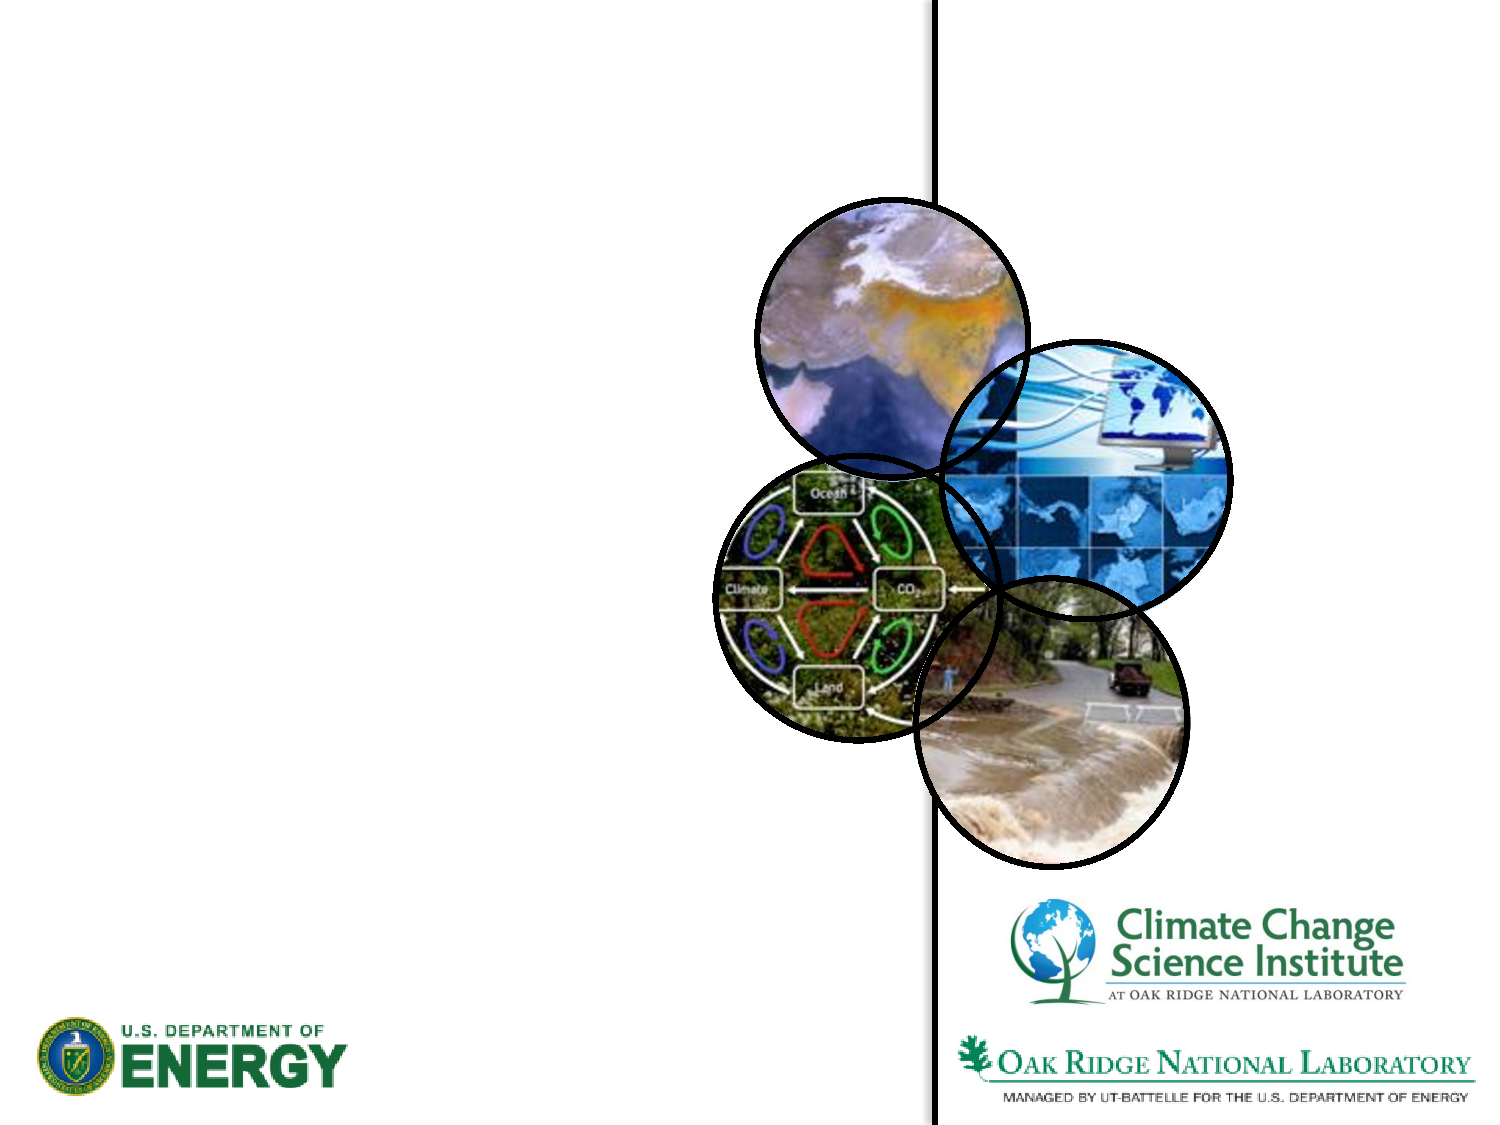
\includegraphics[width=\paperwidth]{backgrounds/CCSI_title_background.pdf}}
\begin{frame}
 %\vskip-0.250in
 \vskip0.05in
 \parbox{0.5\textwidth}{\Large\raggedright\color{CCSIGreen}\bf
  % Put the title here:
  \inserttitle
 }
 \vskip0.10in
 \parbox{0.45\textwidth}{\scriptsize\raggedright\bf
  % Put the author list or subtitle here:
  \insertauthor
 }
 \vskip0.05in
 \parbox{0.45\textwidth}{\scriptsize\raggedright
  % Put the institution list here:
  \insertinstitute
 }
 %\vskip0.5in
 %\parbox{0.5\textwidth}{\small\raggedright\color{CCSIGreen}\bf
 % \insertinstitute
 %}
 \vskip0.10in
 \parbox{0.6\textwidth}{\scriptsize\raggedright\bf
  {\color{DarkBlue}
  Fourth Workshop on Understanding Climate Change from Data, Boulder, Colorado, USA
  } \\
 }
 \vskip0.10in
 \parbox{0.5\textwidth}{\footnotesize\raggedright\bf
  \insertdate
 }
 %\vbox{\vspace{0.05in}\hspace{1.50in}
\includegraphics[width=0.25\textwidth]{logos/ucirvine_07_sol_seal_lt_289.jpg}}
 \vbox{
  %\vspace{-0.20in}\hspace{2.10in}
\includegraphics[width=0.12\textwidth]{logos/USFS_Logo.png}}
  \vspace{-0.20in}\hspace{1.00in}
\includegraphics[height=0.15\textheight]{logos/uci_peter.png}\hspace{0.15in}
\includegraphics[height=0.15\textheight]{logos/USFS_Logo.png}}
 %\vbox{
 % \vspace{-0.50in}\hspace{2.10in}
\includegraphics[width=0.125\textwidth]{logos/ess_logo_white.pdf} \\
 % \hspace{1.60in}
\includegraphics[width=0.25\textwidth]{logos/ucirvine_07_sol_seal_lt_289.jpg}}
\end{frame}
}

%%%%%%%%%%%%%%%%%%%%%%%%%%%%%%%%%%%%%%%%%%%%%%%%%%%%%%%%%%%%%%%%%%%%%%%%%%%%%%%
% Data Mining for Climate Change Model Intercomparison (view on browser)
%%%%%%%%%%%%%%%%%%%%%%%%%%%%%%%%%%%%%%%%%%%%%%%%%%%%%%%%%%%%%%%%%%%%%%%%%%%%%%%
%\section[Model Intercomparison]{Data Mining for Climate Change Model Intercomparison}
%%%%%%%%%%%%%%%%%%%%%%%%%%%%%%%%%%%%%%%%%%%%%%%%%%%%%%%%%%%%%%%%%%%%%%%%%%%%%%%
%\begin{frame}
% %\frametitle{}
% \begin{center}
%  \textbf{\Huge\color{CCSIGreen}Data Mining for Climate Change Model Intercomparison} \\
%  \vskip1in
%  \cite{Hoffman_EI_20050803}
% \end{center}
%\end{frame}
%%%%%%%%%%%%%%%%%%%%%%%%%%%%%%%%%%%%%%%%%%%%%%%%%%%%%%%%%%%%%%%%%%%%%%%%%%%%%%%

%%%%%%%%%%%%%%%%%%%%%%%%%%%%%%%%%%%%%%%%%%%%%%%%%%%%%%%%%%%%%%%%%%%%%%%%%%%%%%%
% Sampling Domain Representativeness
%%%%%%%%%%%%%%%%%%%%%%%%%%%%%%%%%%%%%%%%%%%%%%%%%%%%%%%%%%%%%%%%%%%%%%%%%%%%%%%
\section[Representativeness]{Sampling Domain Representativeness}
\subsection[NGEE Arctic]{Next-Generation Ecosystem Experiments (NGEE Arctic)}
%%%%%%%%%%%%%%%%%%%%%%%%%%%%%%%%%%%%%%%%%%%%%%%%%%%%%%%%%%%%%%%%%%%%%%%%%%%%%%%
\begin{frame}
 \begin{center}
  \vskip-0.15in
  \begin{block}{}\centering
   \textbf{\color{CCSIGreen}Next-Generation Ecosystem Experiments (NGEE Arctic) \\
   \url{http://ngee.ornl.gov/}}
  \end{block}
  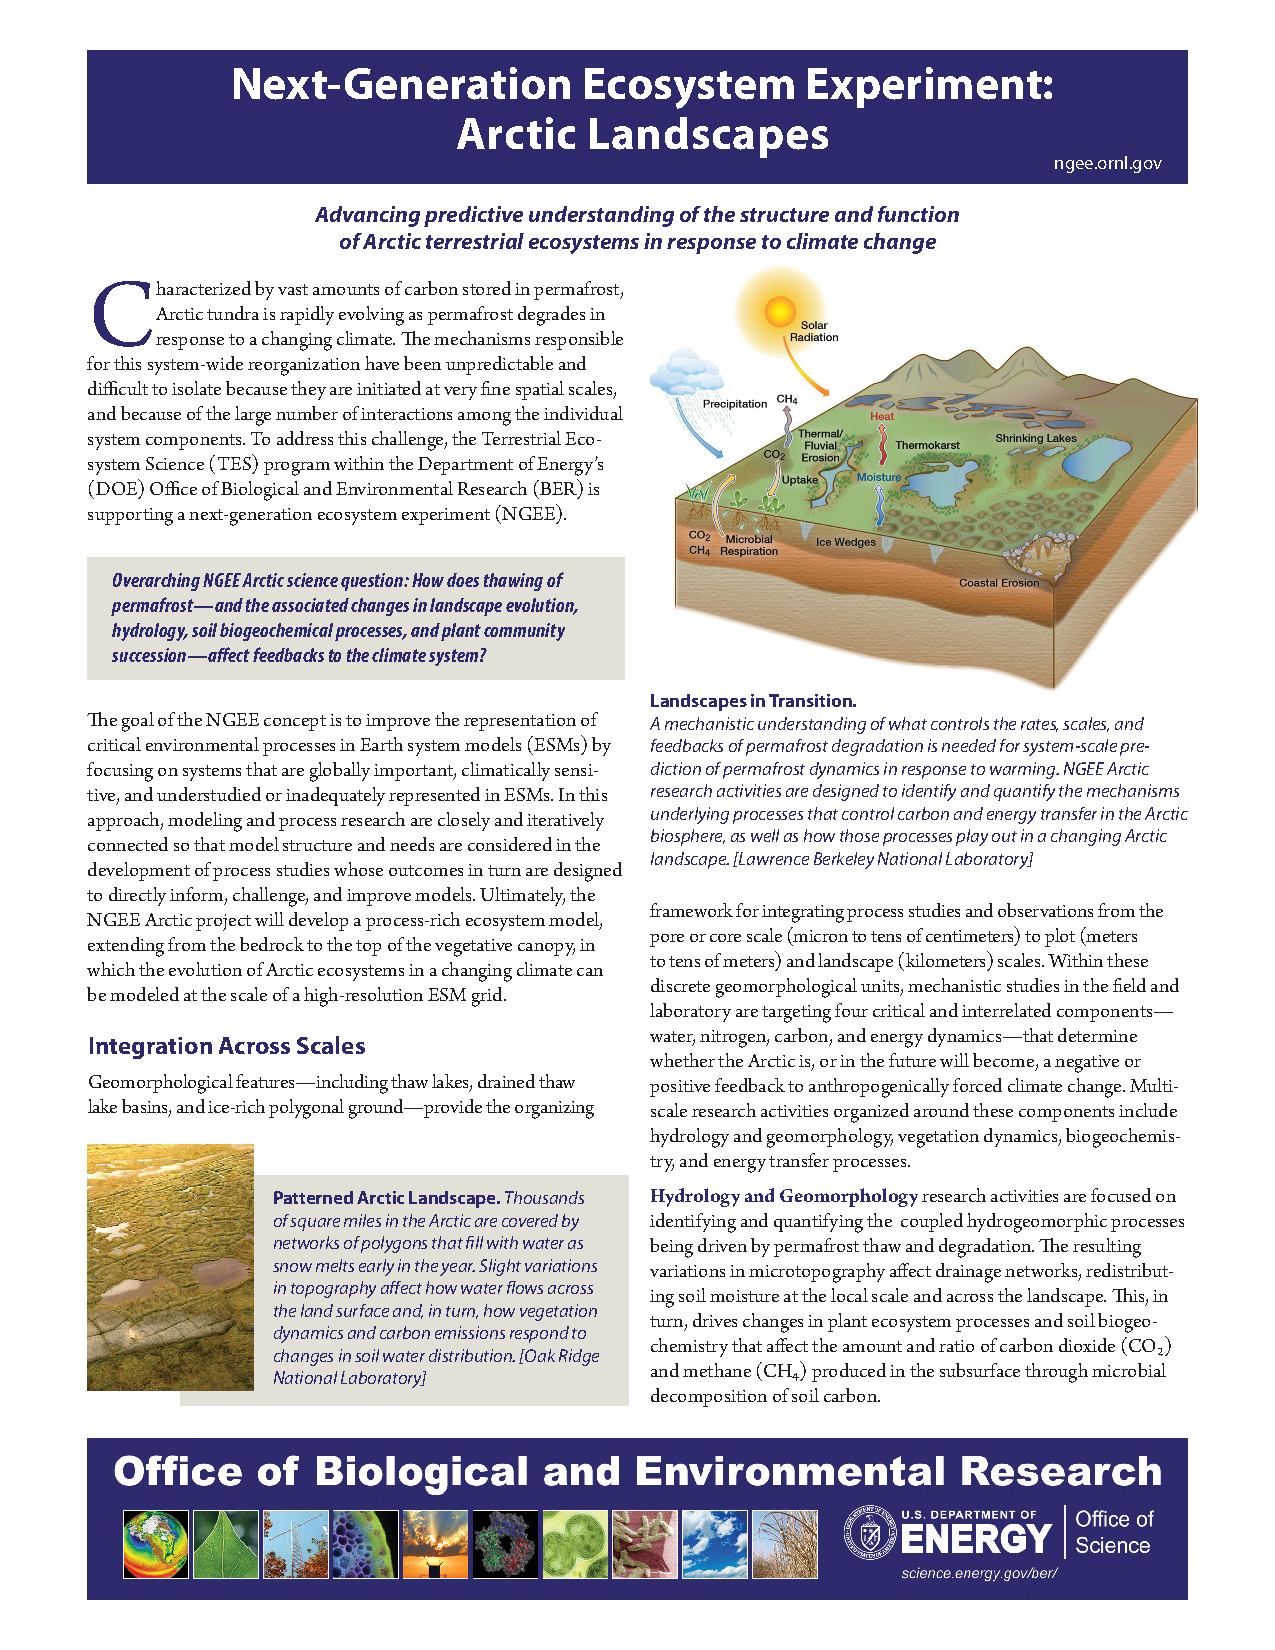
\includegraphics[width=0.74\textwidth,page=1,trim=4.25in 6.38in 0.5in 1.75in,clip=TRUE]{ngee_figures/TES-ArcticEco_07-25-2012d.pdf} \\
  %\vskip-0.25in
  \tiny\textit{The Next-Generation Ecosystem Experiments (NGEE Arctic) project is
supported by the Office of Biological and Environmental Research in the
DOE Office of Science.
}
 \end{center}
 \vskip-0.25in
 \begin{block}{}
  {
\includegraphics[height=0.05\paperheight]{logos/DOE_logo.png}\hfill
\includegraphics[height=0.07\paperheight]{logos/ORNL_logo.png}\hfill
\includegraphics[height=0.07\paperheight]{logos/LANL_logo.png}\hfill
\includegraphics[height=0.07\paperheight]{logos/LBNL_logo.png}\hfill
\includegraphics[height=0.07\paperheight]{logos/BNL_logo.png}\hfill
\includegraphics[height=0.07\paperheight]{logos/UAF_logo.png}}
 \end{block}
\end{frame}
%%%%%%%%%%%%%%%%%%%%%%%%%%%%%%%%%%%%%%%%%%%%%%%%%%%%%%%%%%%%%%%%%%%%%%%%%%%%%%%
\begin{frame}
 \frametitle{Integrating Across Scales}
 \begin{itemize}\small
  \item NGEE Arctic process studies and observations are strongly linked to model development and application for improving process representation, initialization, calibration, and evaluation.
  \item A hierarchy of models will be deployed at fine, intermediate, and climate scales to connect observations to models and models to each other in a quantitative up-scaling and down-scaling framework.
\end{itemize}
\begin{center}
  \includegraphics[width=\textwidth,page=2,trim=0.58in 7.75in 0.58in 0.325in,clip=TRUE]{ngee_figures/TES-ArcticEco_07-25-2012d.pdf} \\
 \end{center}
\end{frame}
%%%%%%%%%%%%%%%%%%%%%%%%%%%%%%%%%%%%%%%%%%%%%%%%%%%%%%%%%%%%%%%%%%%%%%%%%%%%%%%%
%
%
%%%%%%%%%%%%%%%%%%%%%%%%%%%%%%%%%%%%%%%%%%%%%%%%%%%%%%%%%%%%%%%%%%%%%%%%%%%%%%%
\subsection[Representativeness]{Representativeness-Based Network Design}
%\section{Introduction}
%%%%%%%%%%%%%%%%%%%%%%%%%%%%%%%%%%%%%%%%%%%%%%%%%%%%%%%%%%%%%%%%%%%%%%%%%%%%%%%
% NGEE-Arctic Site-representativeness introduction slide
%%%%%%%%%%%%%%%%%%%%%%%%%%%%%%%%%%%%%%%%%%%%%%%%%%%%%%%%%%%%%%%%%%%%%%%%%%%%%%%
%
%%
%% HOPEFULLY, slides motivating the need for the NGEE project itself will have
%% been presented for this last set of slides for the last 15 minutes of
%% tag-team presentations.
%%
%%\begin{frame}{Representativeness and Scaling}
%% \begin{itemize}
%%  \item Need for studies of the complex and interacting processes of the
%%atmosphere, sea ice, ocean, and terrestrial systems in Arctic to improve
%%the interpretation of past climate and projections of future climate.
%%  \item Committee on Designing an Arctic Observing Network  recommended an
%%Arctic Observing Network to satisfy current and future scientific by
%%monitoring key physical, biogeochemical, and human dimensions
%%variables.
%%  \item Conducting systematic and continuous field observations and long
%%term monitoring are challenging, particularly in the Arctic.
%% \end{itemize}
%%\end{frame}
%%
%
\begin{frame}
 %\frametitle{Representativeness and Scaling}
 \frametitle{Quantitative Sampling Network Design}
 \begin{itemize}
  \item Resource and logistical constraints limit the frequency and extent
  of observations, necessitating the development of a systematic sampling
  strategy that objectively represents environmental variability at the
  desired spatial scale.
  \item Required is a methodology that provides a quantitative framework
  for informing site selection and determining the representativeness
  of measurements.
  \item Multivariate spatiotemporal clustering (MSTC) was applied at
  the landscape scale (4~km$^2$) for the State of Alaska to demonstrate
  its utility for representativeness and scaling.
  \item An extension of the method applied by Hargrove and Hoffman for
  design of National Science Foundation's (NSF's) National Ecological
  Observatory Network (NEON) domains \citep{Schimel_FrontEcolEnviron_20070301,Keller_FrontEcolEnviron_20080601}.
 \end{itemize}

\end{frame}


%%%%%%%%%%%%%%%%%%%%%%%%%%%%%%%%%%%%%%%%%%%%%%%%%%%%%%%%%%%%%%%%%%%%%%%%%%%%%%%
\begin{frame}{Multivariate Spatiotemporal Clustering (MSTC)}
 \vskip-0.15in
 \begin{figure}
  \begin{center}
   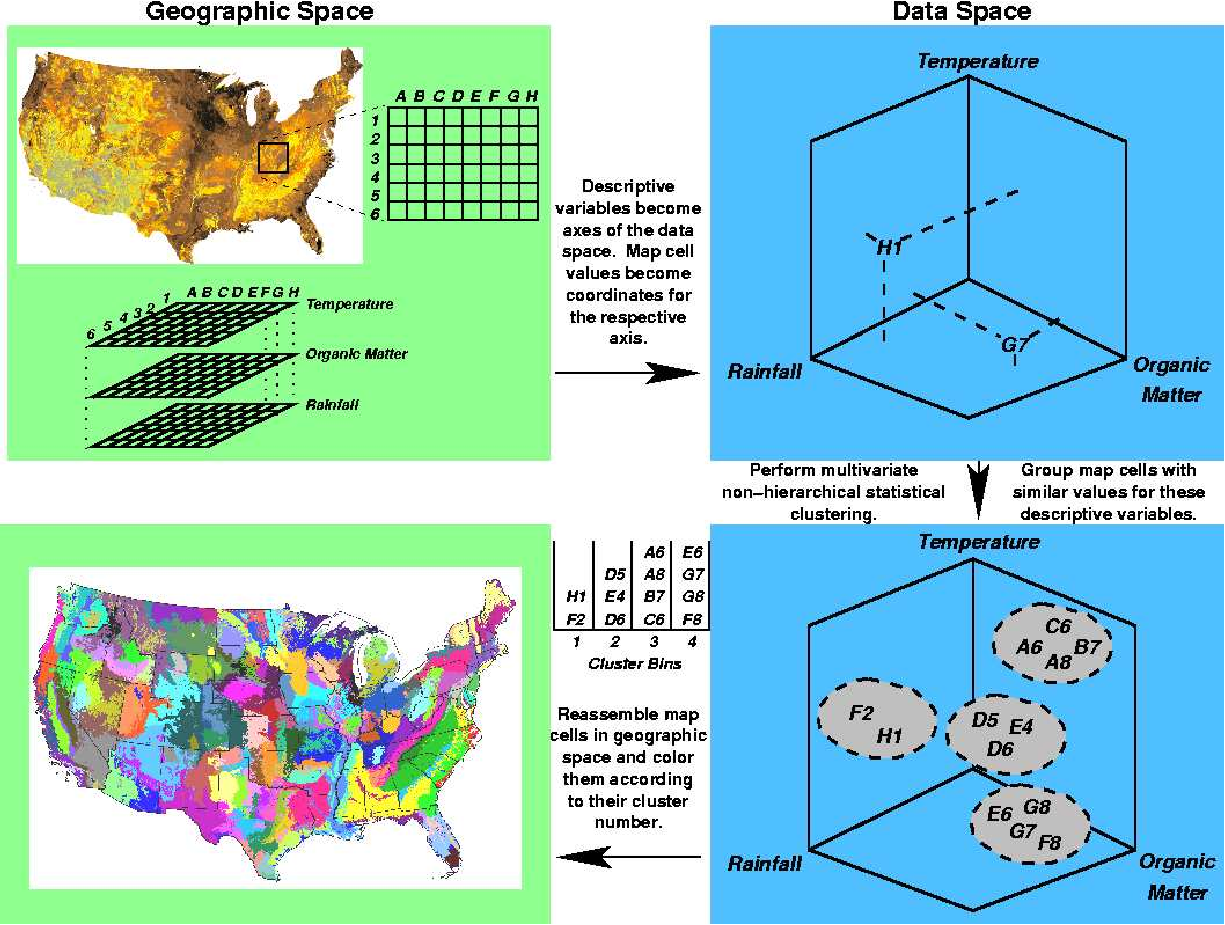
\includegraphics[width=0.91\textwidth]{ngee_figures/clusterfinal3}
  \end{center}
  %\caption{Cluster analysis.}
%  \label{fig:clusterfinal3}
 \end{figure}
\end{frame}
%%%%%%%%%%%%%%%%%%%%%%%%%%%%%%%%%%%%%%%%%%%%%%%%%%%%%%%%%%%%%%%%%%%%%%%%%%%%%%%

\subsection{Data Layers}

%%%%%%%%%%%%%%%%%%%%%%%%%%%%%%%%%%%%%%%%%%%%%%%%%%%%%%%%%%%%%%%%%%%%%%%%%%%%%%%
\begin{frame}{Data Layers}\footnotesize
 \begin{table}
 \vskip-0.15in
 \scriptsize%\tiny
  \caption{37 variables averaged for 2000--2009 and 2090--2099}\label{tbl:characteristics}
  \centering
  \begin{tabular}{m{4.2cm}ccc}
   \toprule
   Description & Number/Name & Units & Source \\
   \midrule
   Monthly mean air temperature                   & 12                 & $^\circ$C   & GCM \\
   Monthly mean precipitation                     & 12                 & mm          & GCM \\
   \multirow{2}{*}{Day of freeze}                 & mean               & day of year & GCM \\
                                                  & standard deviation & days        & \\
   \multirow{2}{*}{Day of thaw}                   & mean               & day of year & GCM \\
                                                  & standard deviation & days        & \\
   \multirow{2}{*}{Length of growing season}      & mean               & days        & GCM \\
                                                  & standard deviation & days        & \\
   Maximum active layer thickness                 & 1                  & m           & GIPL \\
   Warming effect of snow                         & 1                  & $^\circ$C   & GIPL \\
   Mean annual ground temperature at bottom of active layer & 1                  & $^\circ$C   & GIPL \\
   Mean annual ground surface temperature         & 1                  & $^\circ$C   & GIPL \\
   Thermal offset                                 & 1                  & $^\circ$C   & GIPL \\
   Limnicity                                      & 1                  & \%          & NHD \\
   Elevation                                      & 1                  & m           & SRTM \\
   \bottomrule
  \end{tabular}
\end{table}


\end{frame}
%%%%%%%%%%%%%%%%%%%%%%%%%%%%%%%%%%%%%%%%%%%%%%%%%%%%%%%%%%%%%%%%%%%%%%%%%%%%%%%

\subsection[Ecoregions]{Alaska Ecoregions}

%%%%%%%%%%%%%%%%%%%%%%%%%%%%%%%%%%%%%%%%%%%%%%%%%%%%%%%%%%%%%%%%%%%%%%%%%%%%%%%
\begin{frame}
 \frametitle{10 Alaska Ecoregions (2000--2009)}
 \begin{figure}
  \begin{center}
   \vskip-0.20in
   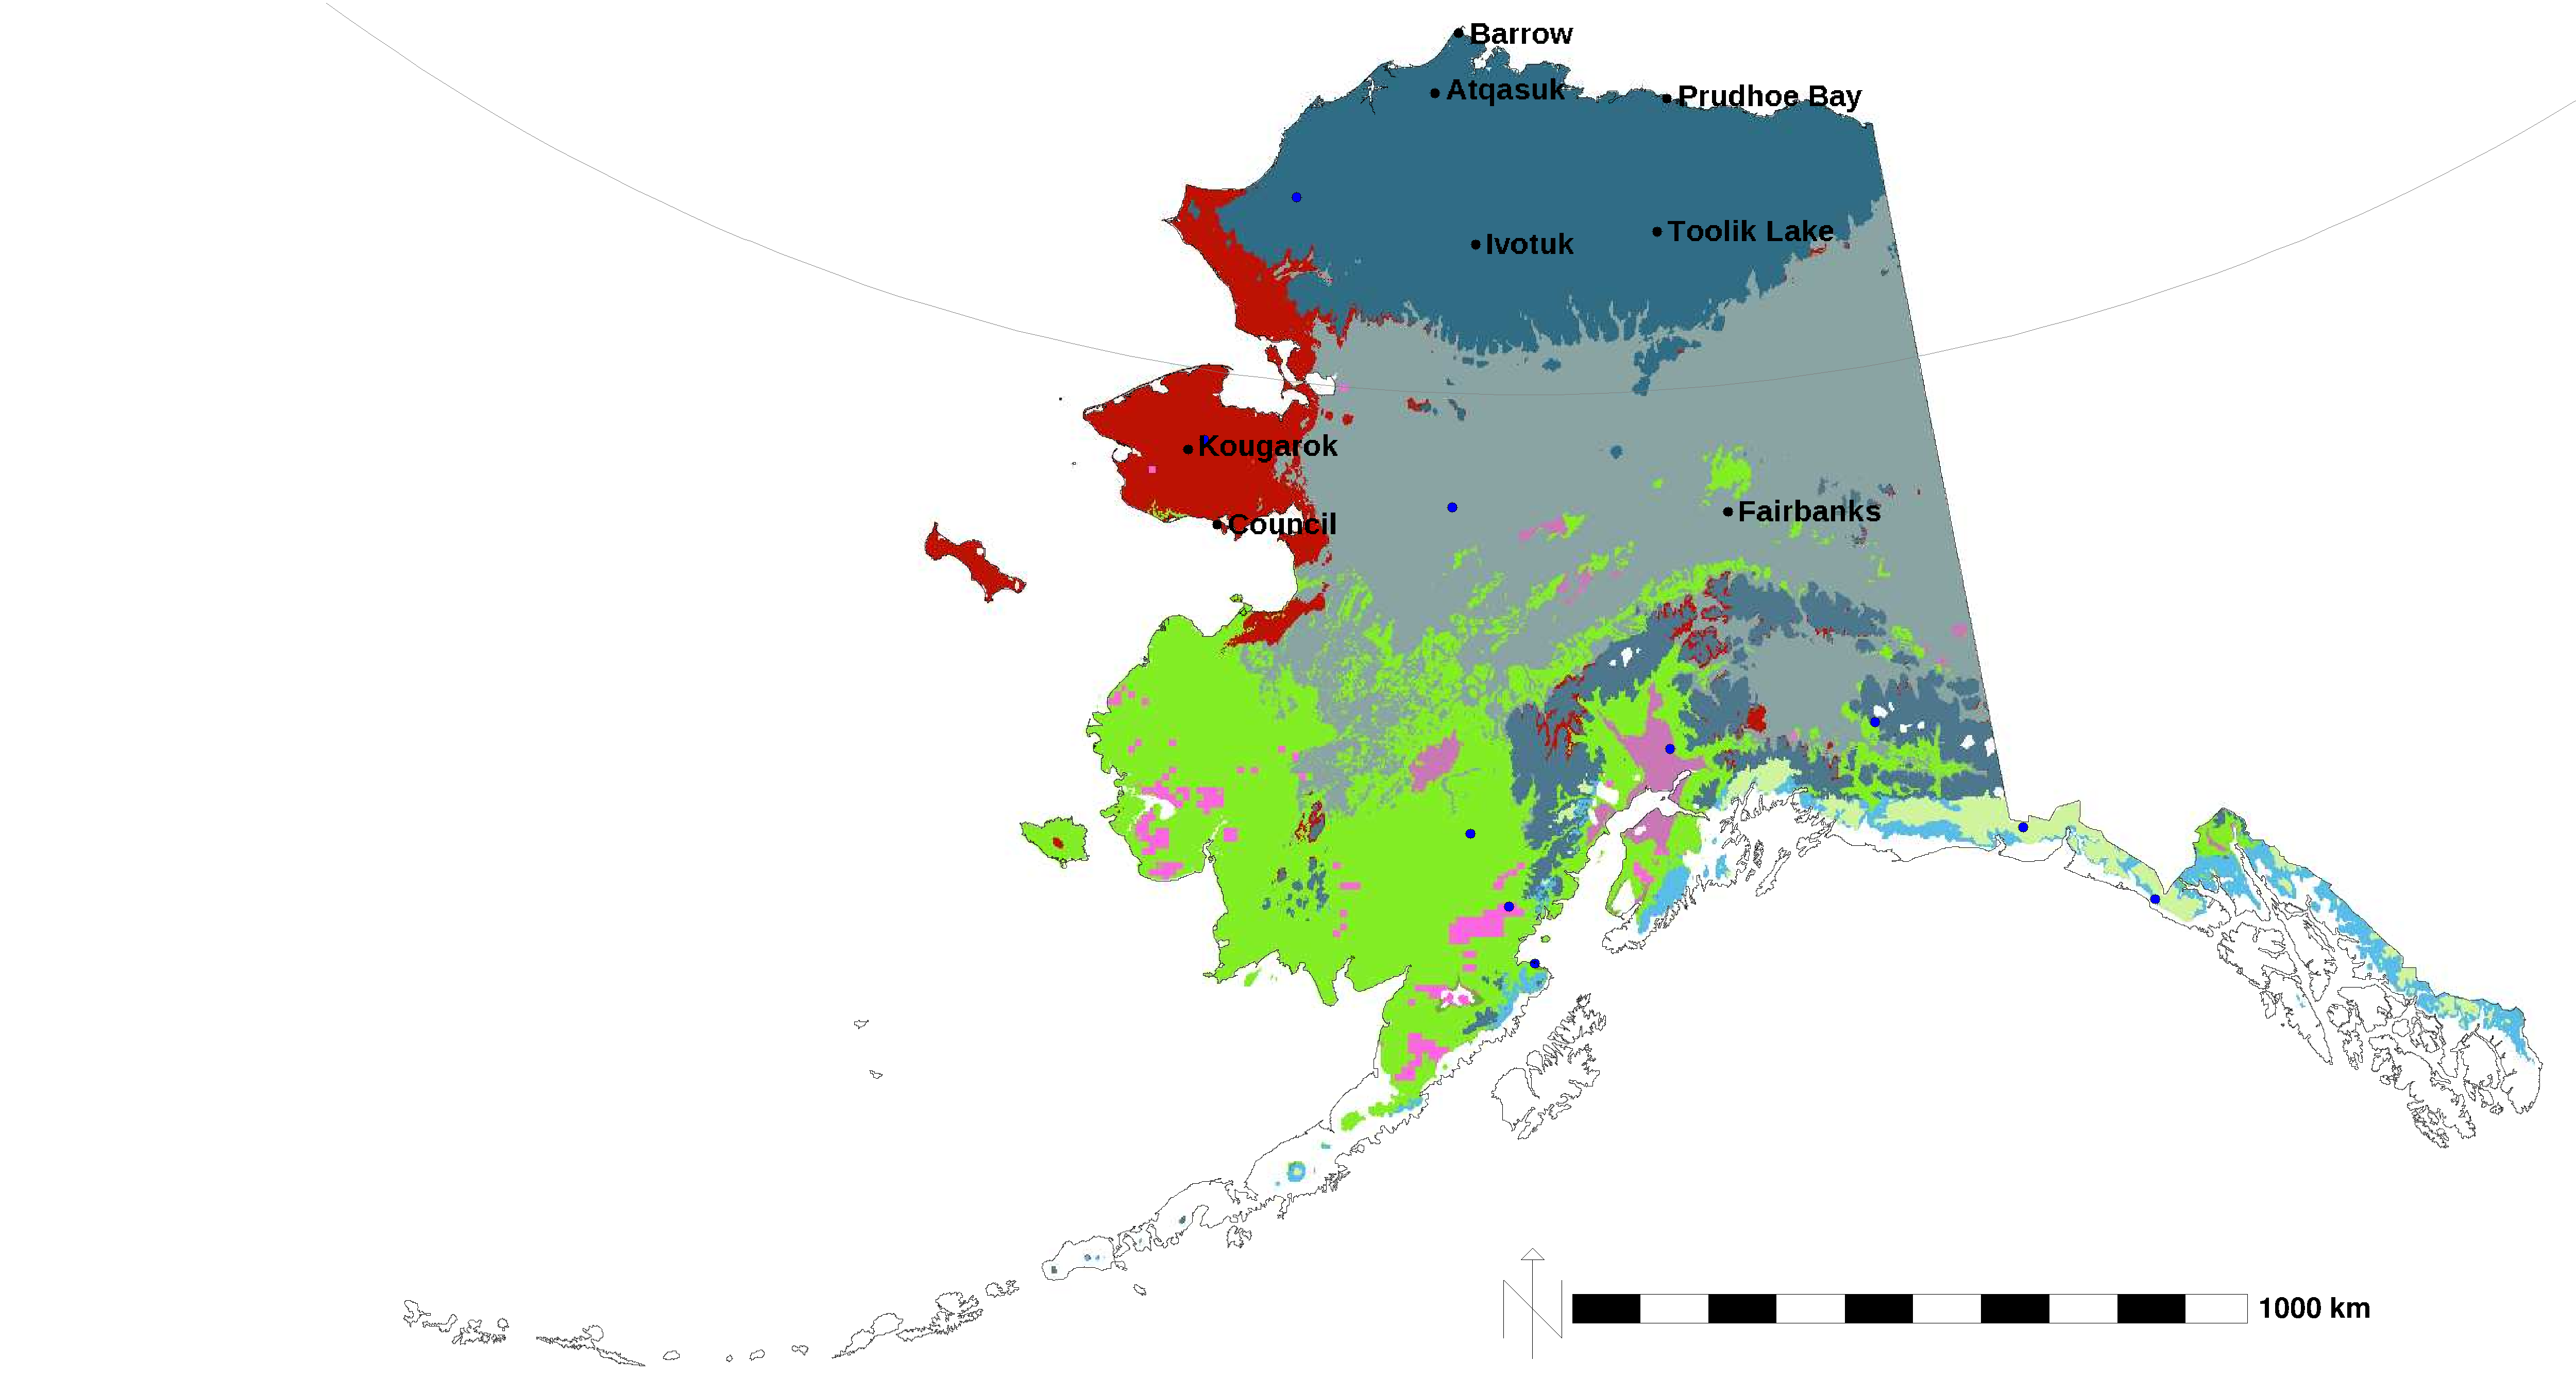
\includegraphics[width=\textwidth]{ngee_figures/alaska_dem_Feb2012_10_2000-2009_barscale}
  \end{center}
  %\caption{Cluster analysis.}
  \label{fig:alaska_2000_2009_10}
 \end{figure}
 \vskip-0.10in
 \vbox{\scriptsize\hfill\citep{Hoffman_LandscapeEcol_20131001}}
\smallskip
Each ecoregion is a different random color. Blue filled circles mark
locations most representative of mean conditions of each region.
\end{frame}
%%%%%%%%%%%%%%%%%%%%%%%%%%%%%%%%%%%%%%%%%%%%%%%%%%%%%%%%%%%%%%%%%%%%%%%%%%%%%%%

%%%%%%%%%%%%%%%%%%%%%%%%%%%%%%%%%%%%%%%%%%%%%%%%%%%%%%%%%%%%%%%%%%%%%%%%%%%%%%%
\begin{frame}
 \frametitle{10 Alaska Ecoregions (2090--2099)}
 \vskip-0.20in
 \begin{figure}
  \begin{center}
   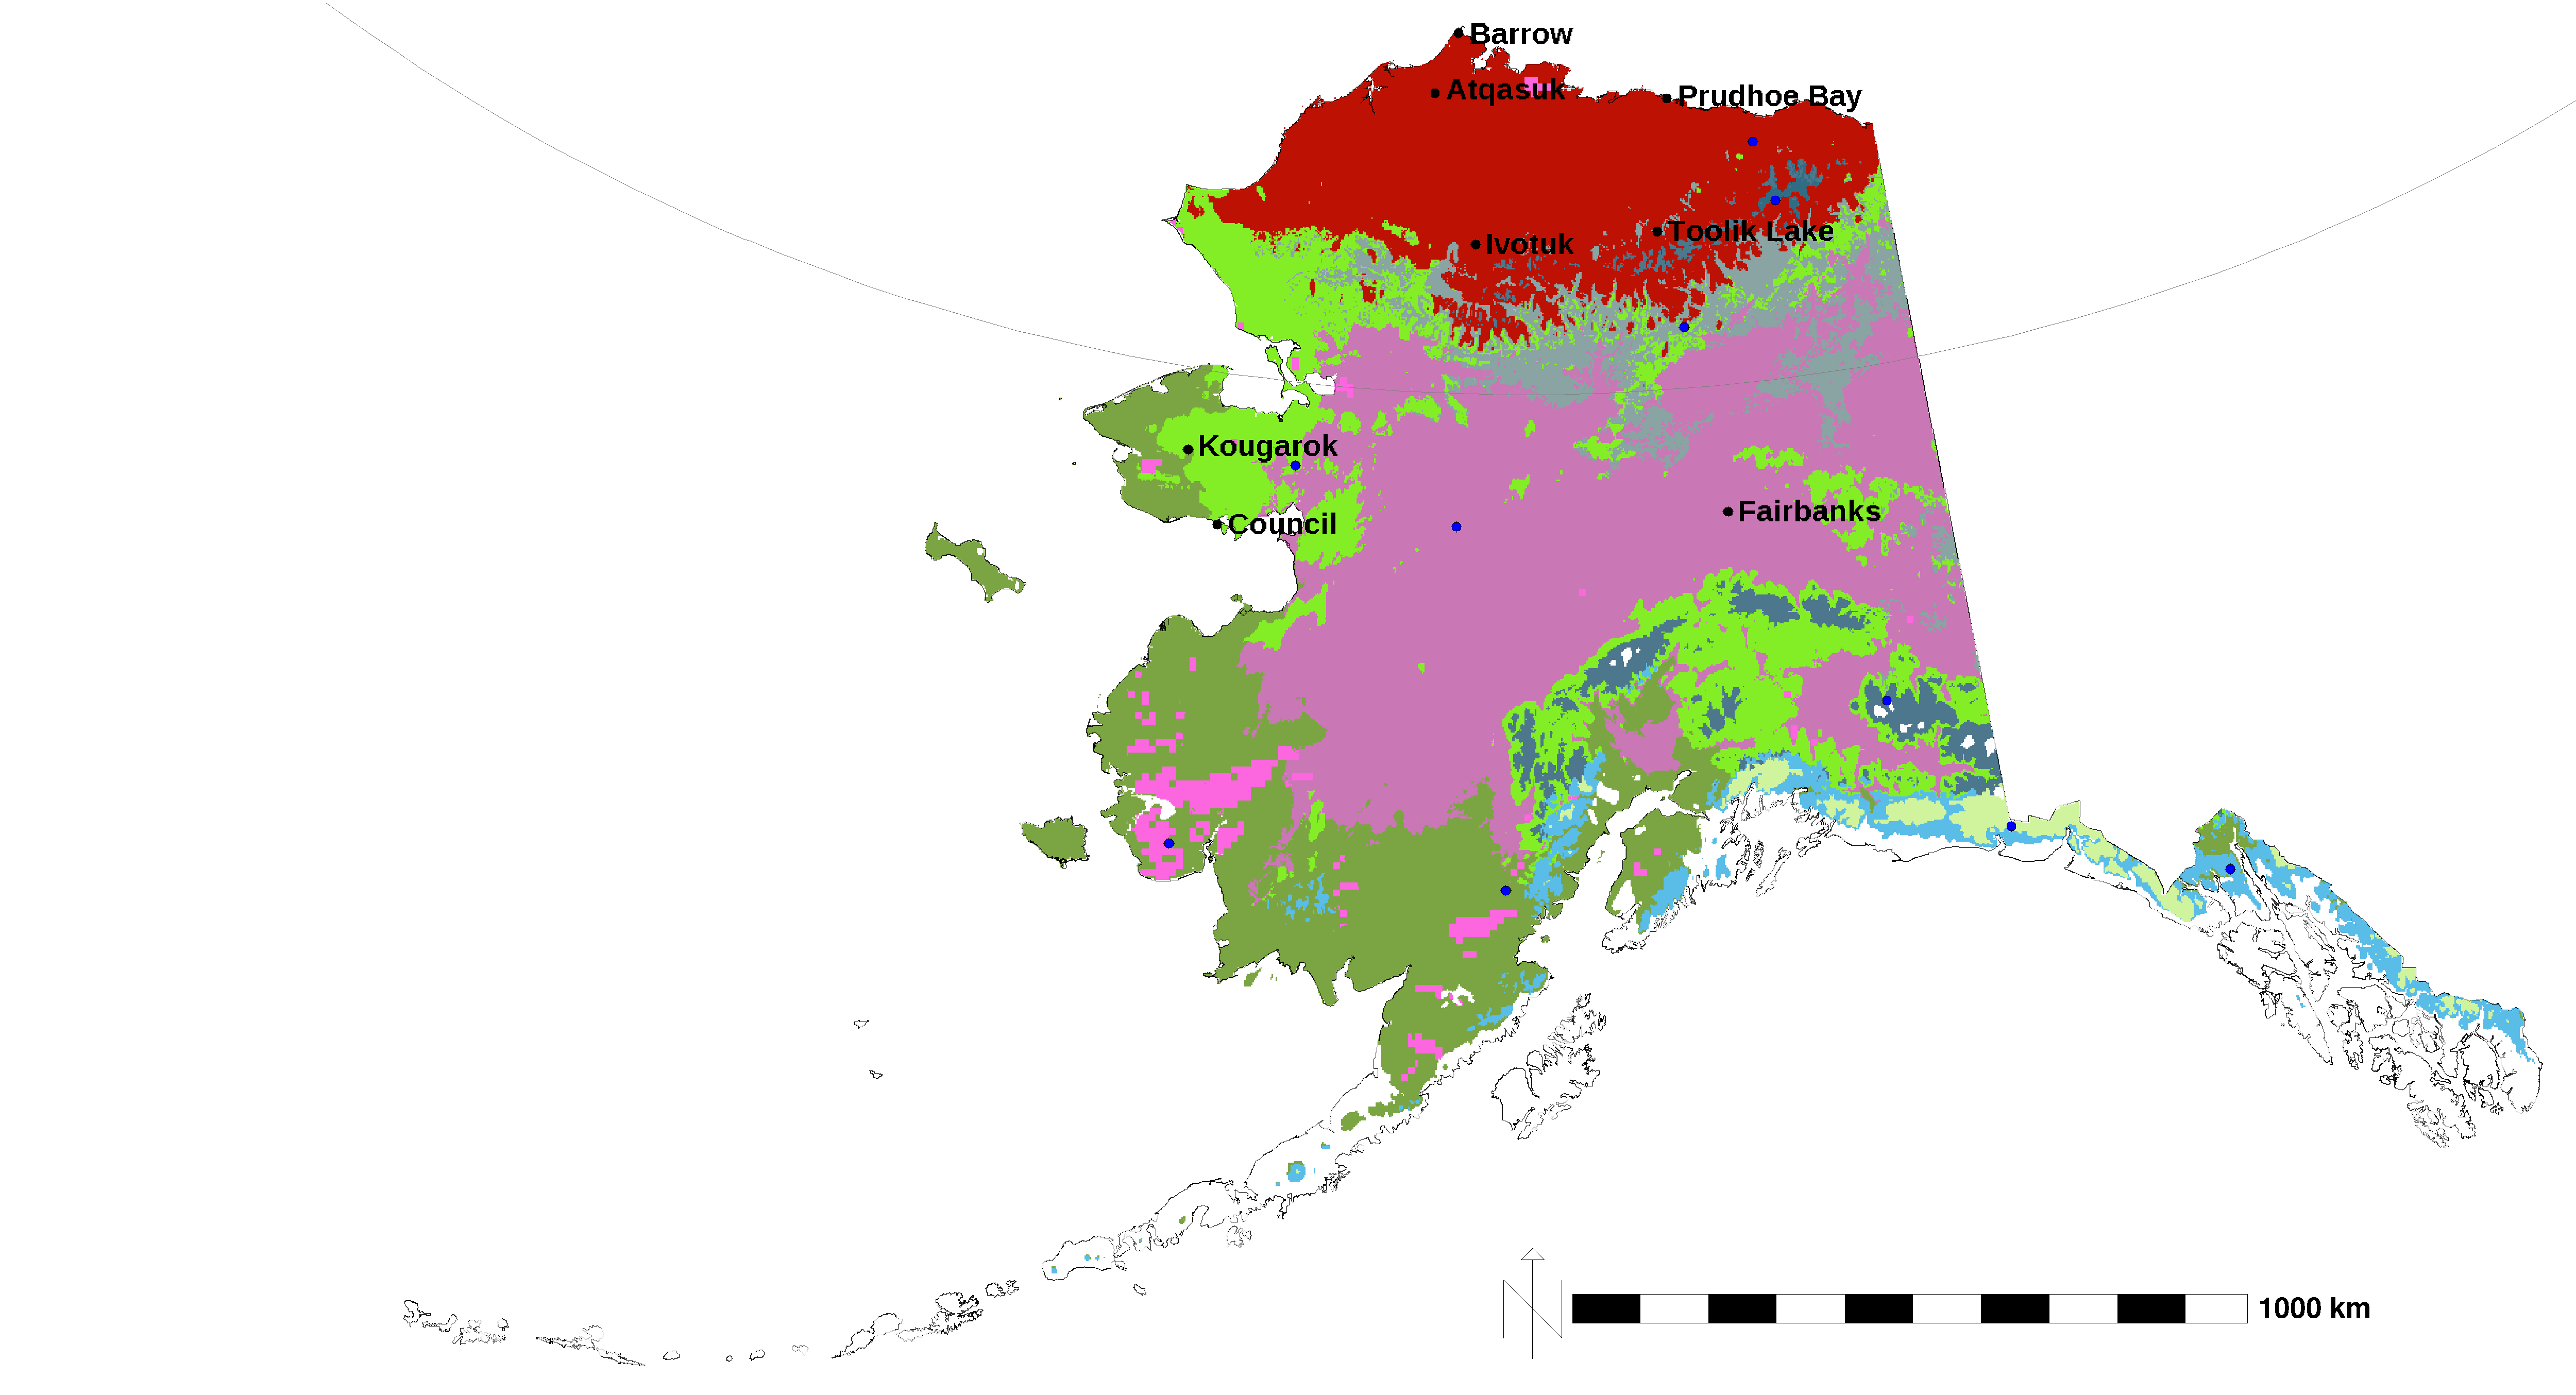
\includegraphics[width=\textwidth]{ngee_figures/alaska_dem_Feb2012_10_2090-2099_barscale}
  \end{center}
  %\caption{Cluster analysis.}
  \label{fig:alaska_2090_2099_10}
 \end{figure}
 \vskip-0.10in
 \vbox{\scriptsize\hfill\citep{Hoffman_LandscapeEcol_20131001}}
\smallskip
Each ecoregion is a different random color. Blue filled circles mark
locations most representative of mean conditions of each region.
\end{frame}
%%%%%%%%%%%%%%%%%%%%%%%%%%%%%%%%%%%%%%%%%%%%%%%%%%%%%%%%%%%%%%%%%%%%%%%%%%%%%%%

%%%%%%%%%%%%%%%%%%%%%%%%%%%%%%%%%%%%%%%%%%%%%%%%%%%%%%%%%%%%%%%%%%%%%%%%%%%%%%%
\begin{frame}
 \frametitle{10 Alaska Ecoregions, Present and Future}
 \vskip-0.15in
 \setlength{\tabcolsep}{0pt}
 \begin{figure}
   \begin{tabular}{cc}
   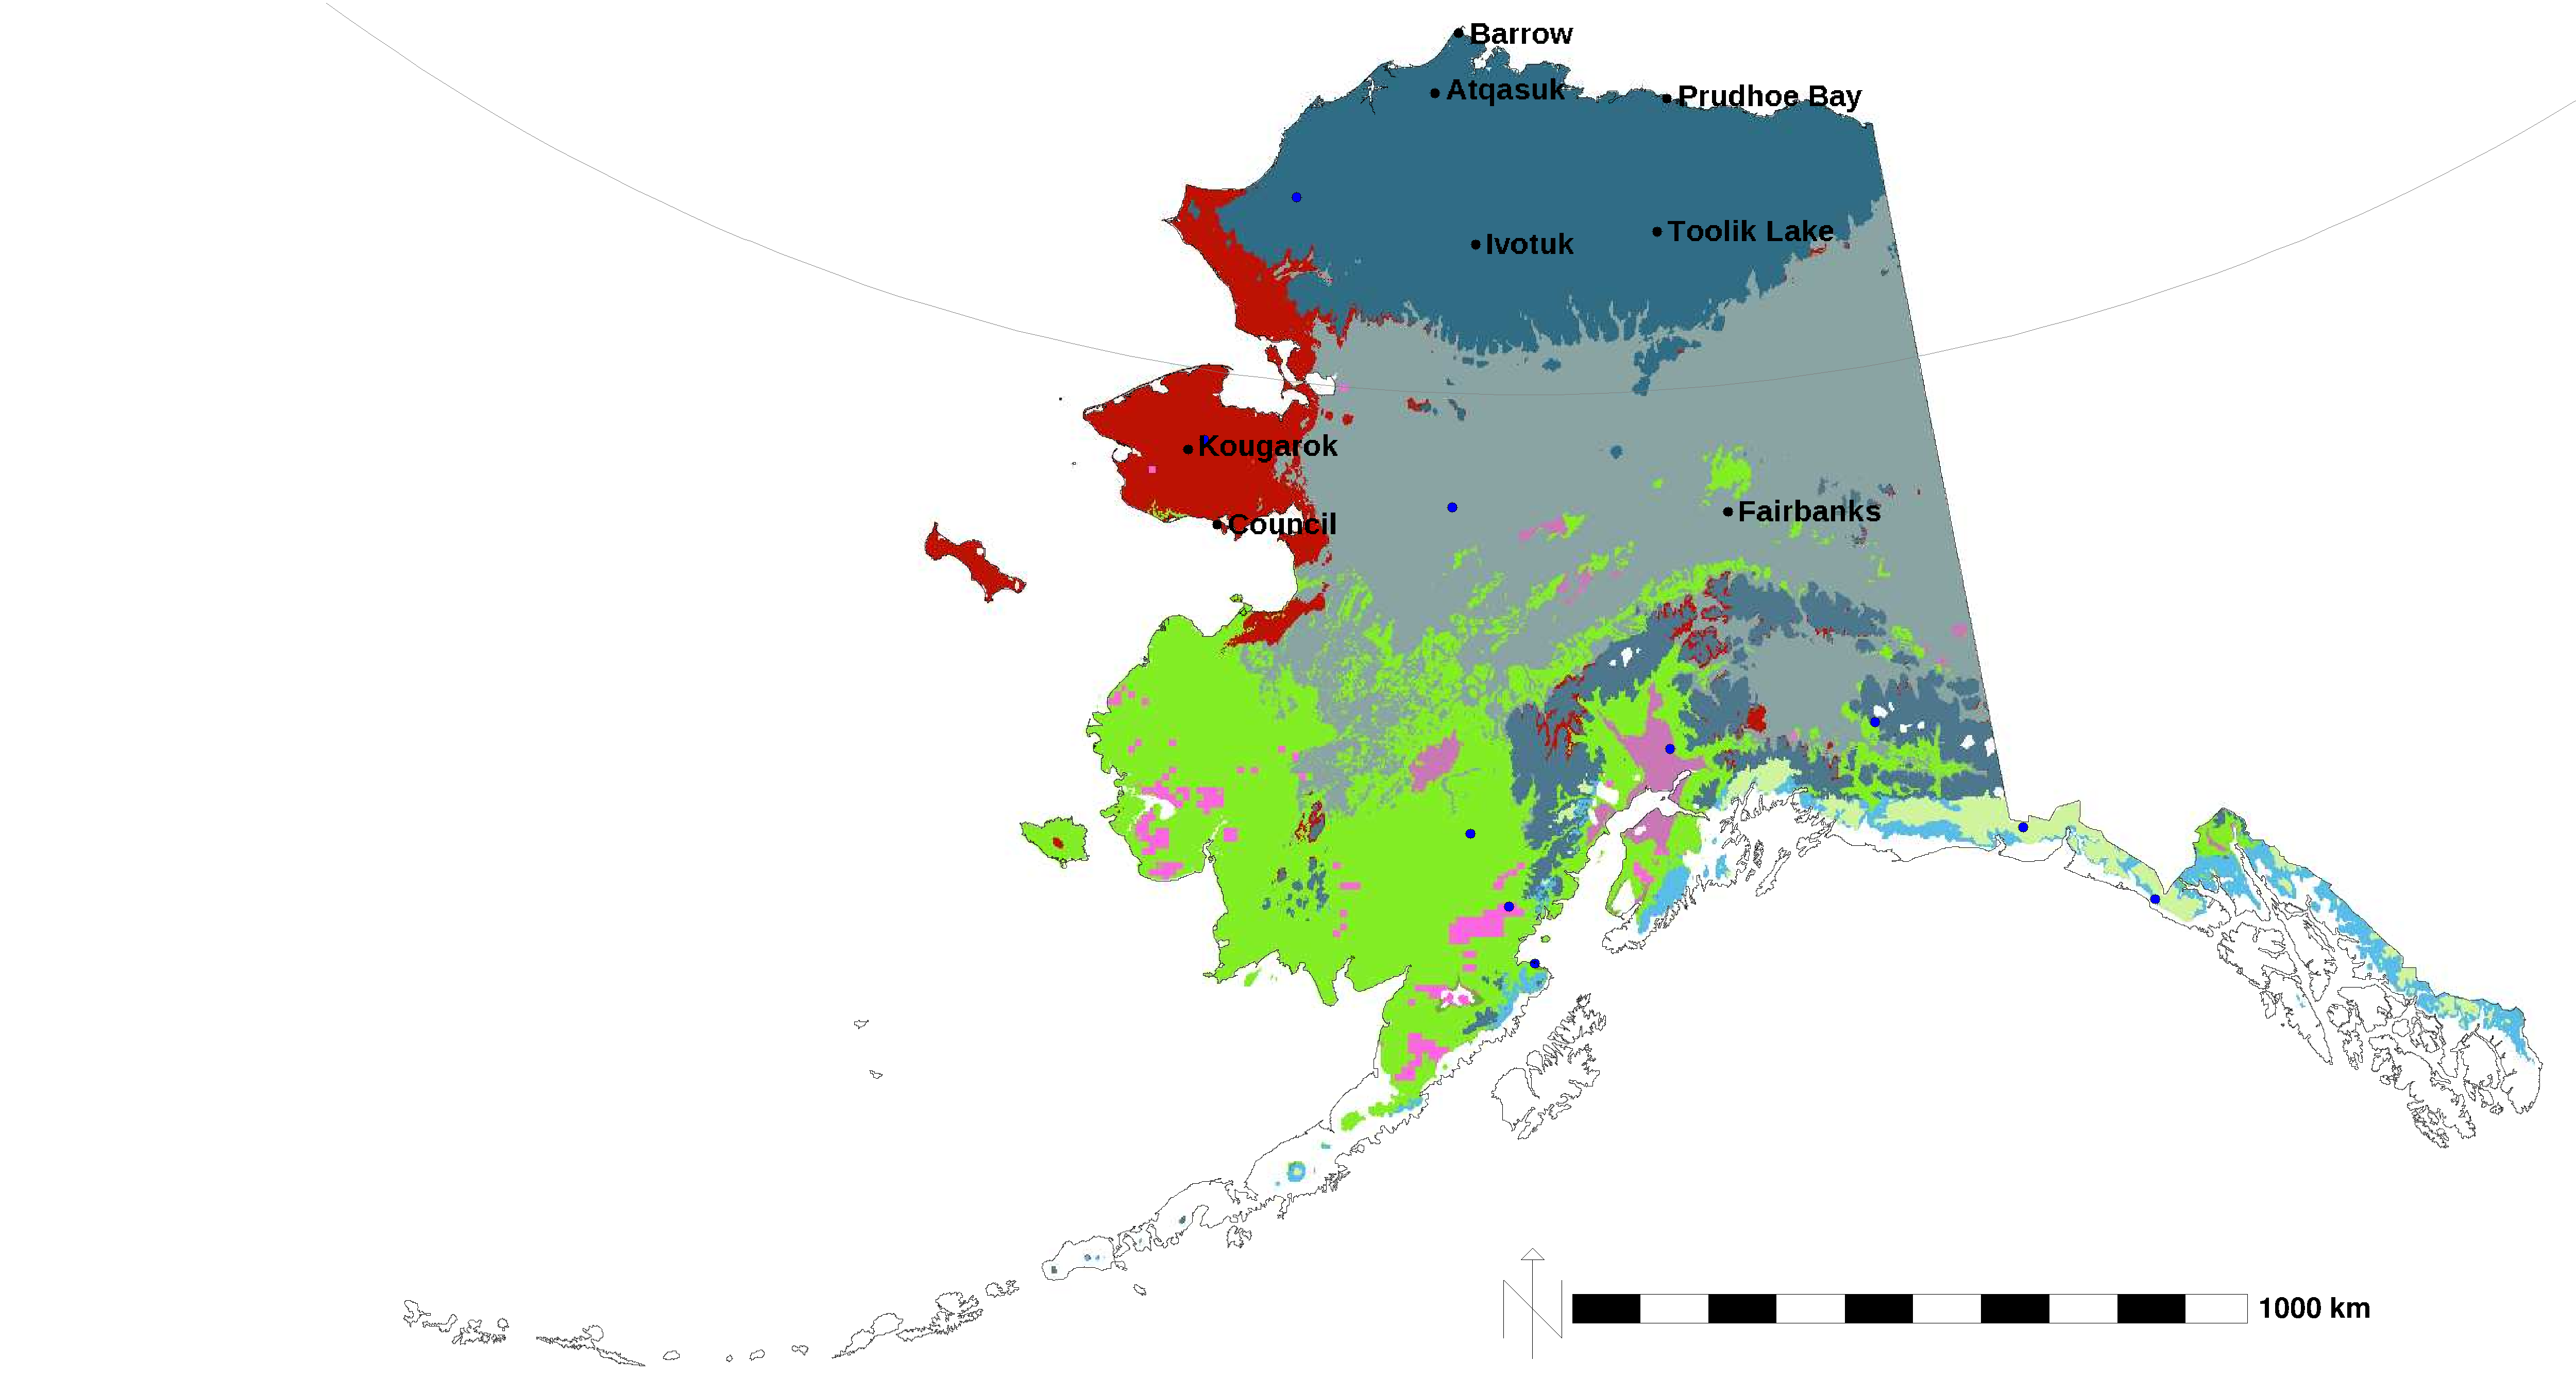
\includegraphics[width=0.50\textwidth]{ngee_figures/alaska_dem_Feb2012_10_2000-2009_barscale} &
   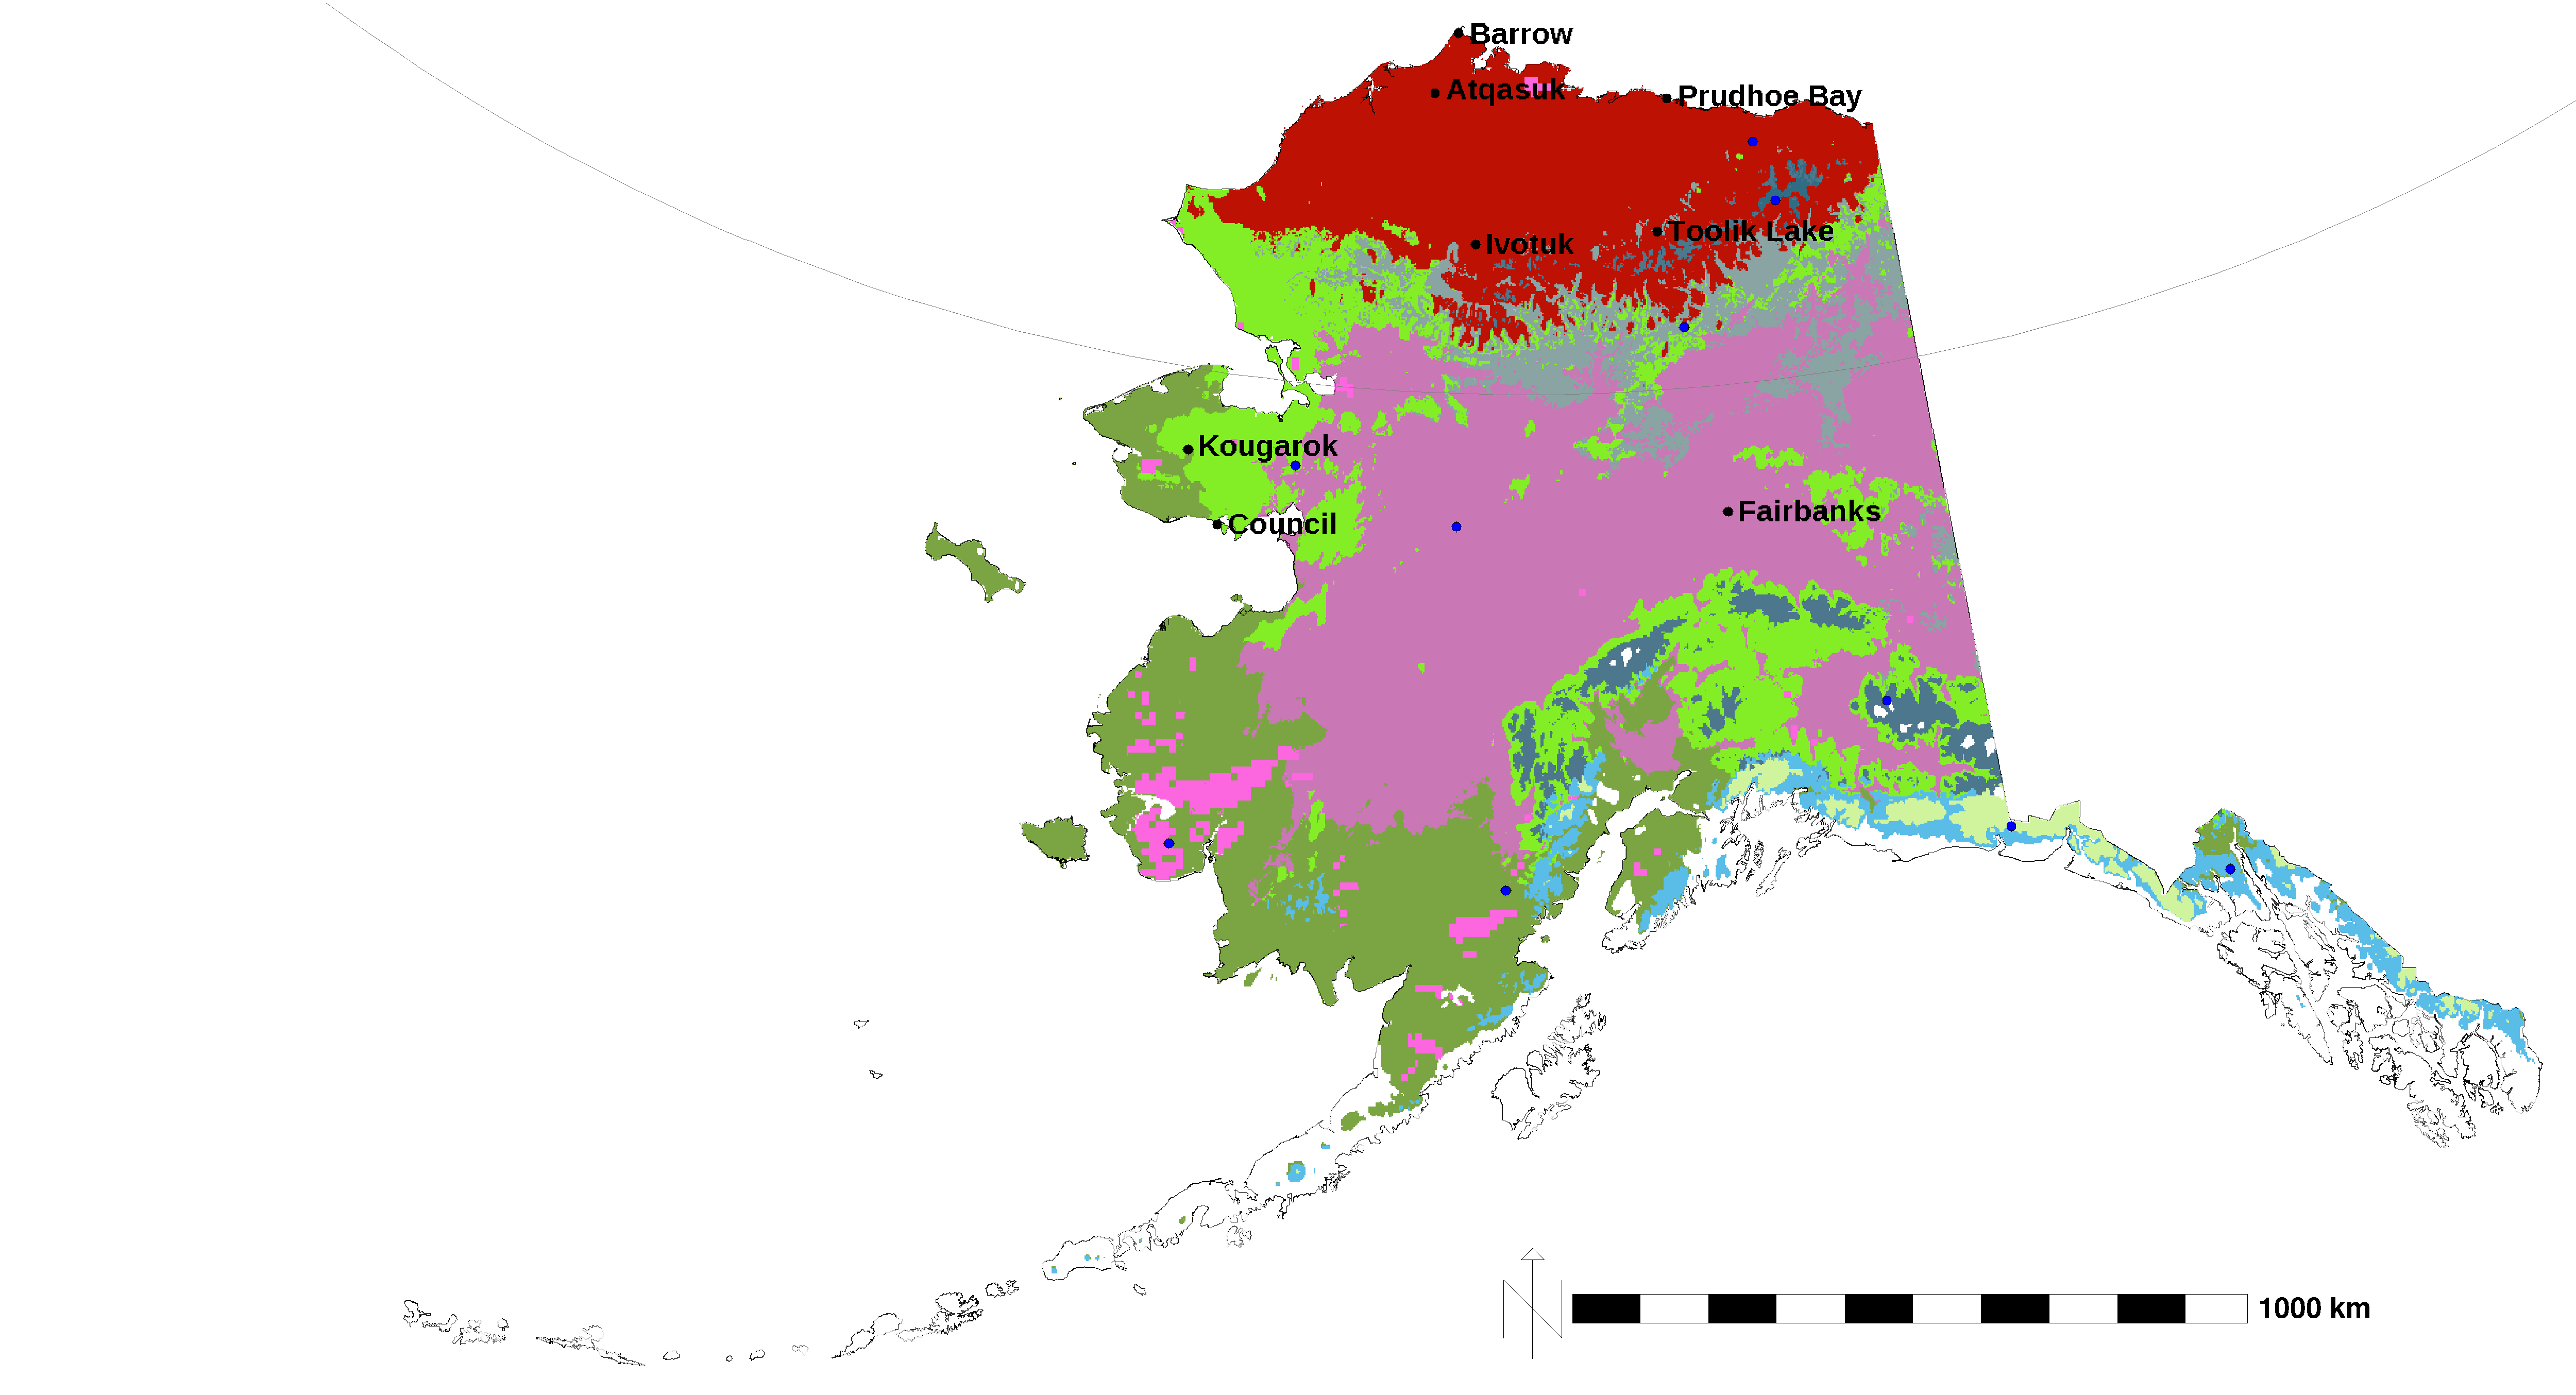
\includegraphics[width=0.50\textwidth]{ngee_figures/alaska_dem_Feb2012_10_2090-2099_barscale} \\
   2000--2009 & 2090--2099 \\
   \end{tabular}
  \vbox{\scriptsize\hfill\citep{Hoffman_LandscapeEcol_20131001}}
  %\caption{Cluster analysis.}
  \label{fig:alaska_both_10}
 \end{figure}
 \vskip-0.15in
\emph{Since the random colors are the same in both maps, a change in color
represents an environmental change between the present and the future.}\\

At this level of division, the conditions in the large boreal forest
become compressed onto the Brooks Range and the conditions on
the Seward Peninsula ``migrate'' to the North Slope.

\end{frame}
%%%%%%%%%%%%%%%%%%%%%%%%%%%%%%%%%%%%%%%%%%%%%%%%%%%%%%%%%%%%%%%%%%%%%%%%%%%%%%%

%%%%%%%%%%%%%%%%%%%%%%%%%%%%%%%%%%%%%%%%%%%%%%%%%%%%%%%%%%%%%%%%%%%%%%%%%%%%%%%
\begin{frame}
 \frametitle{20 Alaska Ecoregions, Present and Future}
 \vskip-0.15in
 \setlength{\tabcolsep}{0pt}
 \begin{figure}
   \begin{tabular}{cc}
   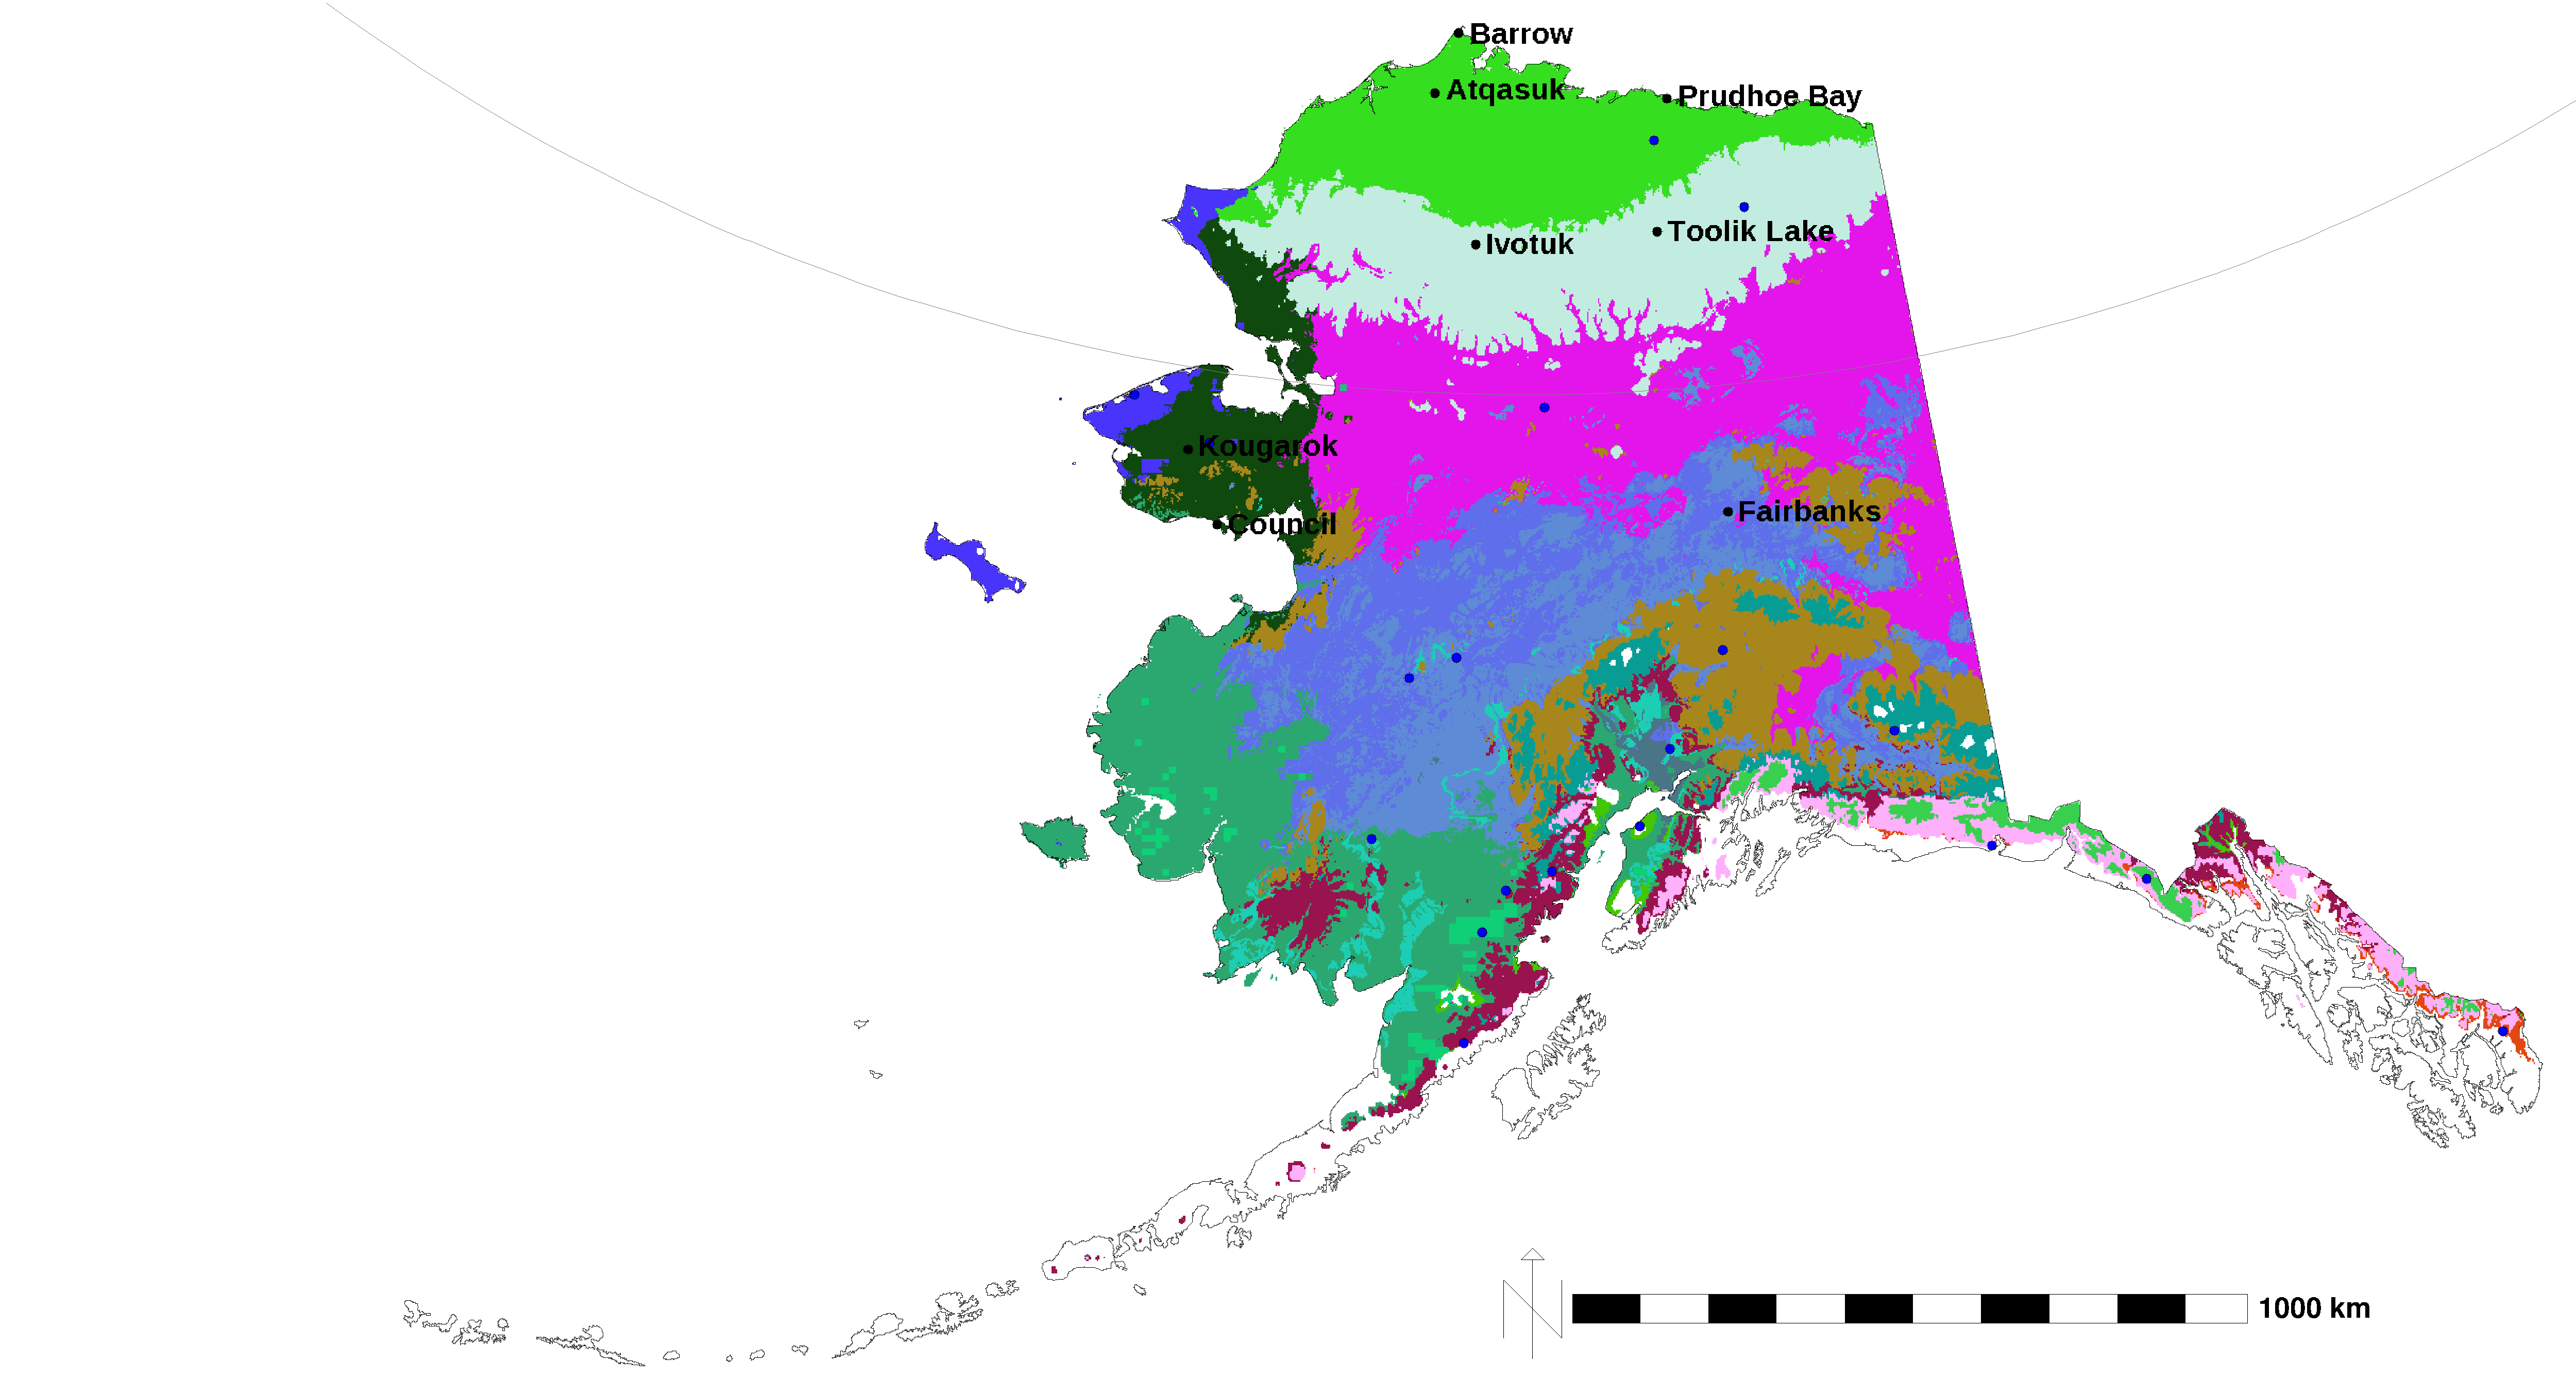
\includegraphics[width=0.50\textwidth]{ngee_figures/alaska_dem_Feb2012_20_2000-2009_barscale} &
   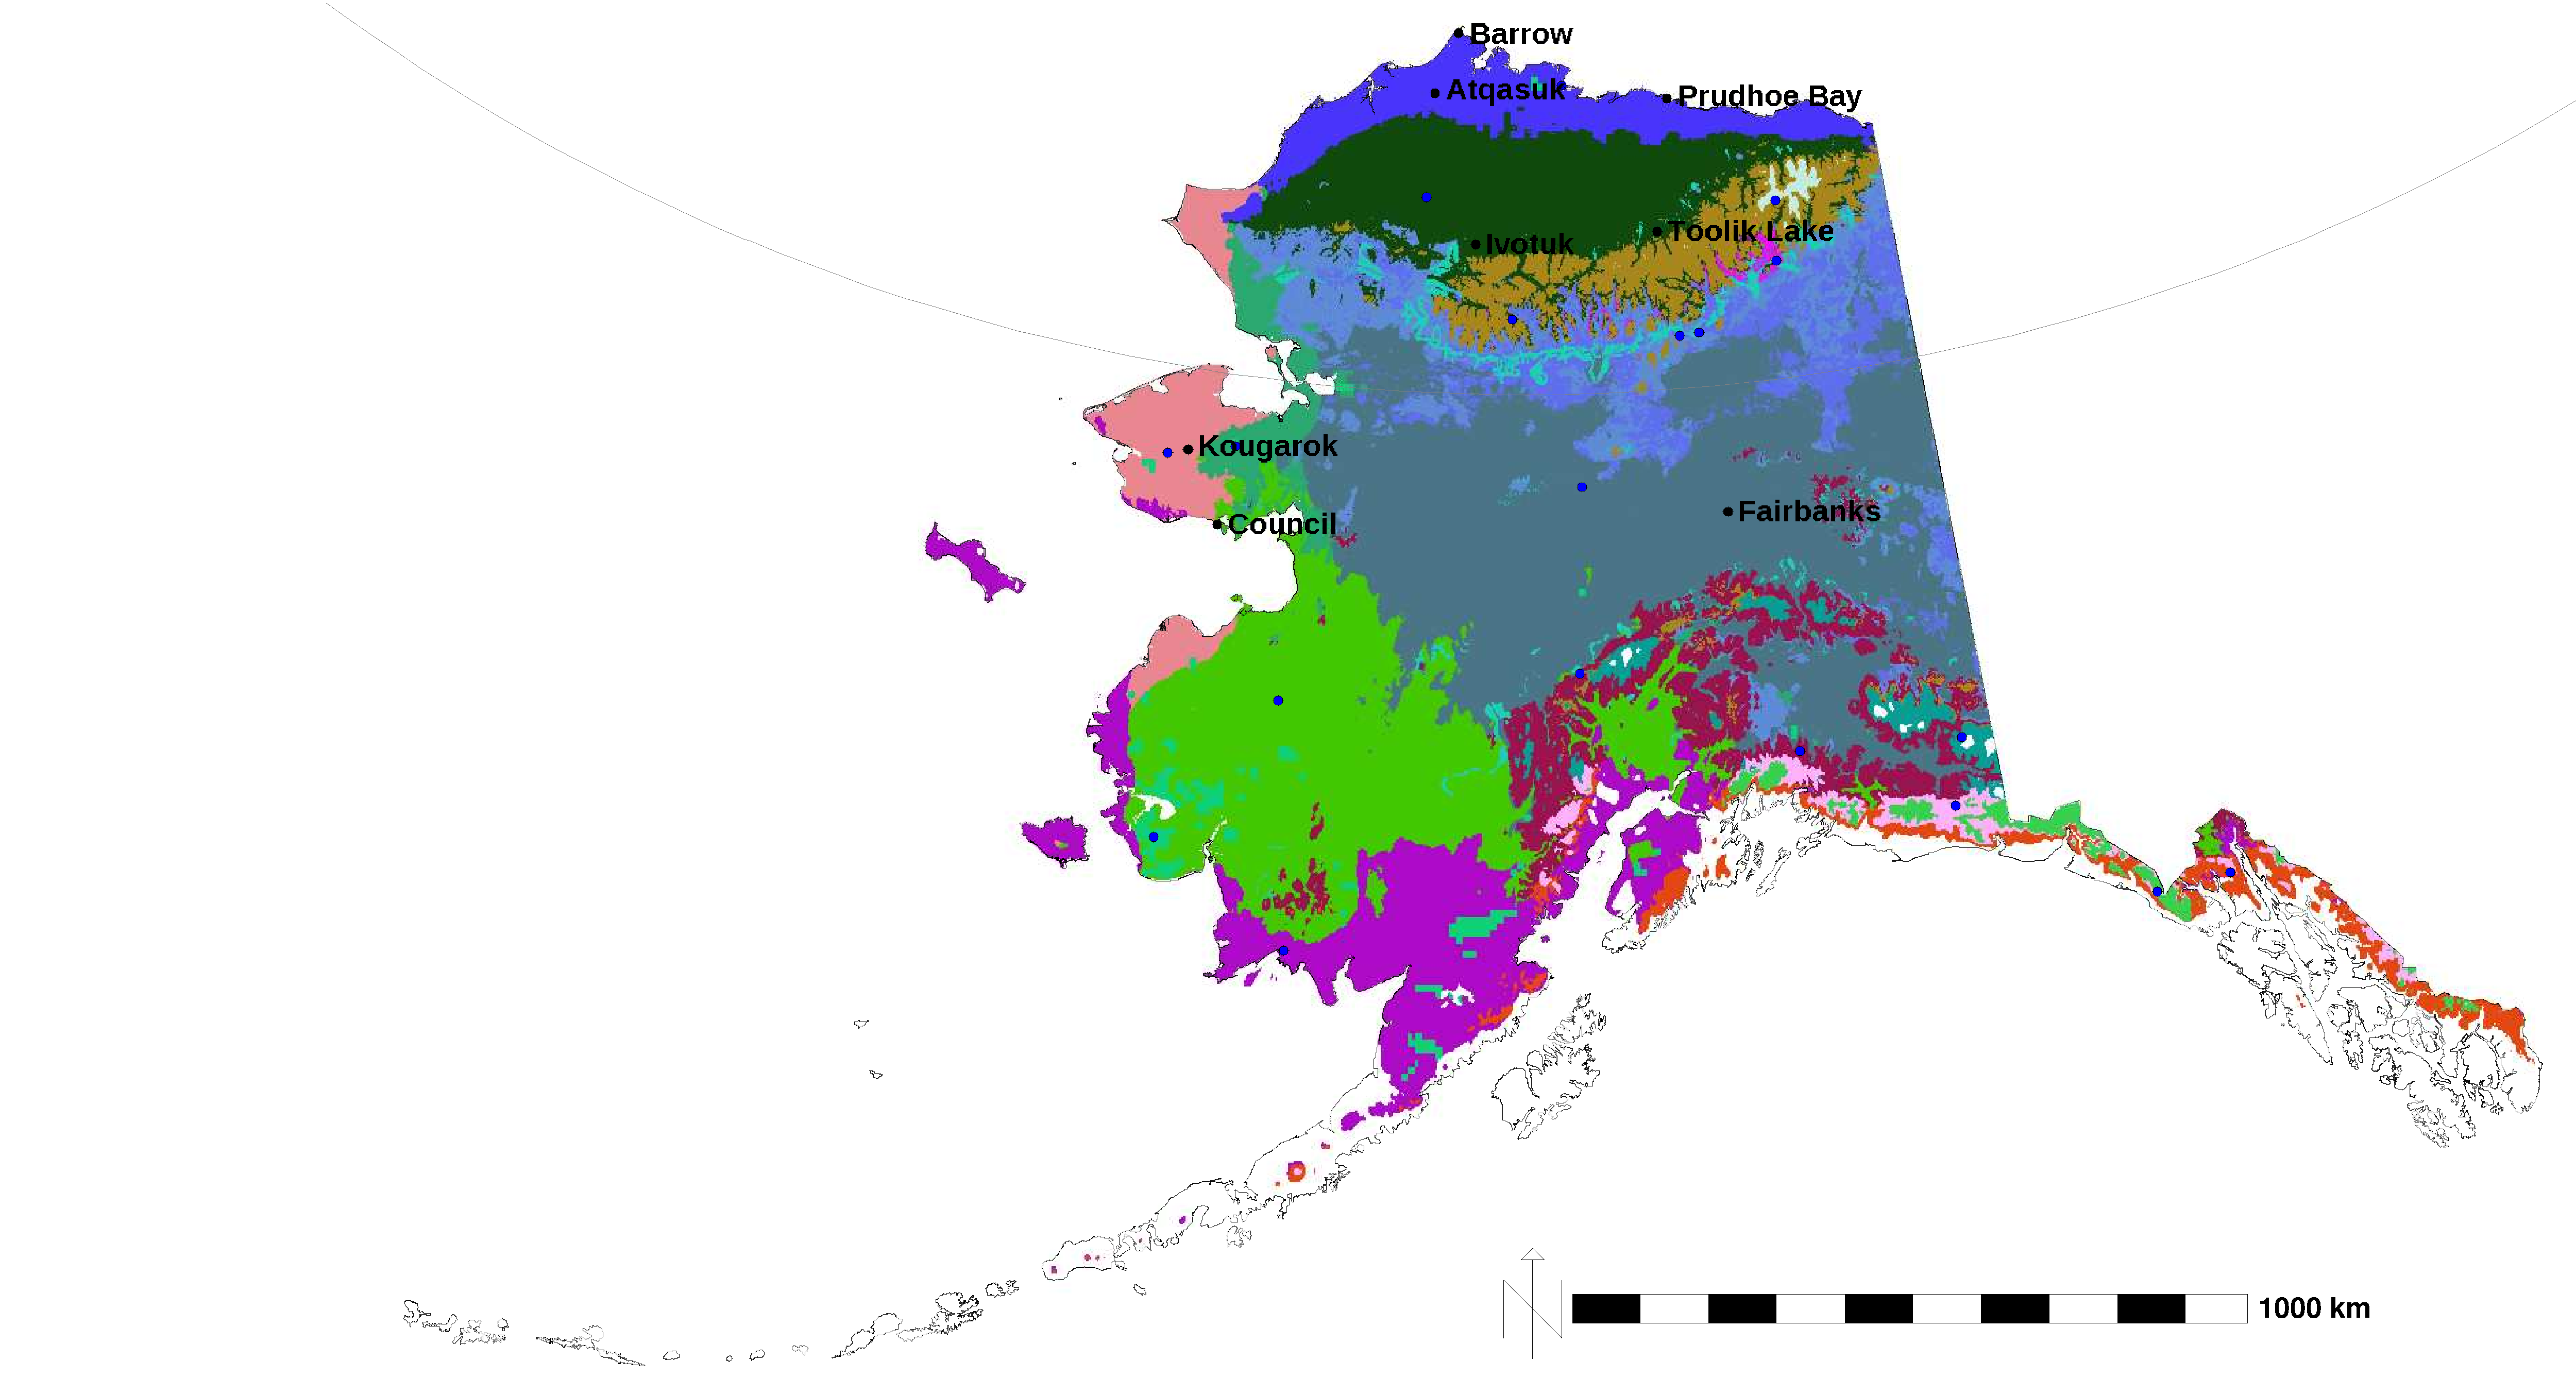
\includegraphics[width=0.50\textwidth]{ngee_figures/alaska_dem_Feb2012_20_2090-2099_barscale} \\
   2000--2009 & 2090--2099 \\
   \end{tabular}
  \vbox{\scriptsize\hfill\citep{Hoffman_LandscapeEcol_20131001}}
  %\caption{Cluster analysis.}
  \label{fig:alaska_both_20}
 \end{figure}
 \vskip-0.15in
\emph{Since the random colors are the same in both maps, a change in color
represents an environmental change between the present and the future.}

At this level of division, the two primary regions of the Seward
Peninsula and that of the northern boreal forest replace the two
regions on the North Slope almost entirely.

\end{frame}
%%%%%%%%%%%%%%%%%%%%%%%%%%%%%%%%%%%%%%%%%%%%%%%%%%%%%%%%%%%%%%%%%%%%%%%%%%%%%%%

%%%%%%%%%%%%%%%%%%%%%%%%%%%%%%%%%%%%%%%%%%%%%%%%%%%%%%%%%%%%%%%%%%%%%%%%%%%%%%%
\begin{frame}
 \frametitle{50 and 100 Alaska Ecoregions, Present}
 \vskip-0.15in
 \setlength{\tabcolsep}{0pt}
 \begin{figure}
   \begin{tabular}{cc}
   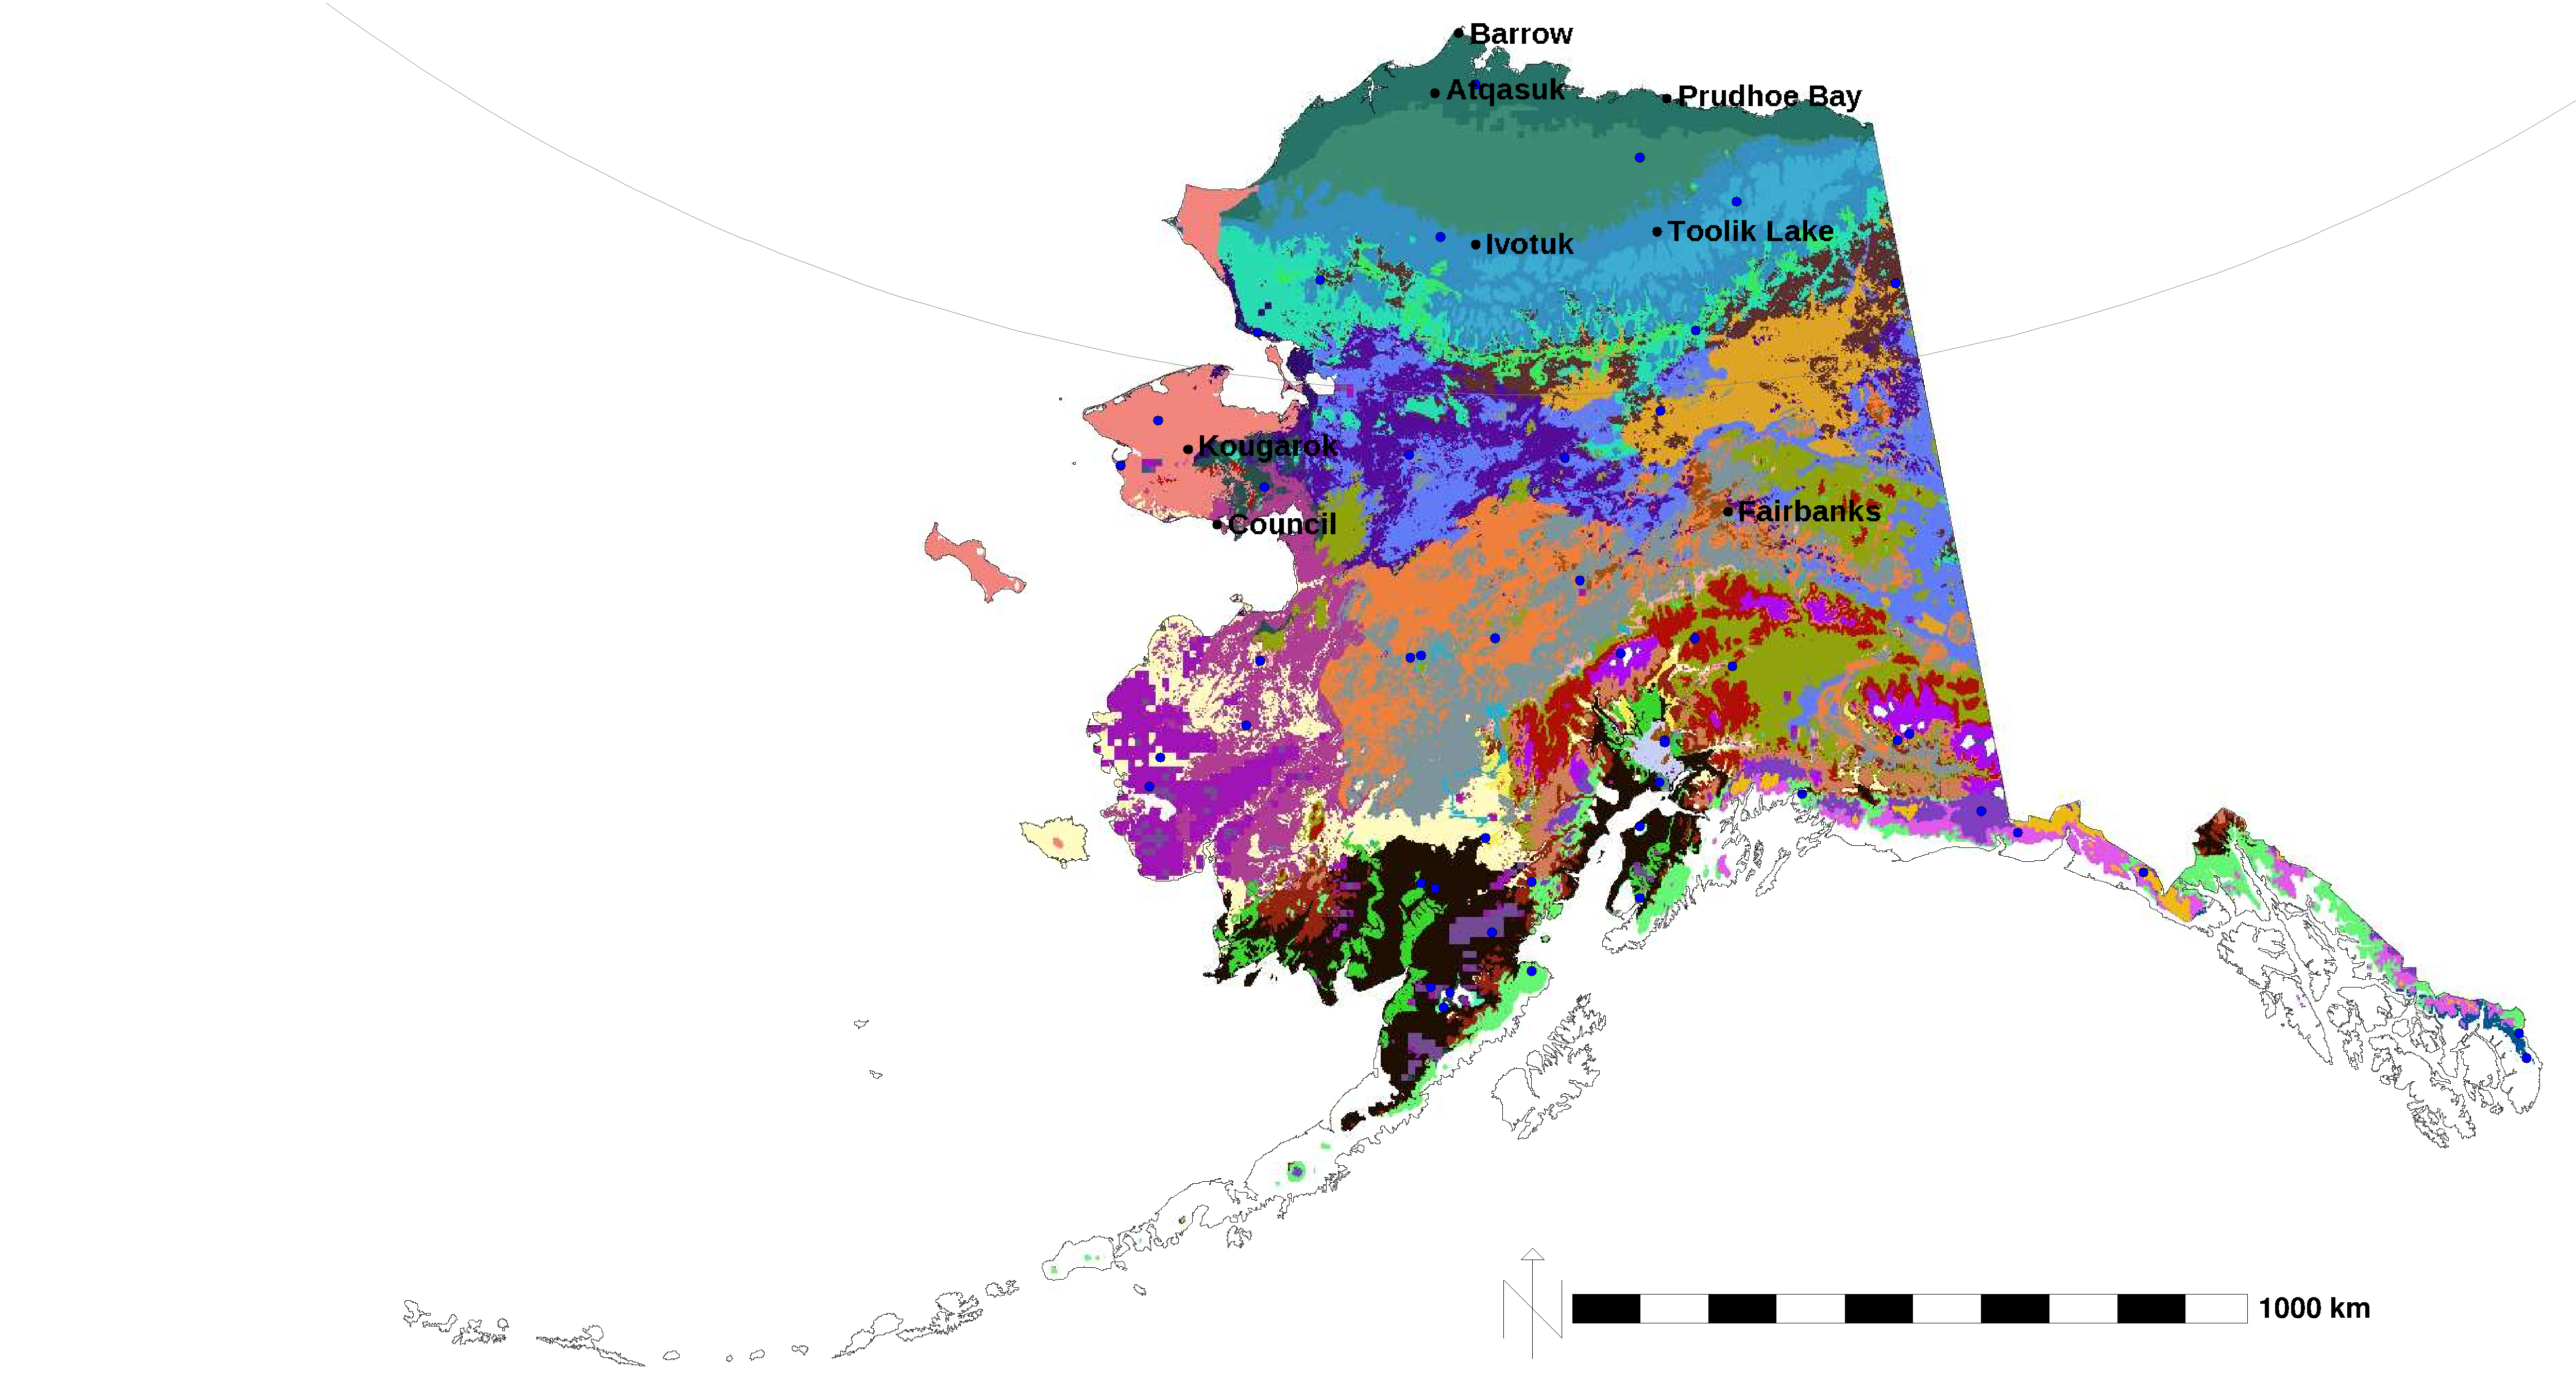
\includegraphics[width=0.50\textwidth]{ngee_figures/alaska_dem_Feb2012_50_2000-2009_barscale} &
   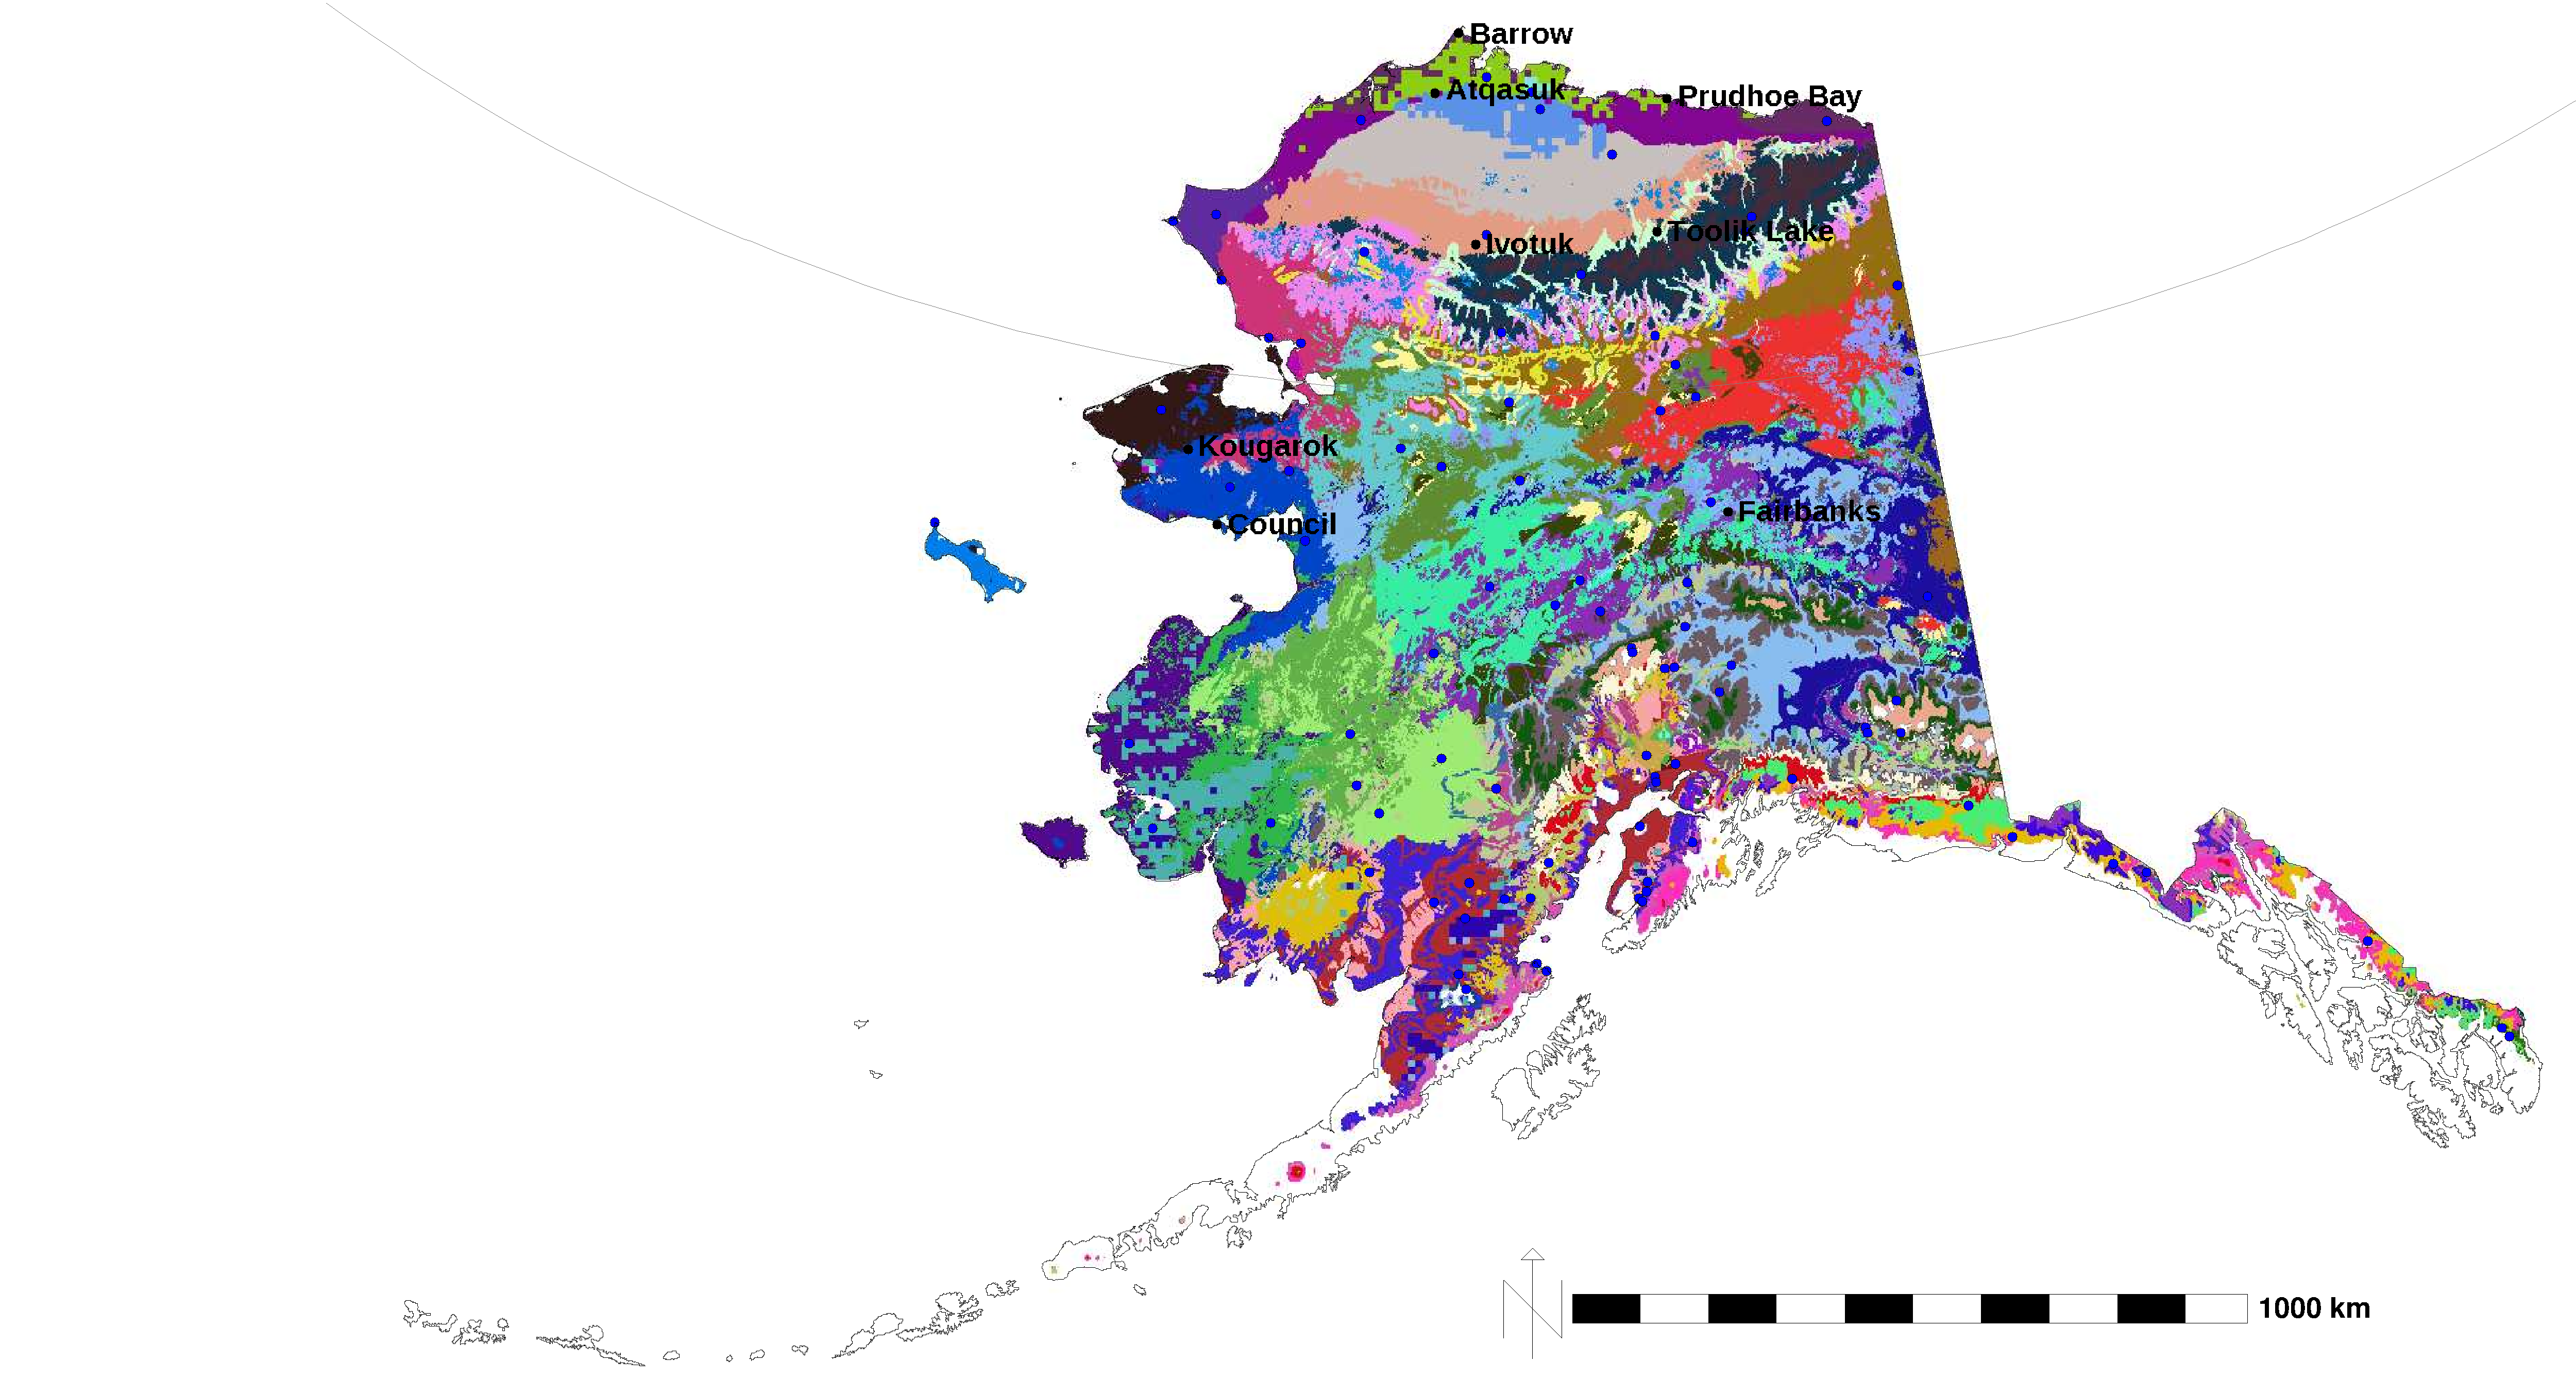
\includegraphics[width=0.50\textwidth]{ngee_figures/alaska_dem_Feb2012_100_2000-2009_barscale} \\
   $k=50$, 2000--2009 & $k=100$, 2000--2009 \\
   \end{tabular}
  \vbox{\scriptsize\hfill\citep{Hoffman_LandscapeEcol_20131001}}
  %\caption{Cluster analysis.}
  \label{fig:alaska_present_50_100}
 \end{figure}
 \vskip-0.15in
\emph{Since the random colors are the same in both maps, a change in color
represents an environmental change between the present and the future.}\\

At high levels of division, some regions vanish between the present
and future while other region representing new combinations of
environmental conditions come into existence.

\end{frame}
%%%%%%%%%%%%%%%%%%%%%%%%%%%%%%%%%%%%%%%%%%%%%%%%%%%%%%%%%%%%%%%%%%%%%%%%%%%%%%%

%%%%%%%%%%%%%%%%%%%%%%%%%%%%%%%%%%%%%%%%%%%%%%%%%%%%%%%%%%%%%%%%%%%%%%%%%%%
% Hierarchical ecoregions
%%%%%%%%%%%%%%%%%%%%%%%%%%%%%%%%%%%%%%%%%%%%%%%%%%%%%%%%%%%%%%%%%%%%%%%%%%%
%\begin{frame}
% \frametitle{A Hierarchy of Ecoregions}
% %\vbox{\centering\large\textbf{\color{blue}A Hierarchy of Ecoregions}}
% \vskip-0.15in
%\begin{figure}\scriptsize
%  \subfigure[\scriptsize At $k = 10$, the North Slope is occupied by
%Ecoregion \#3, which corresponds to the Arctic Tundra Level 2 ecological
%group.]{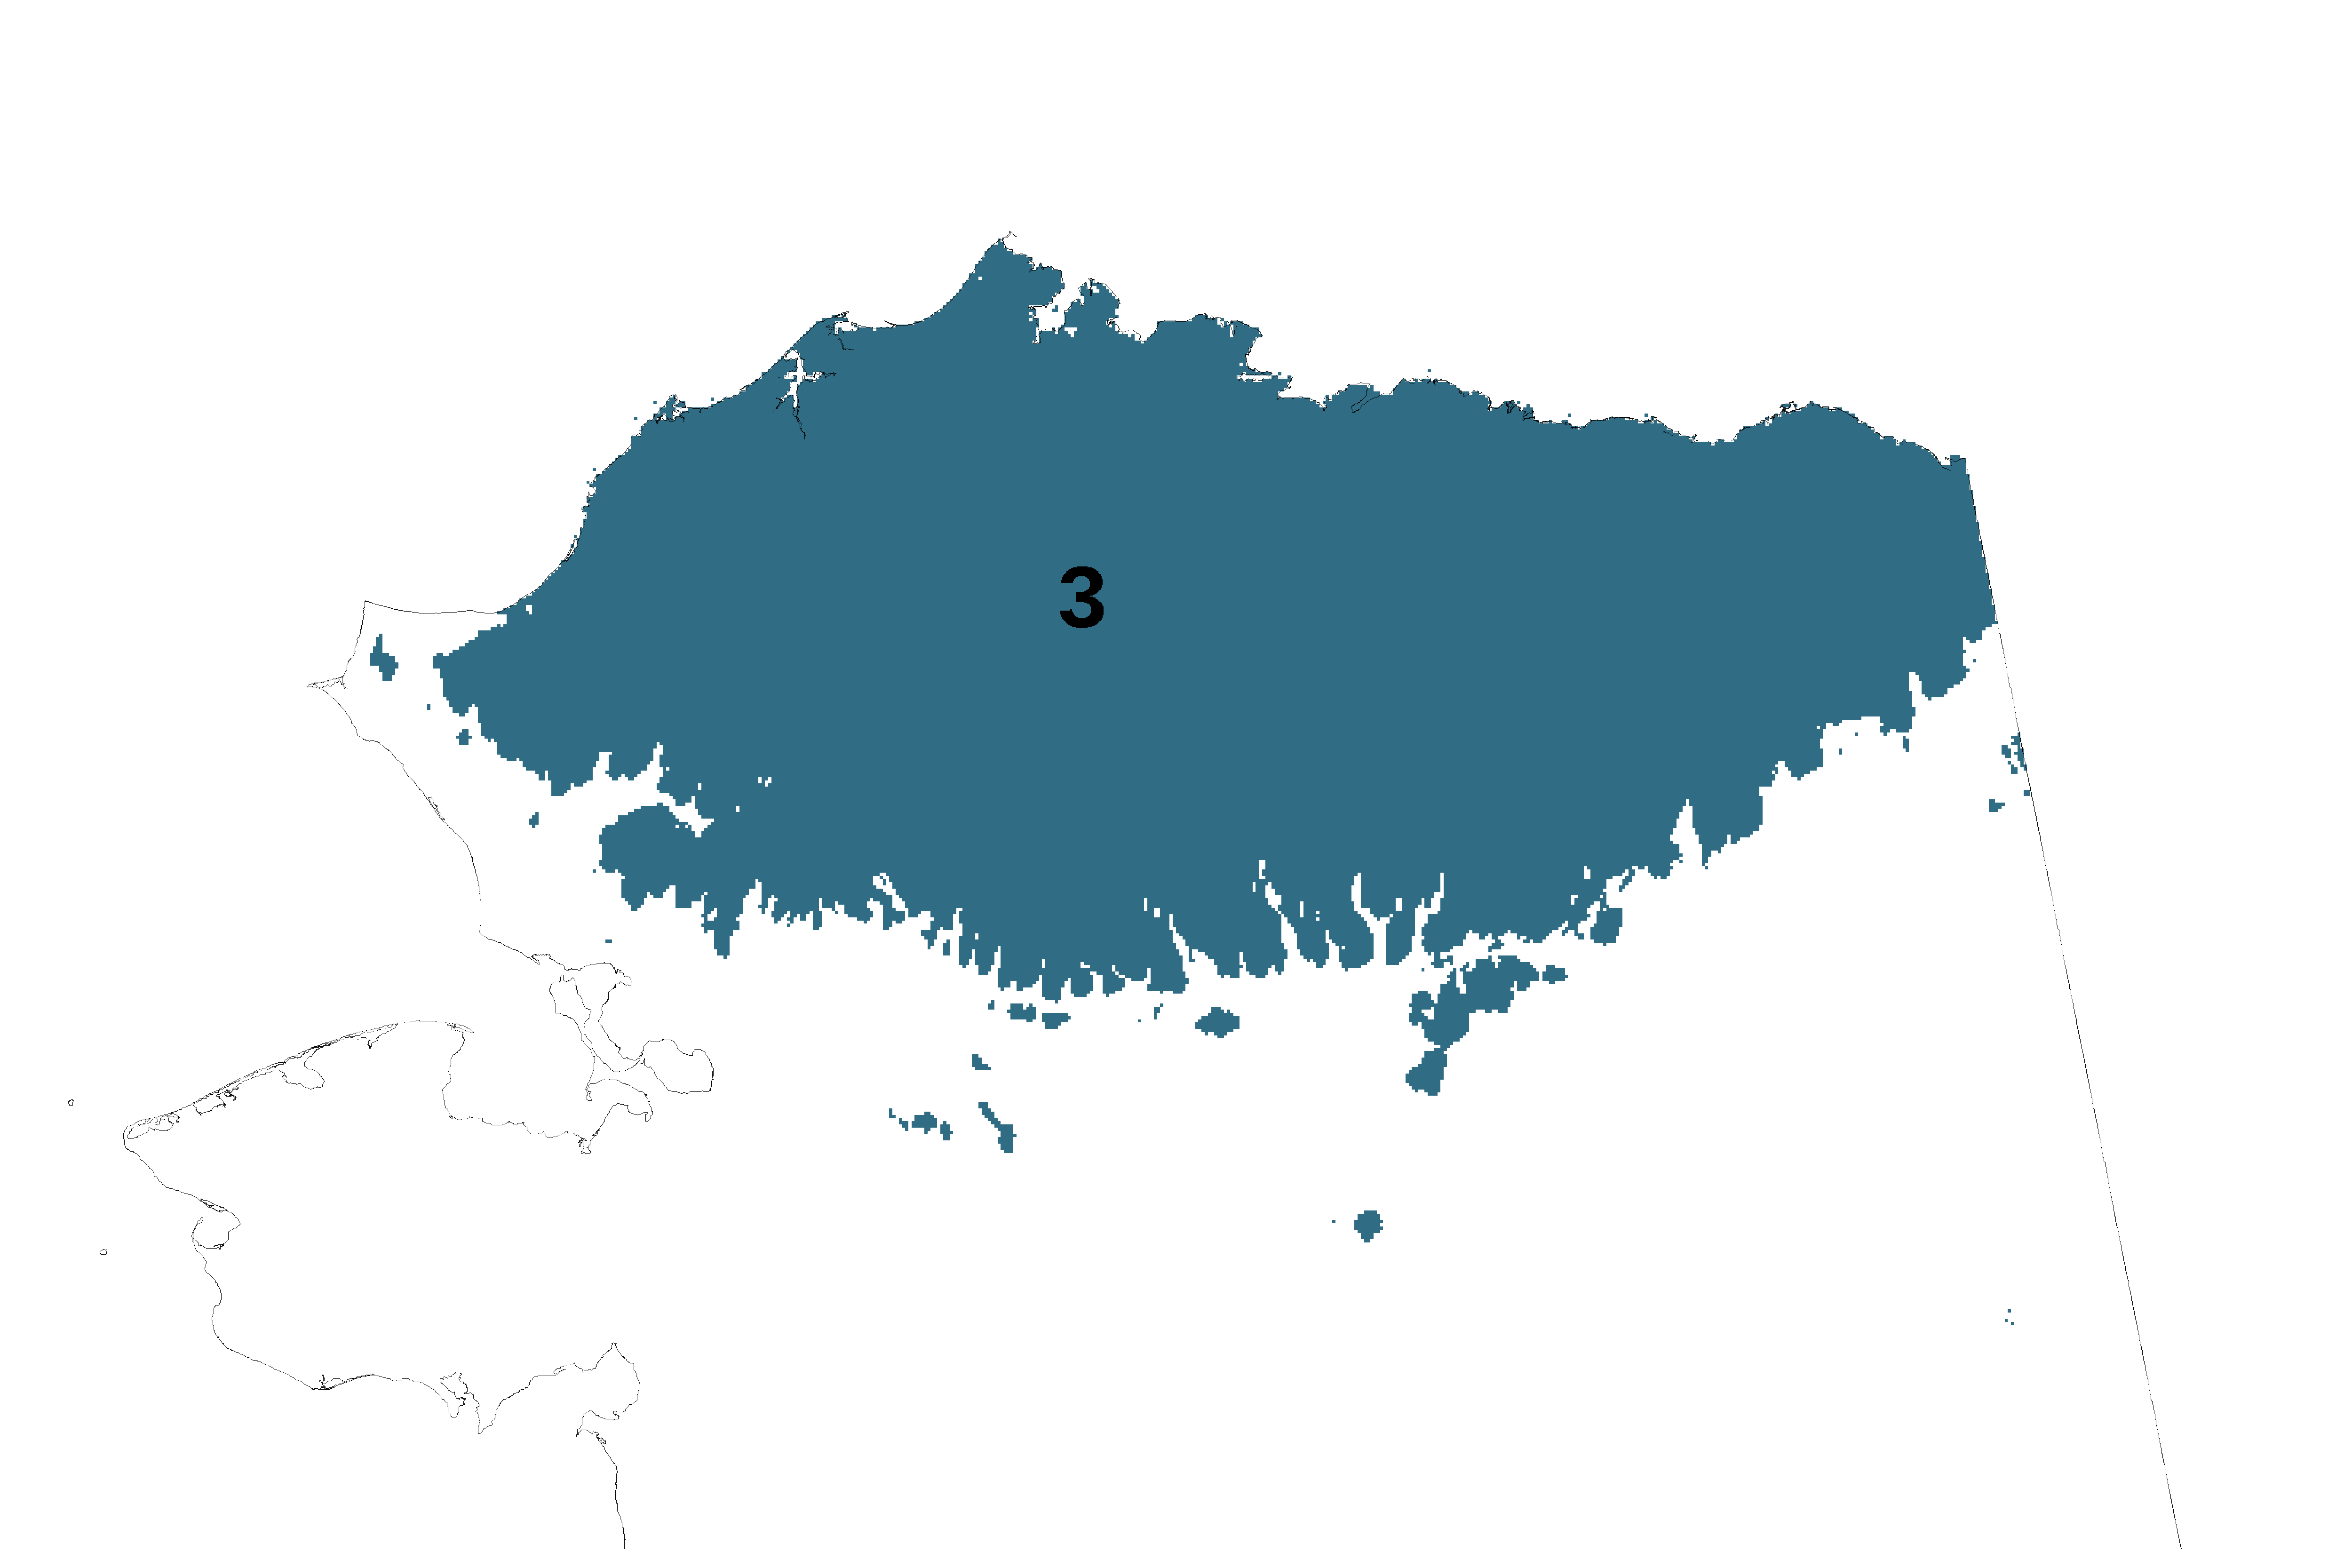
\includegraphics[width=0.315\textwidth]{ngee_figures/arctic_tundra_k10.pdf}\label{fig:k10_NSA}} \hfill
%   \subfigure[\scriptsize At $k = 20$, the North Slope is occupied by 
%Ecoregion \#5, corresponding to the Brooks Range ecoregion; and 
%Ecoregion \#13, corresponding to the Beaufort Coastal Plains
%ecoregion.]{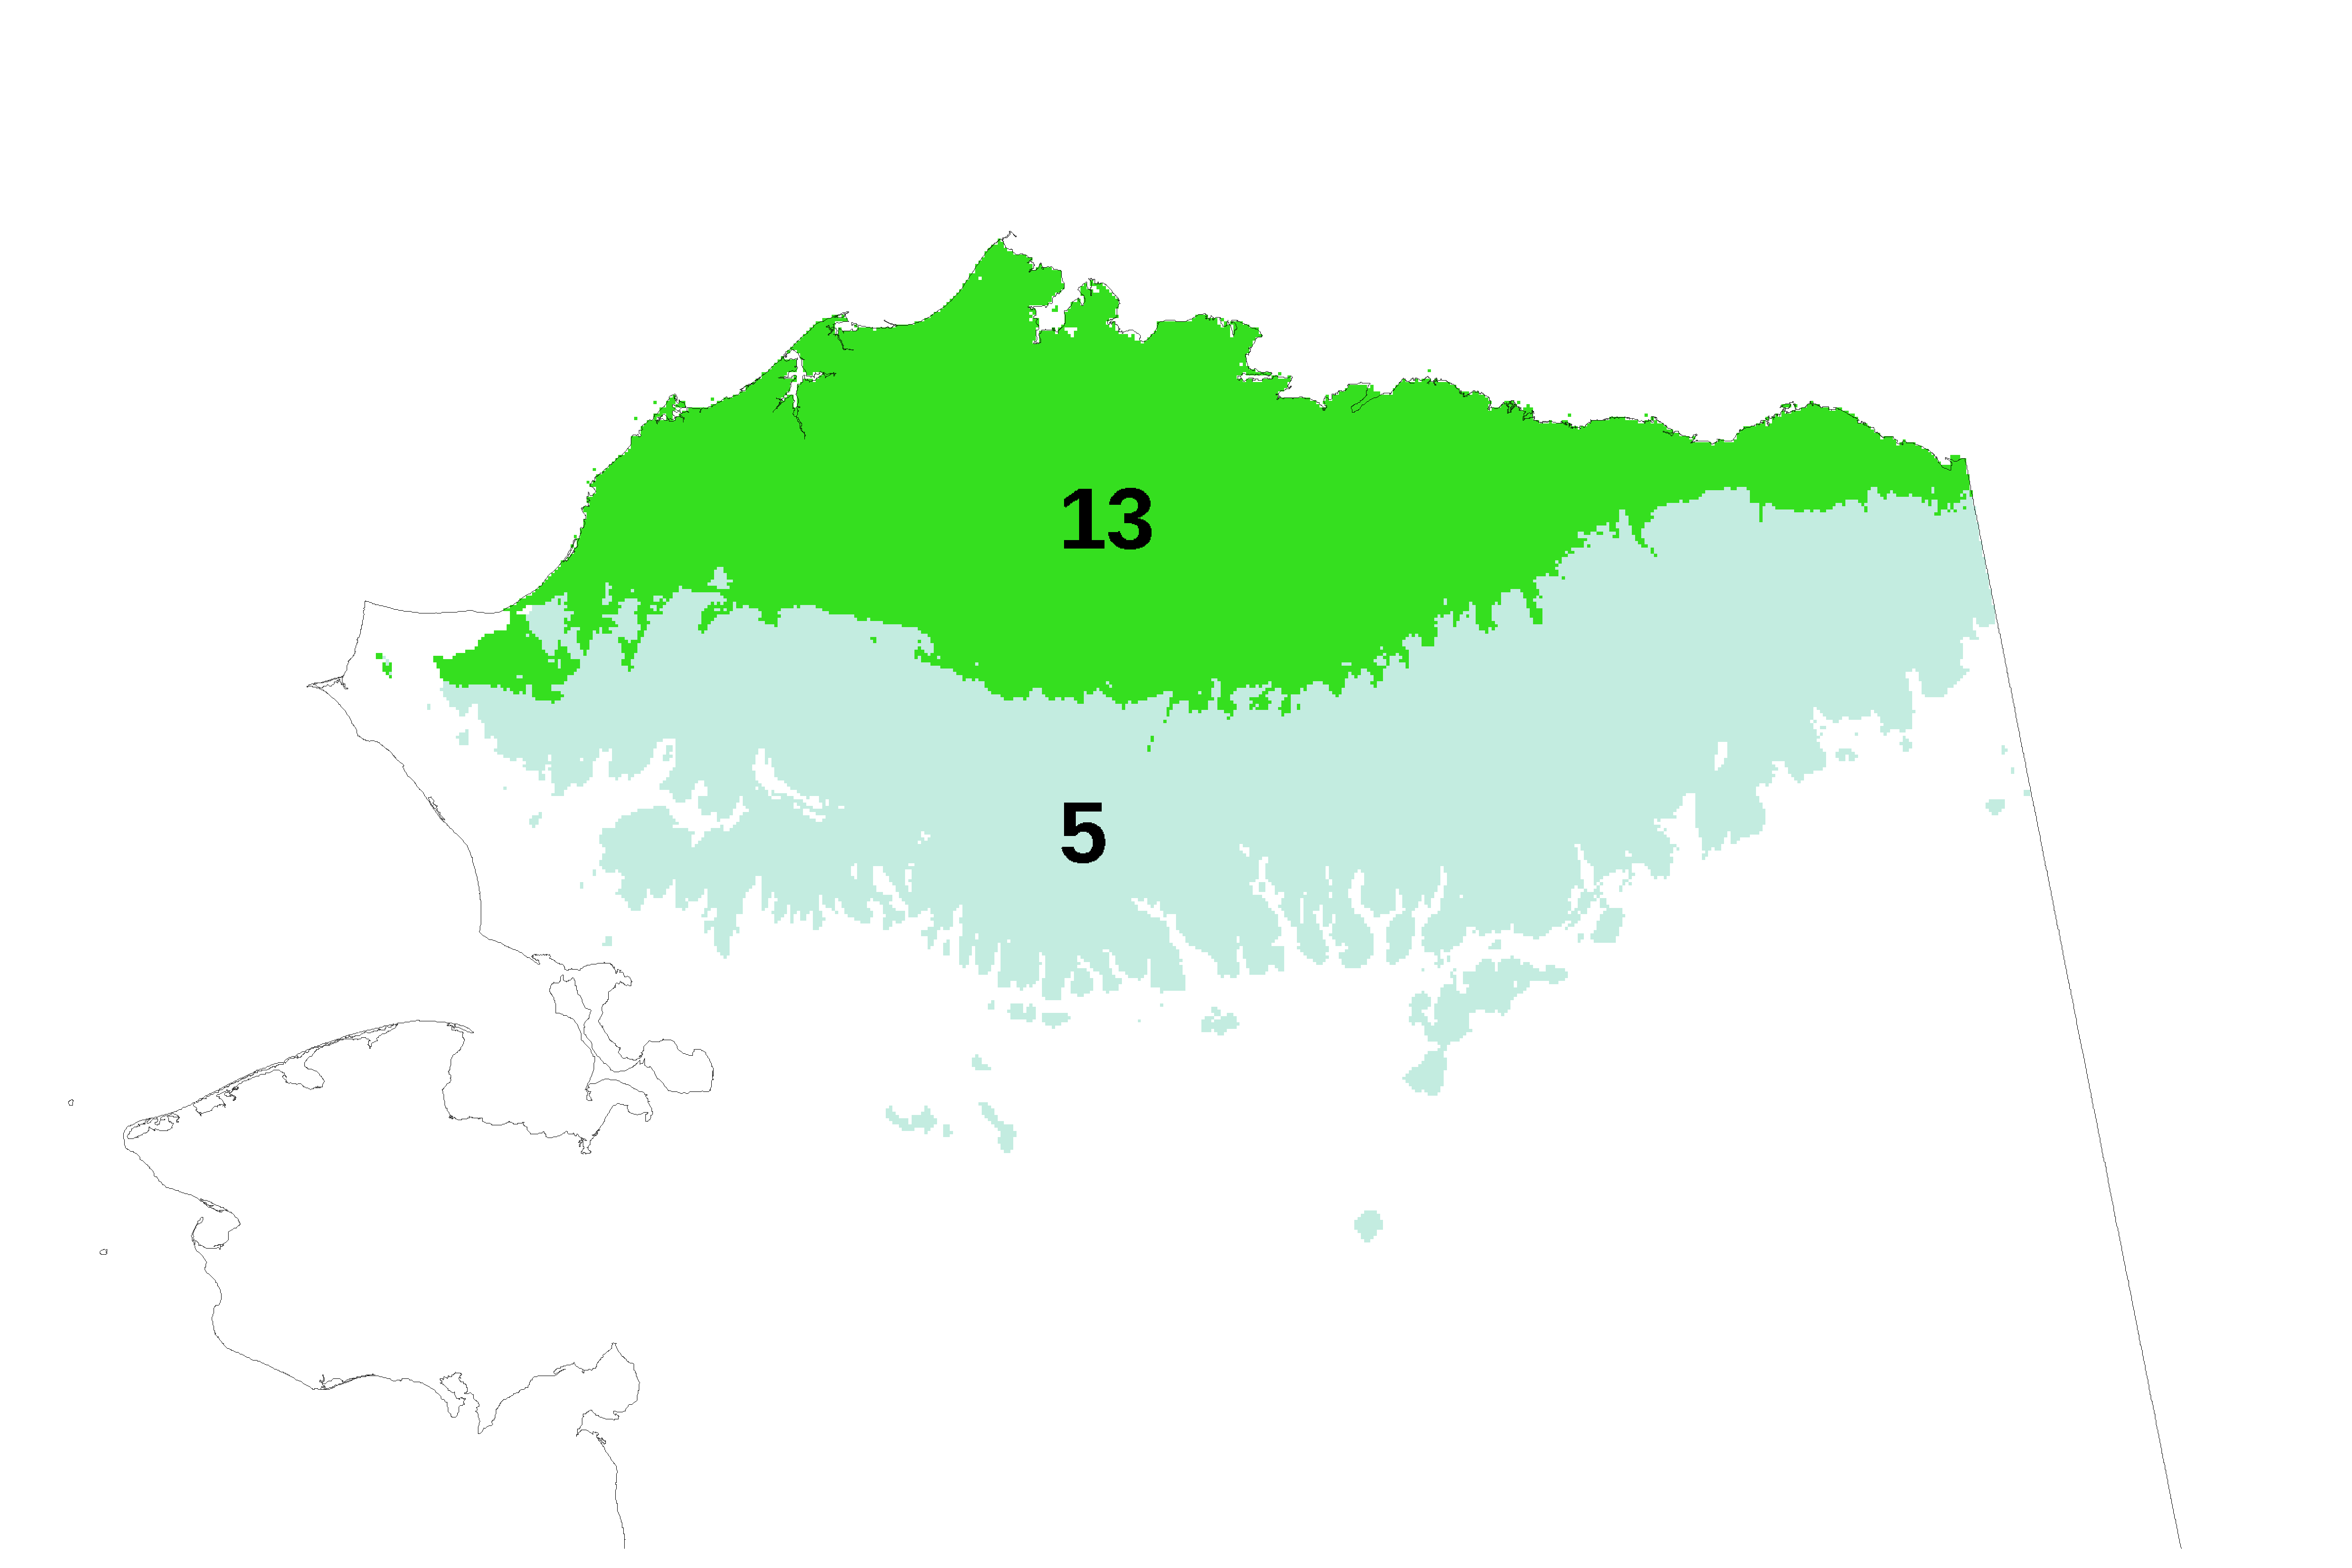
\includegraphics[width=0.315\textwidth]{ngee_figures/arctic_tundra_k20.pdf}\label{fig:k20_NSA}} \hfill
%   \subfigure[\scriptsize At $k = 50$, the North Slope is occupied by 
%Ecoregion \#32, corresponding to the Intermontane Boreal ecological group;
%Ecoregions \#33 and \#34, corresponding to mid- and high-elevation
%of the Brooks Range ecoregion; Ecoregion \#35,
%corresponding to the Brooks Foothills ecoregion; and Ecoregion \#40,
%corresponding to the Beaufort Coastal Plains
%ecoregion.]{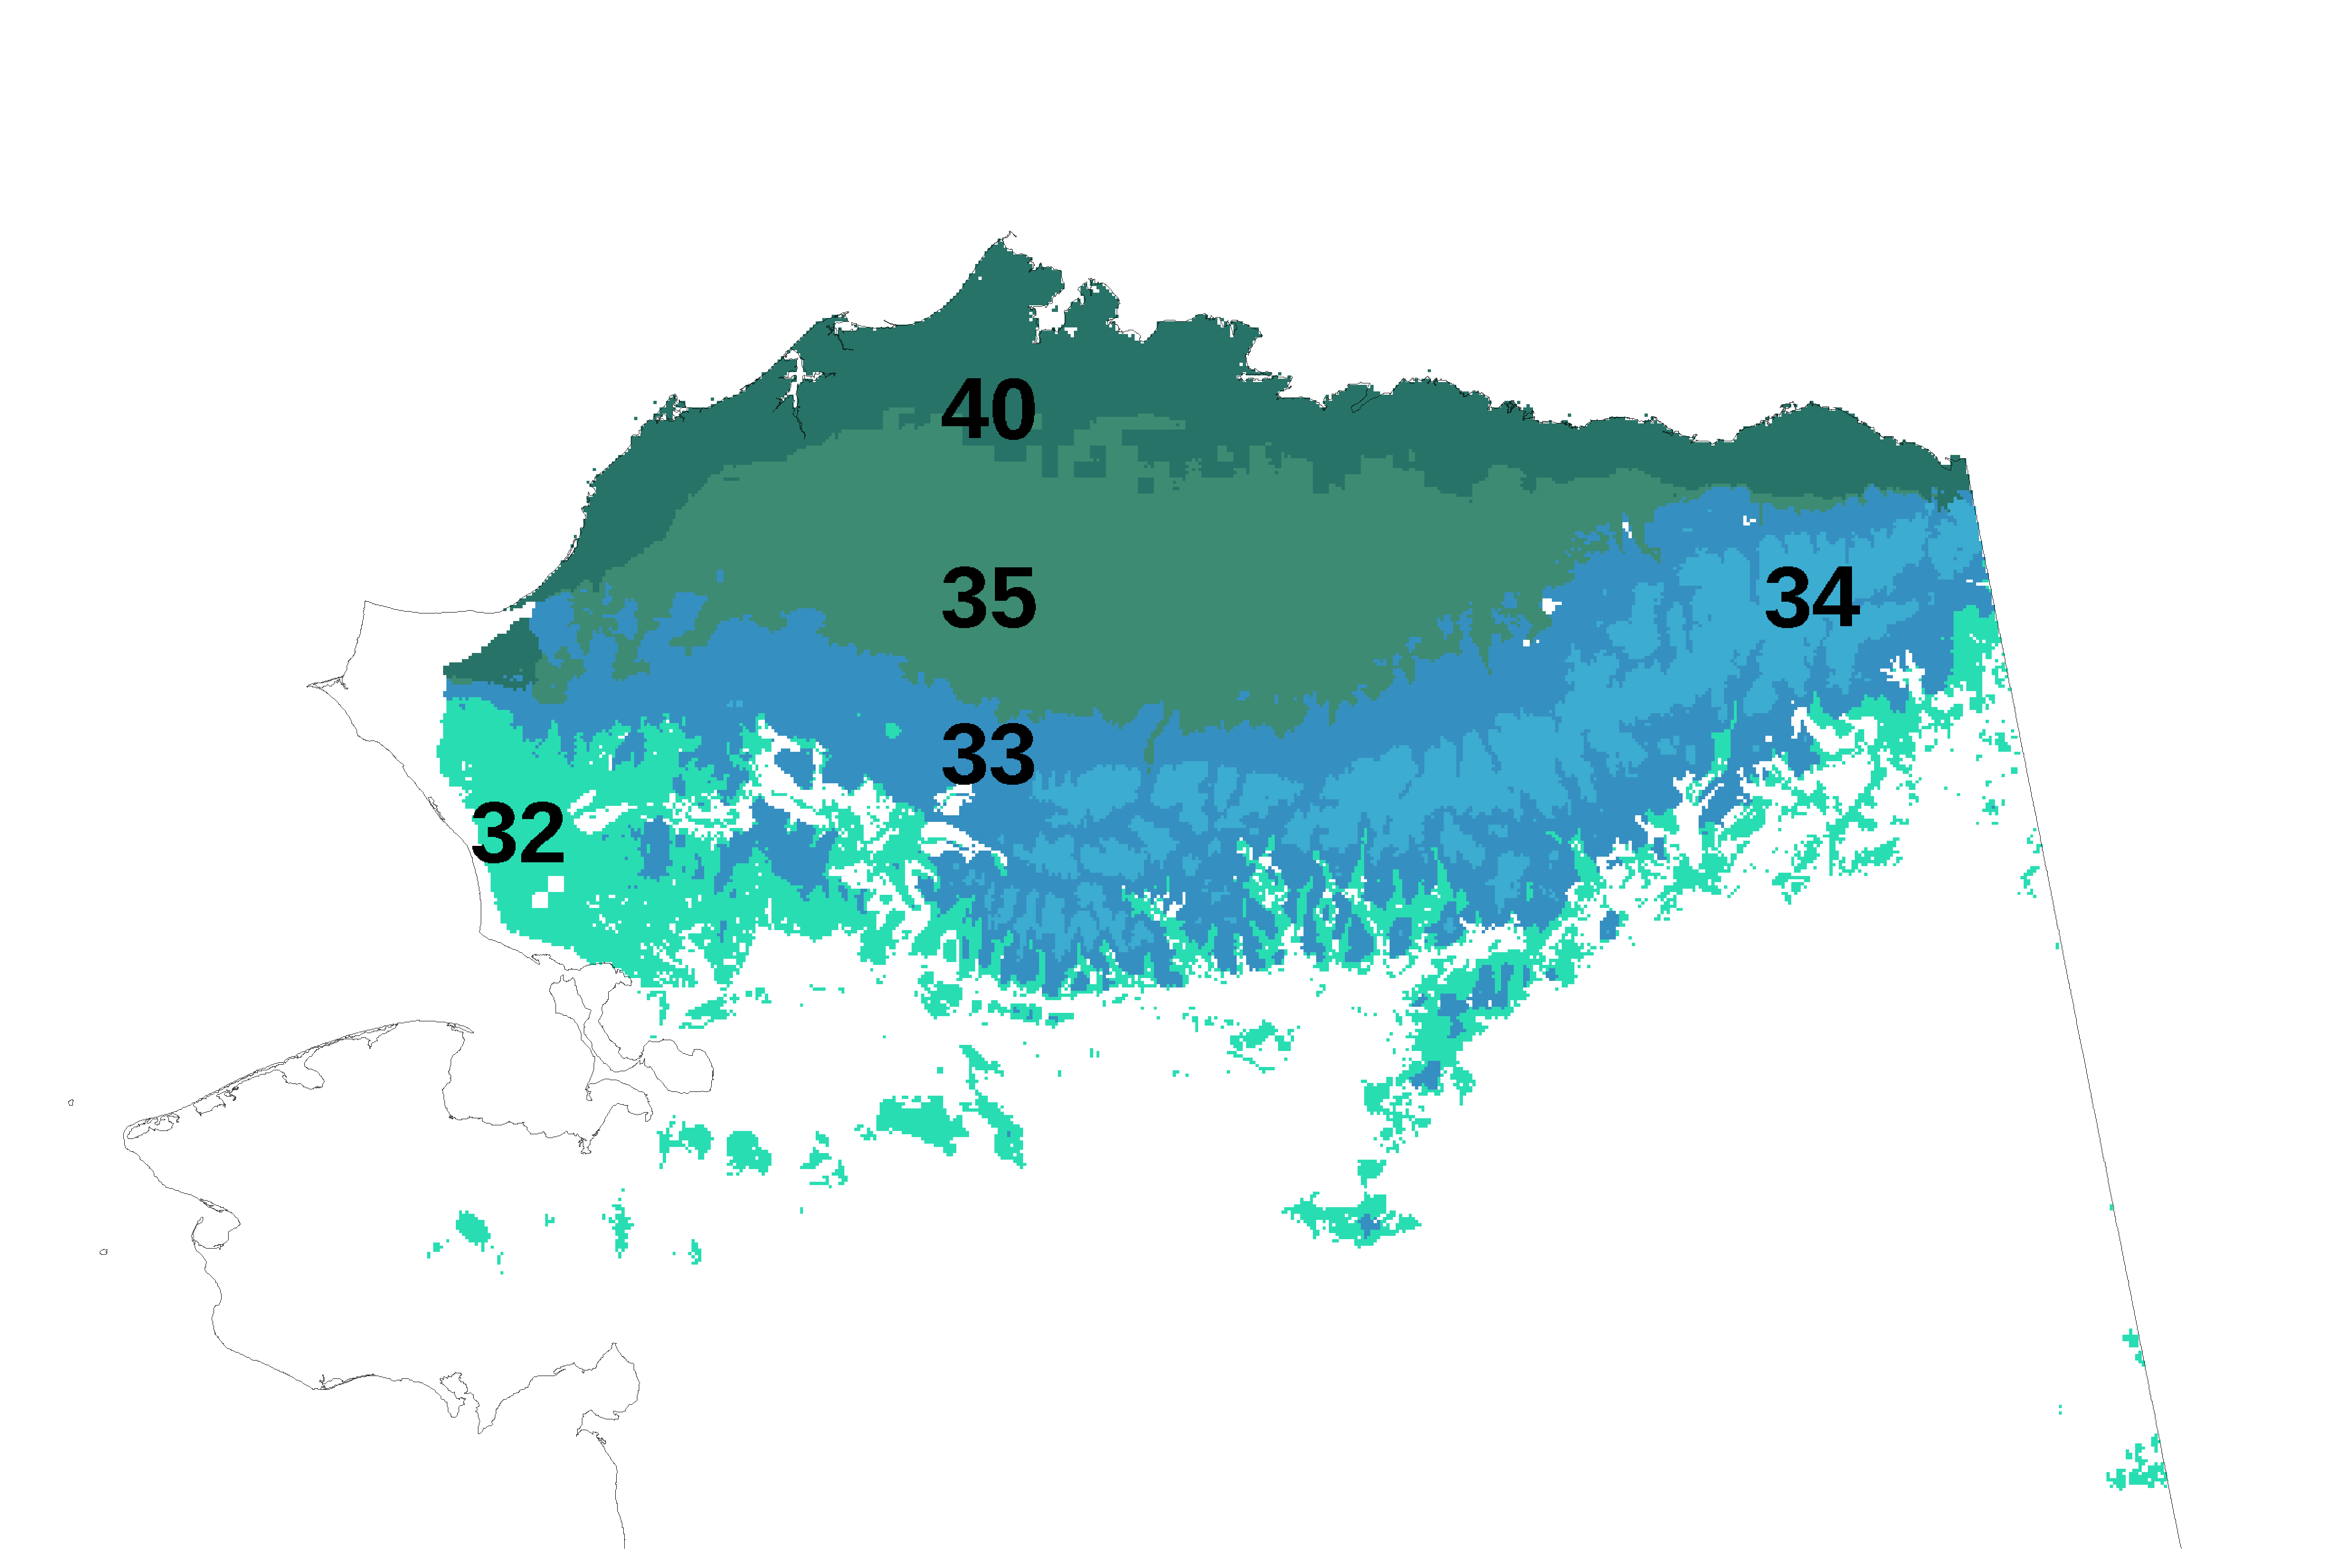
\includegraphics[width=0.315\textwidth]{ngee_figures/arctic_tundra_k50.pdf}\label{fig:k50_NSA}}
%%  \caption{\tiny A hierarchy of increasingly specific ecoregions for the
%% North Slope of Alaska emerge by increasing the level of division in the
%% MSTC algorithm.  MSTC cluster numbers are shown and the spatially
%% corresponding Level 2 ecological group or ecoregion defined by
%% \citet{Nowacki2001} is identified.}
%  \label{fig:k10+20+50_NSA}
%\end{figure}
%\end{frame}
%%%%%%%%%%%%%%%%%%%%%%%%%%%%%%%%%%%%%%%%%%%%%%%%%%%%%%%%%%%%%%%%%%%%%%%%%%%

\subsection[Representativeness]{Representativeness Analysis}

%%%%%%%%%%%%%%%%%%%%%%%%%%%%%%%%%%%%%%%%%%%%%%%%%%%%%%%%%%%%%%%%%%%%%%%%%%%%%%%
\begin{frame}
 \frametitle{NGEE Arctic Site Representativeness}
 \begin{itemize}
  \item This representativeness analysis uses the standardized
$n$-dimensional data space formed from all input data layers.
  \item In this data space, the Euclidean distance between a sampling
location (like Barrow) and every other point is calculated.
  \item These data space distances are then used to generate
grayscale maps showing the similarity, or lack thereof, of every
location to the sampling location.
  \item In the subsequent maps, white areas are well represented by
the sampling location or network, while dark and black areas
as poorly represented by the sampling location or network.
  \item This analysis assumes that the climate surrogates maintain
their predictive power and that no significant biological
adaptation occurs in the future.
 \end{itemize}
\end{frame}
%%%%%%%%%%%%%%%%%%%%%%%%%%%%%%%%%%%%%%%%%%%%%%%%%%%%%%%%%%%%%%%%%%%%%%%%%%%%%%%

%%%%%%%%%%%%%%%%%%%%%%%%%%%%%%%%%%%%%%%%%%%%%%%%%%%%%%%%%%%%%%%%%%%%%%%%%%%%%%%
\begin{frame}
 \frametitle{Present Representativeness of Barrow or ``Barrow-ness''}

 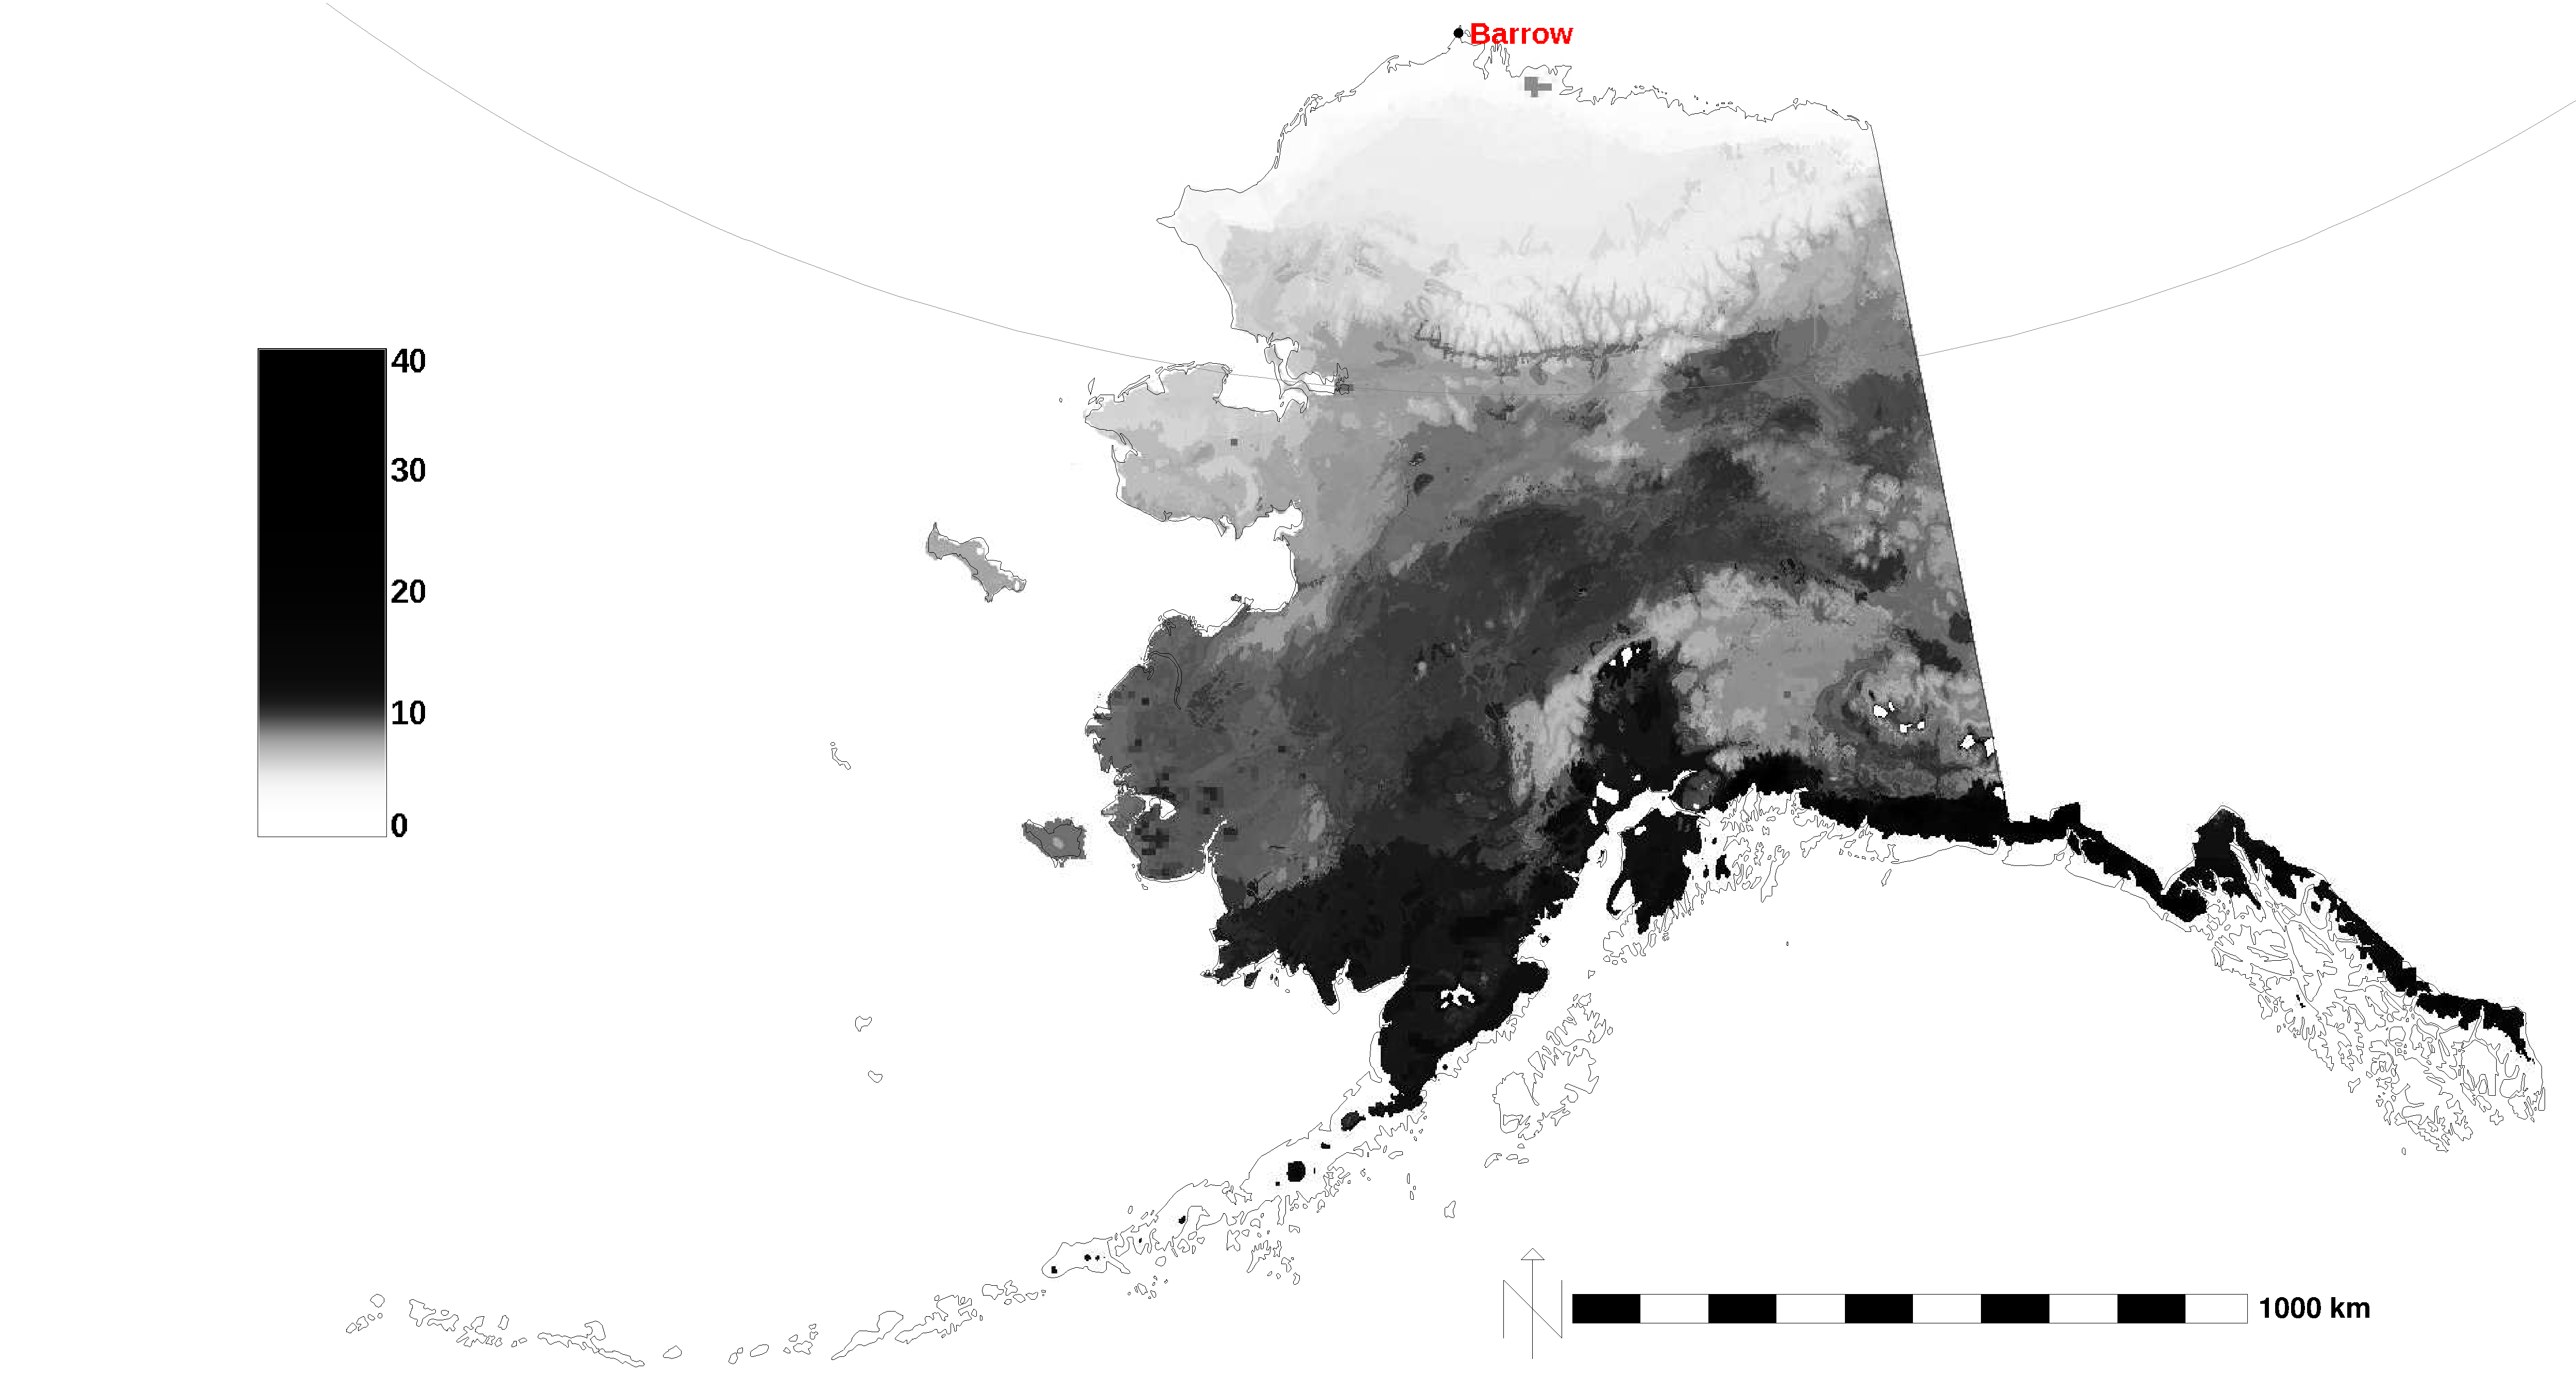
\includegraphics[width=\textwidth]{ngee_figures/alaska_2000_2009_dem_Feb2012_k1000ness_1sites.pdf} \\
  \vbox{\scriptsize\hfill\citep{Hoffman_LandscapeEcol_20131001}}
\medskip
Light-colored regions are well represented and dark-colored regions are
poorly represented by the sampling location listed in \textbf{\color{red}red}.

\end{frame}
%%%%%%%%%%%%%%%%%%%%%%%%%%%%%%%%%%%%%%%%%%%%%%%%%%%%%%%%%%%%%%%%%%%%%%%%%%%%%%%
%\begin{frame}
% \frametitle{Present vs. Future Barrow-ness}
% \vskip-0.15in
% \setlength{\tabcolsep}{0pt}
% \begin{figure}
%   \begin{tabular}{cc}
%   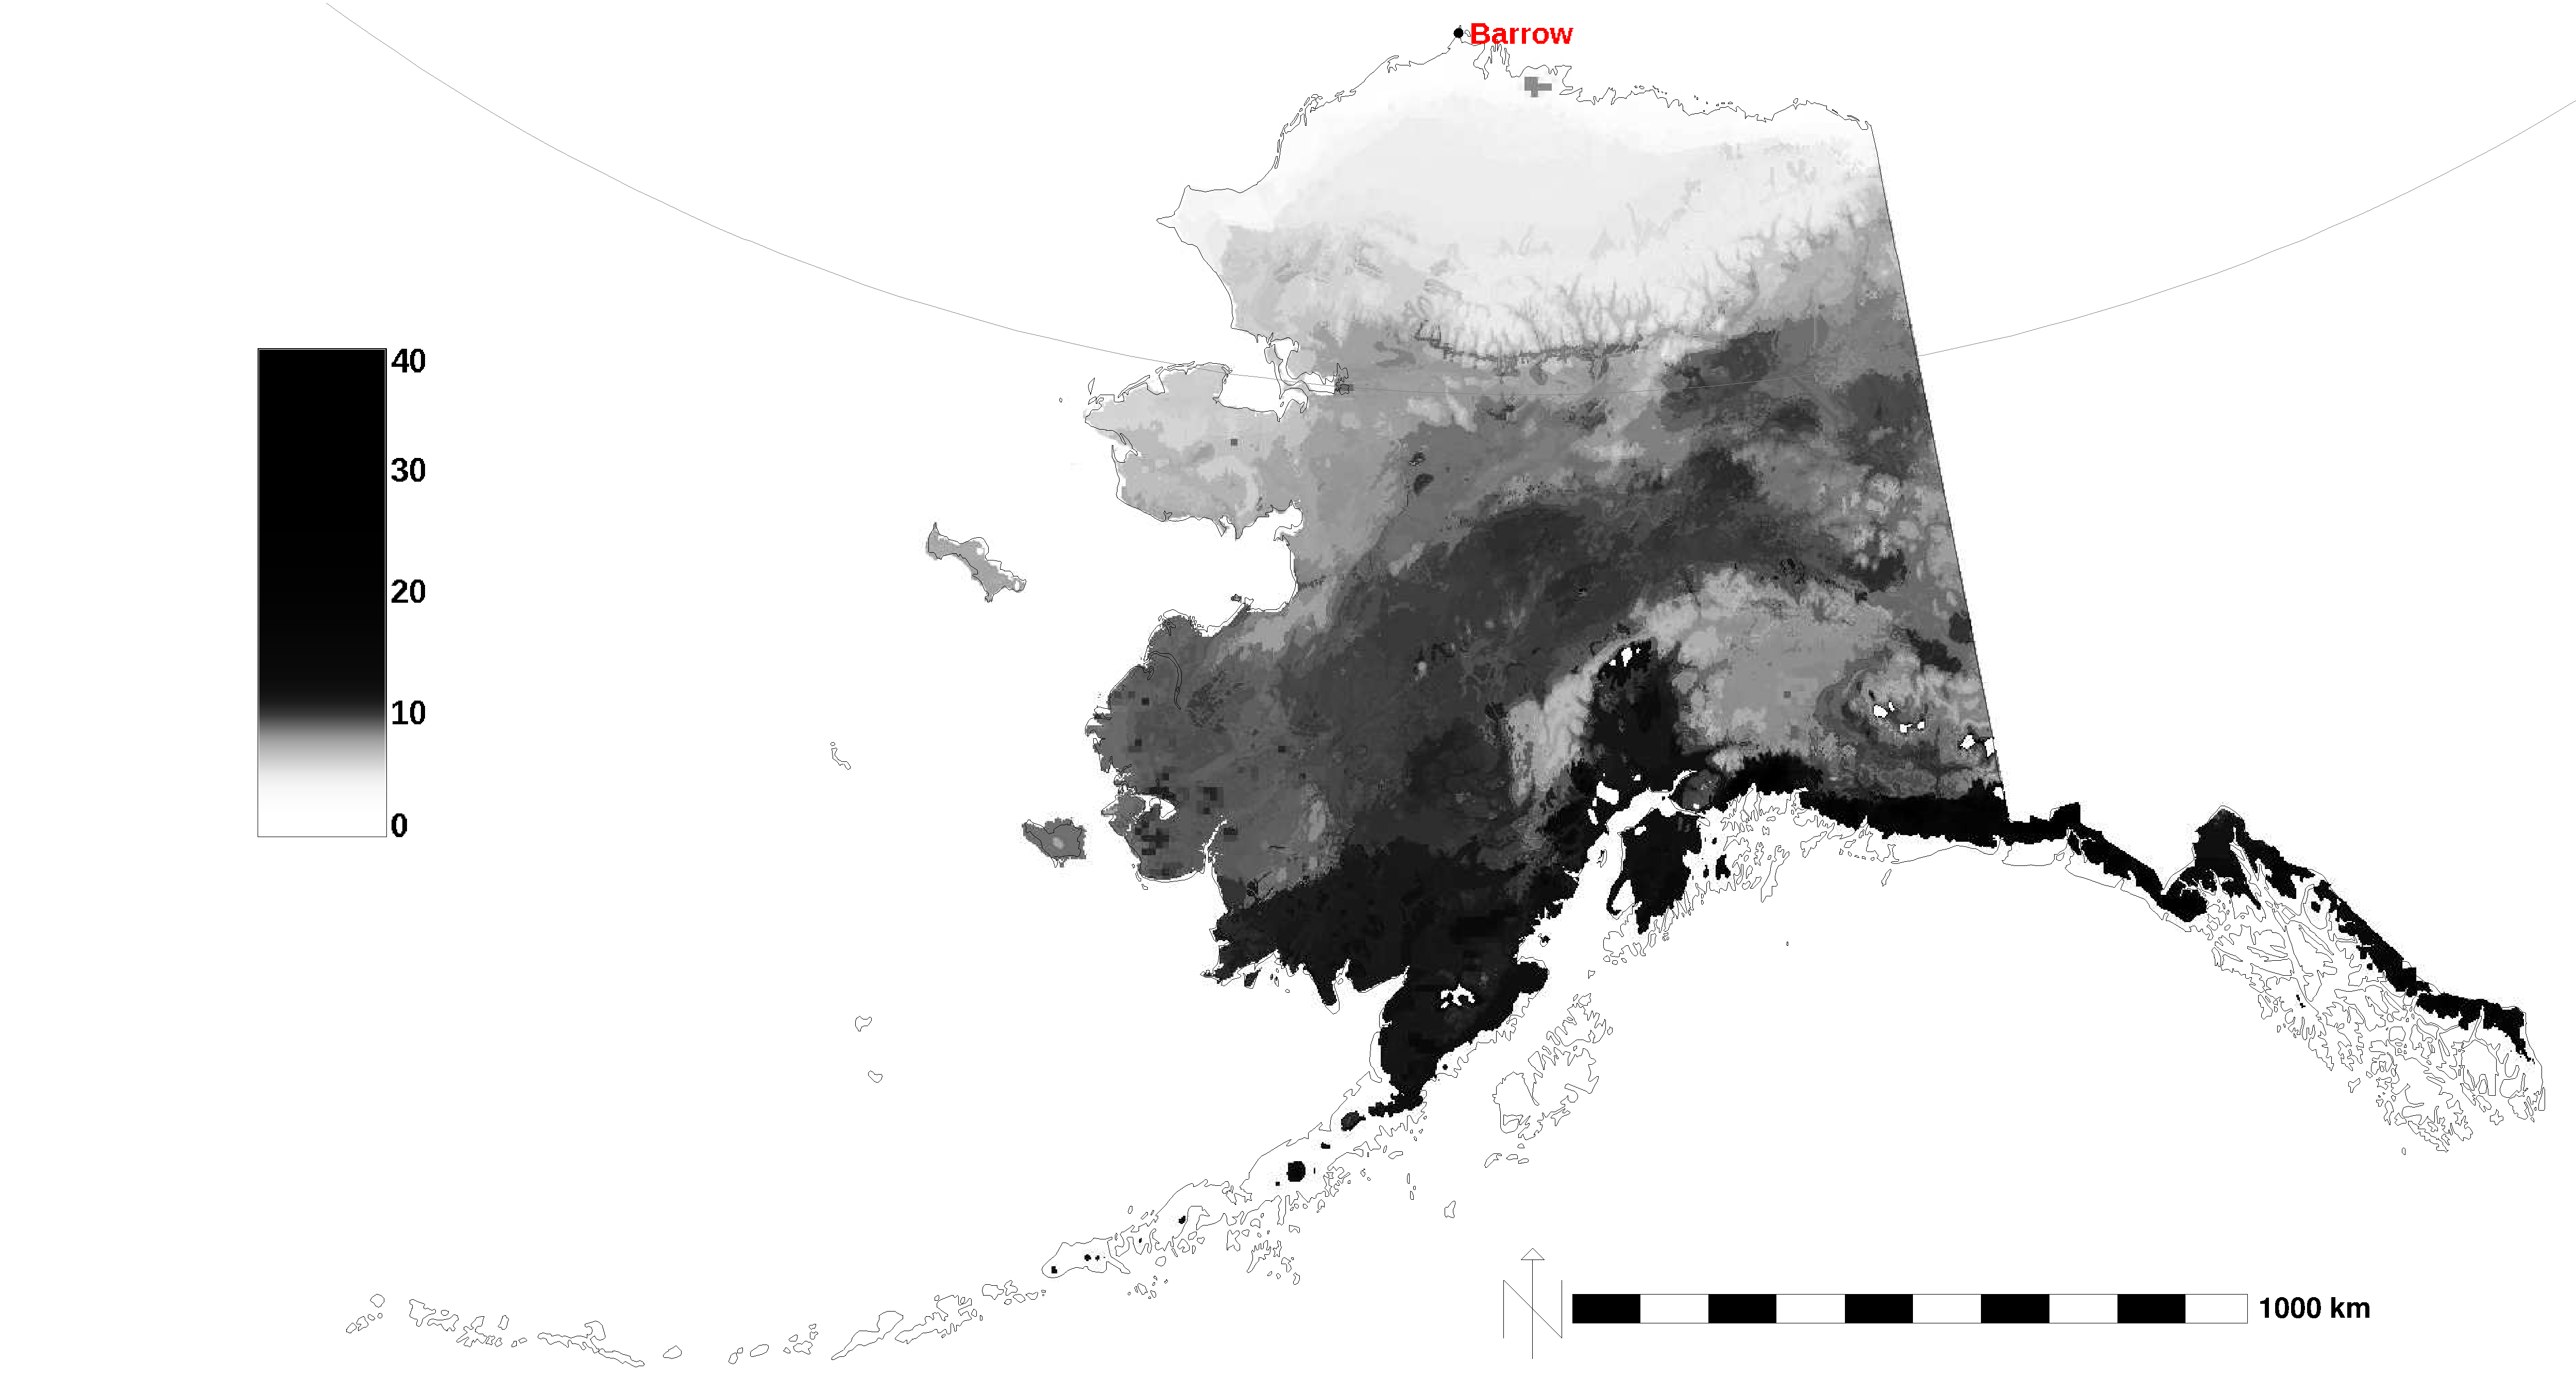
\includegraphics[width=0.50\textwidth]{ngee_figures/alaska_2000_2009_dem_Feb2012_k1000ness_1sites.pdf} &
%   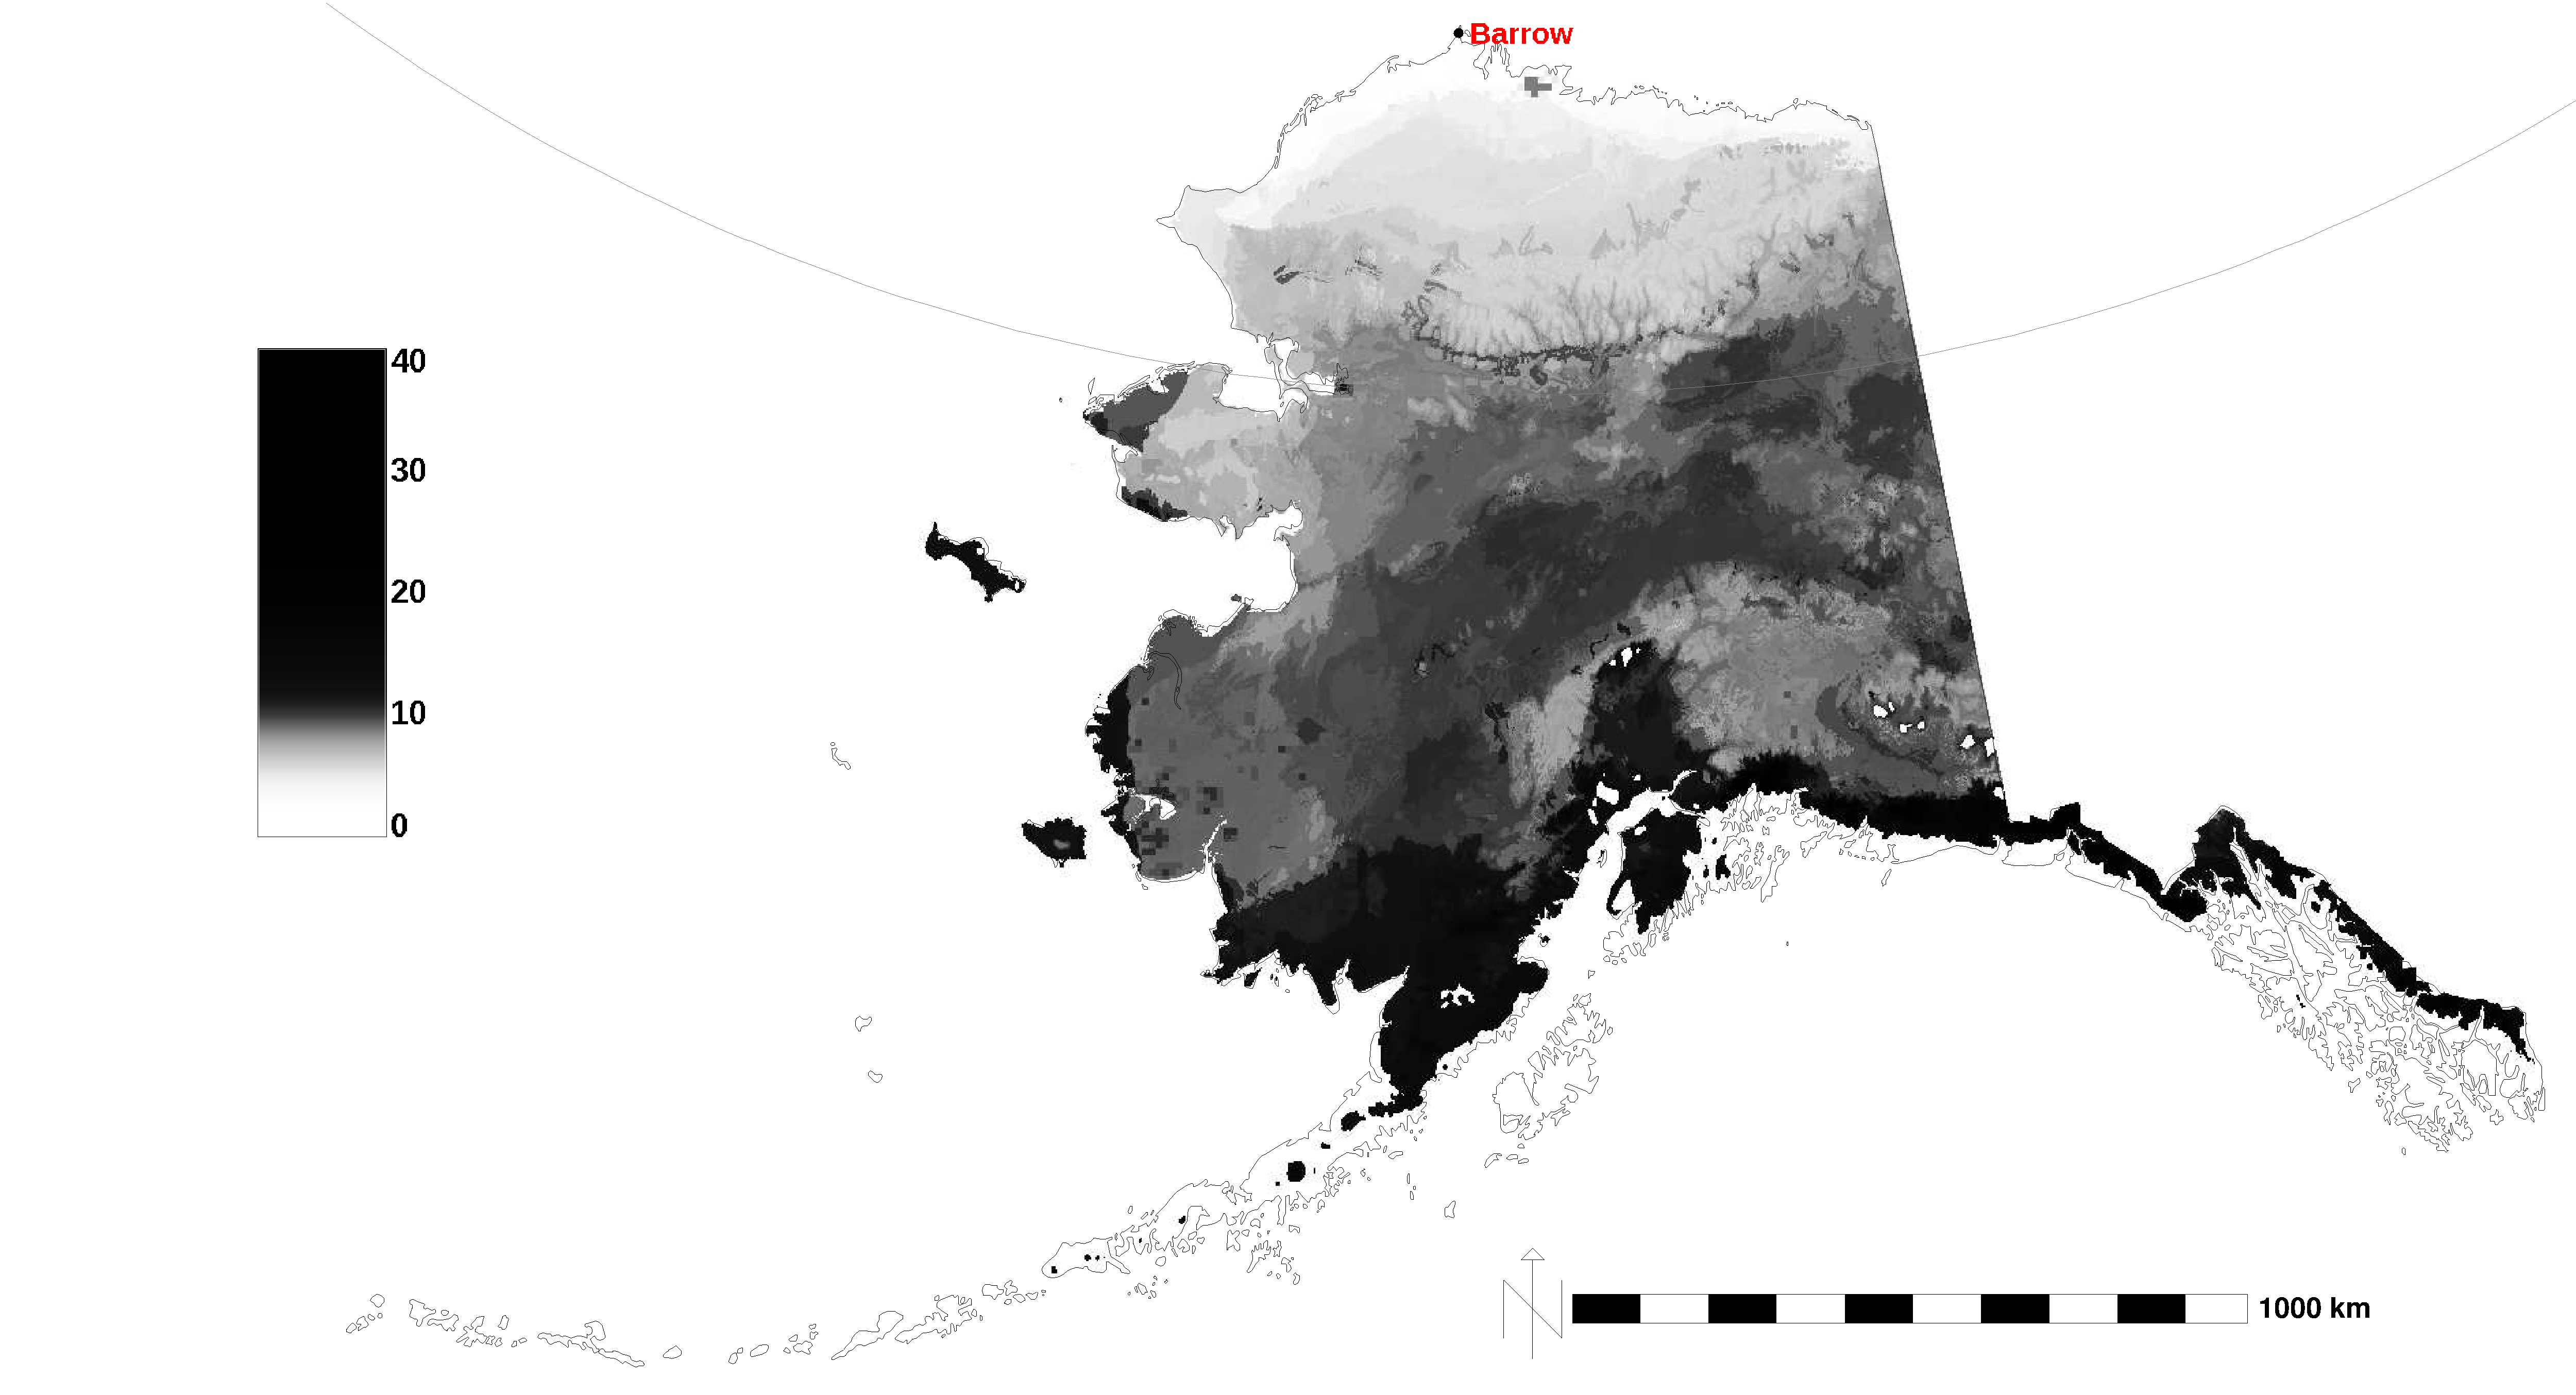
\includegraphics[width=0.50\textwidth]{ngee_figures/alaska_2090_2099_dem_Feb2012_k1000ness_1sites.pdf} \\
%   2000--2009 & 2090--2099 \\
%   \end{tabular}
%  %\caption{Cluster analysis.}
%  \label{fig:barrowness}
% \end{figure}
%
%As environmental conditions change, due primarily to increasing
%temperatures, climate gradients increase and the representativeness
%of Barrow will be diminished in the future.
%
%\end{frame}
%%%%%%%%%%%%%%%%%%%%%%%%%%%%%%%%%%%%%%%%%%%%%%%%%%%%%%%%%%%%%%%%%%%%%%%%%%%%
%
%%%%%%%%%%%%%%%%%%%%%%%%%%%%%%%%%%%%%%%%%%%%%%%%%%%%%%%%%%%%%%%%%%%%%%%%%%%%
%\begin{frame}
% \frametitle{Council and Prudhoe Bay Representativeness}
% \vskip-0.15in
% \setlength{\tabcolsep}{0pt}
% \begin{figure}
%   \begin{tabular}{cc}
%   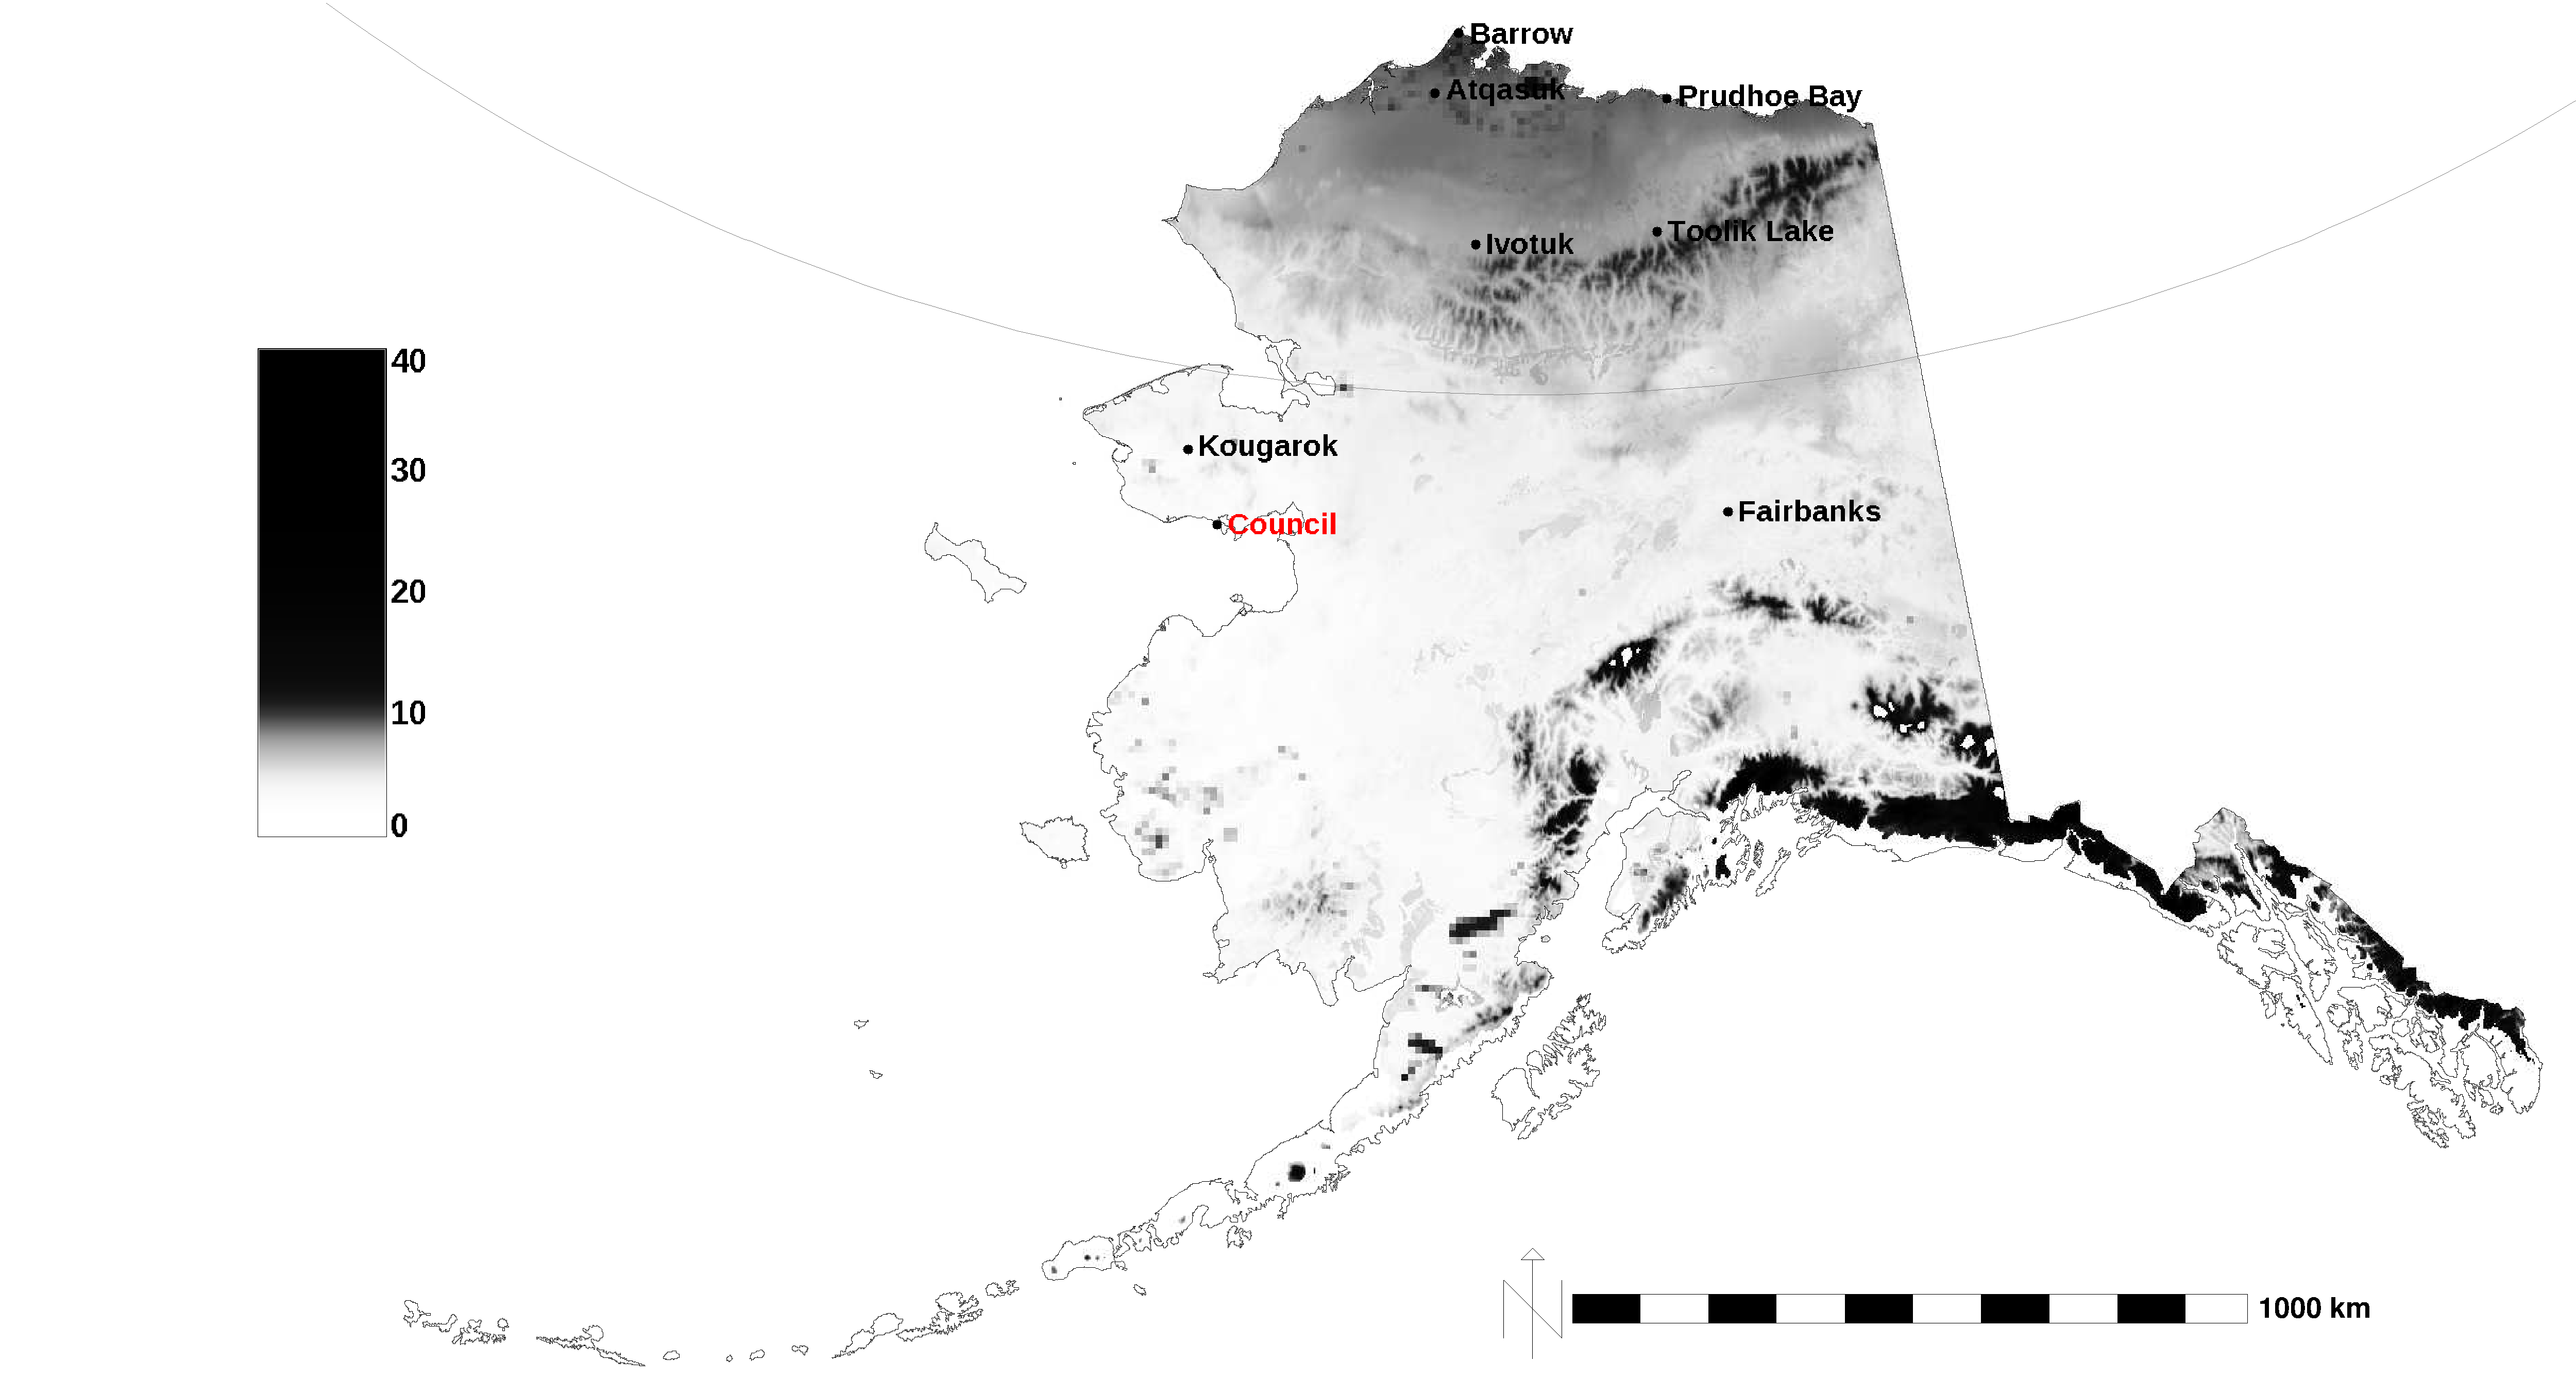
\includegraphics[width=0.50\textwidth]{ngee_figures/Councilness_2000_2009_on_2000_2009_point_global_dem_Feb2012.pdf} &
%   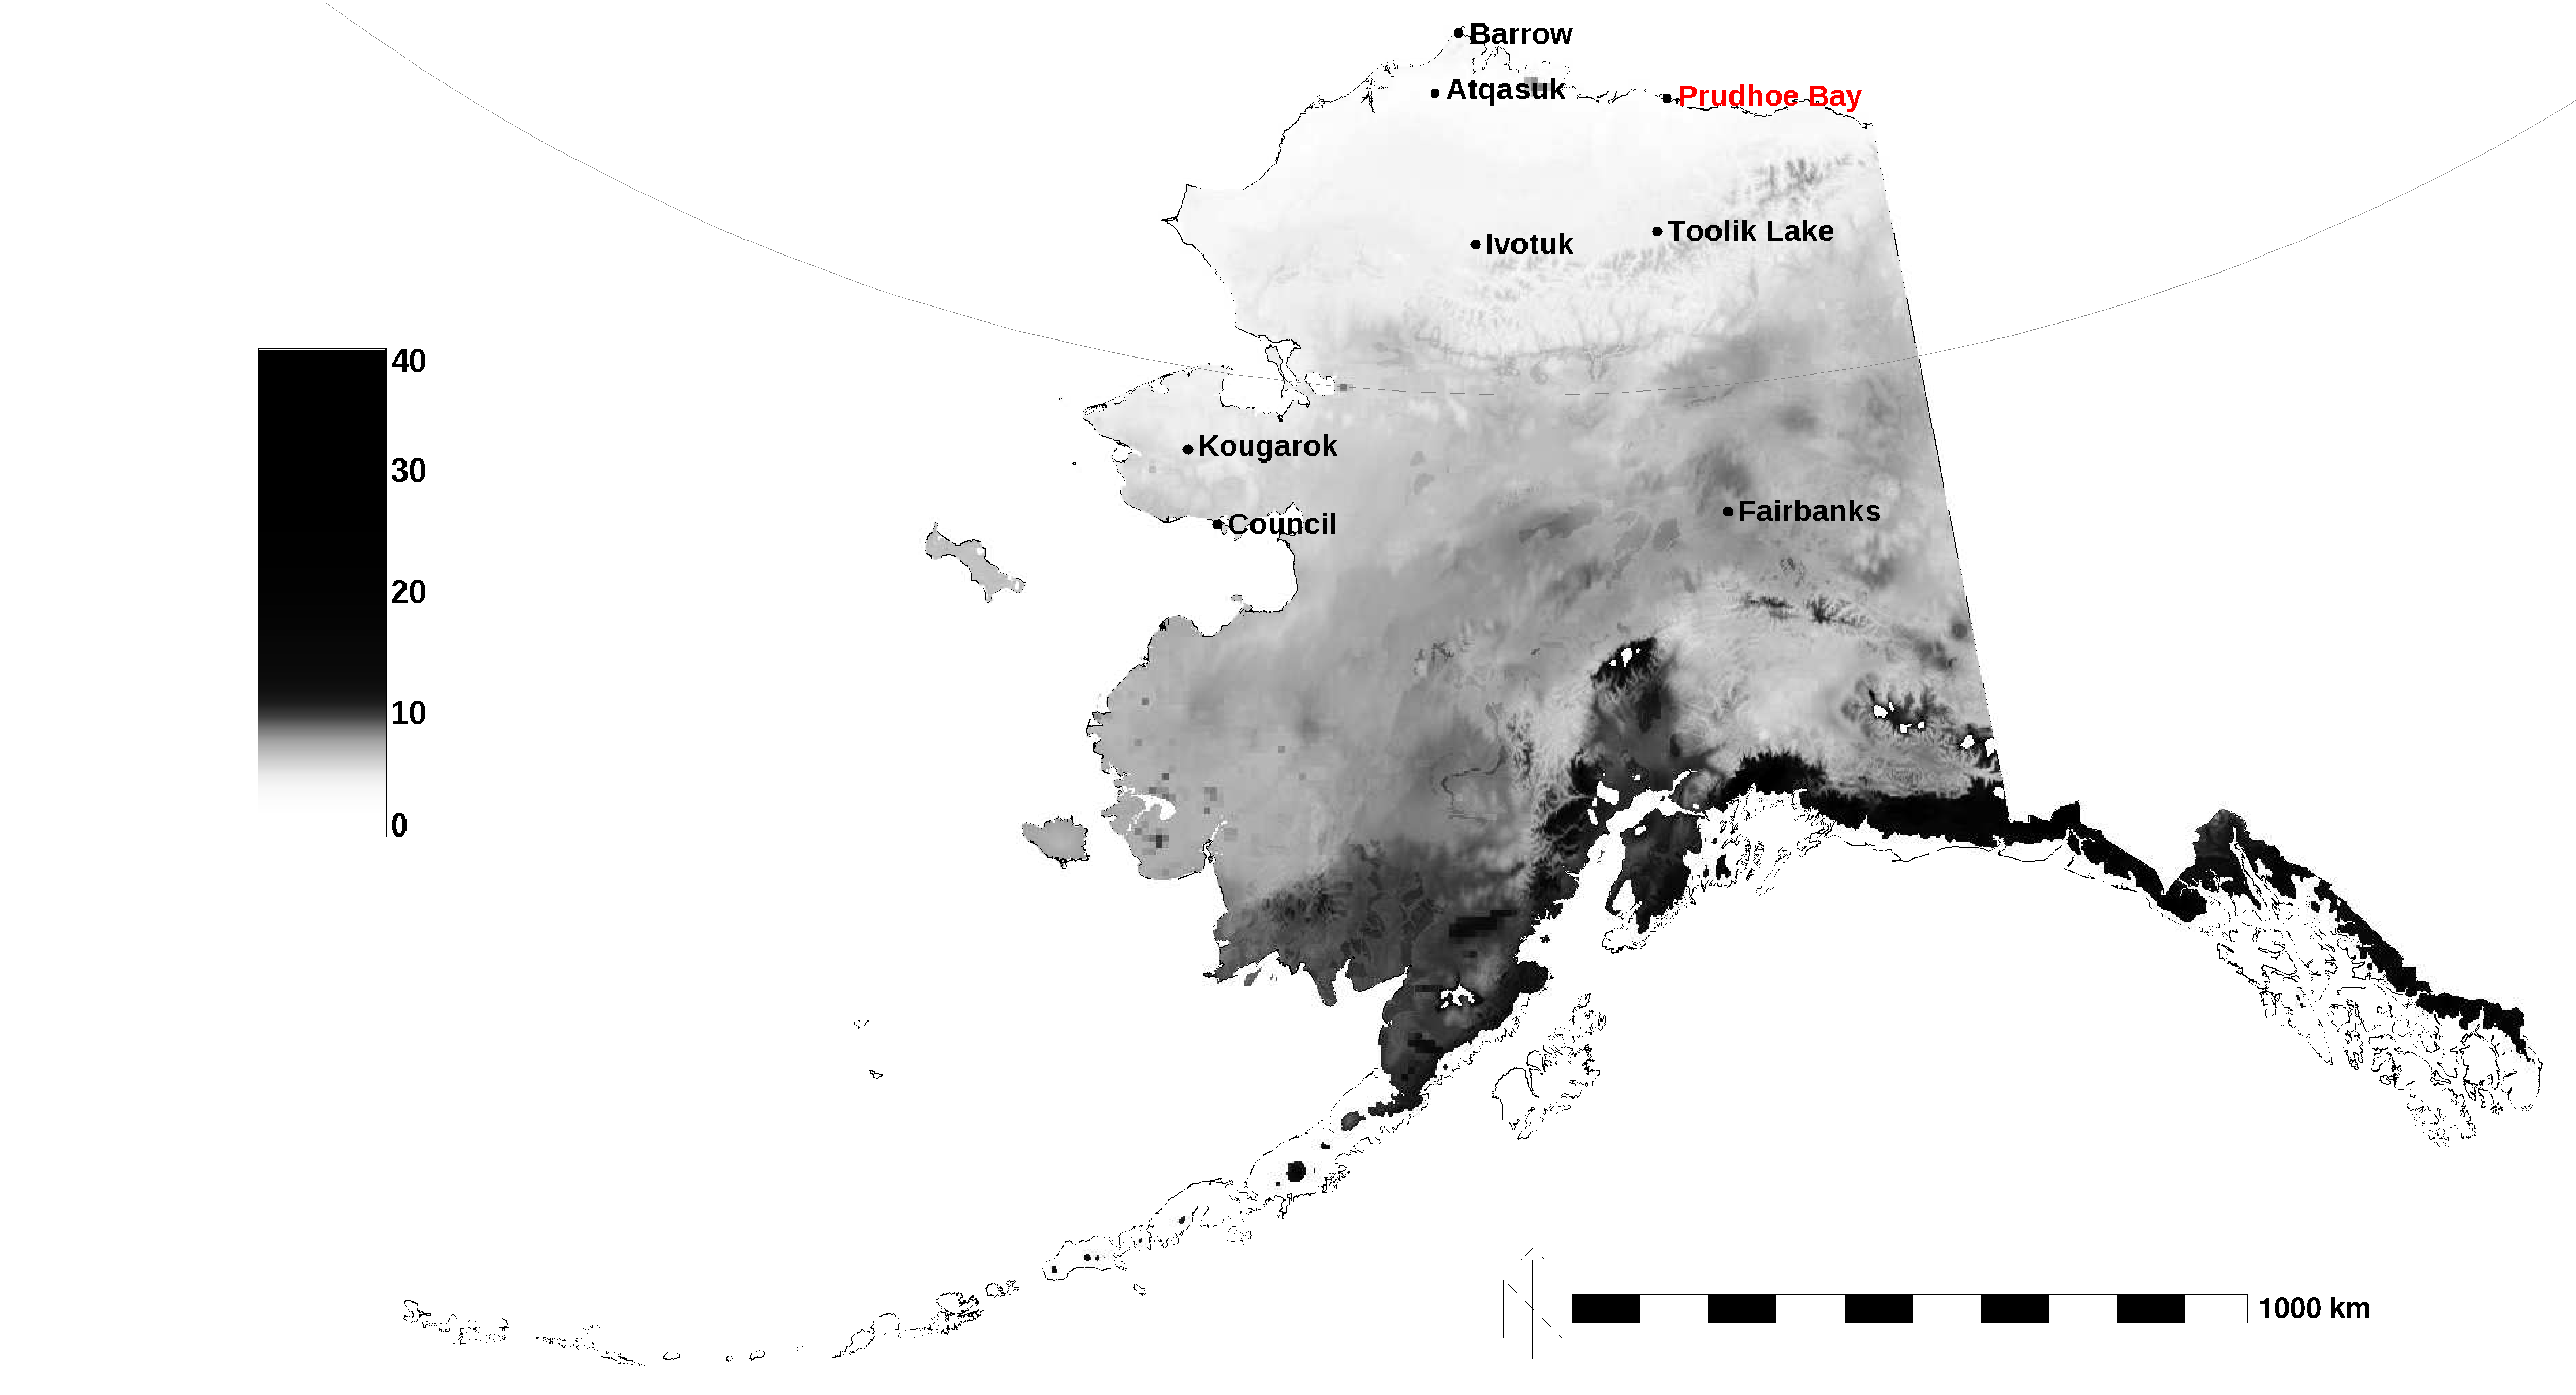
\includegraphics[width=0.50\textwidth]{ngee_figures/Prudhoe_bayness_2000_2009_on_2000_2009_point_global_dem_Feb2012.pdf} \\
%   Council & Prudhoe Bay \\
%   \end{tabular}
%  %\caption{Cluster analysis.}
%  \label{fig:council_and_prudhoe_bay}
% \end{figure}
%
%Representativeness analysis was performed for sites at Barrow, Council, Atqasuk,
%Ivotuk, Kougarok, Prudhoe Bay, Toolik Lake, and Fairbanks.
%
%\end{frame}
%%%%%%%%%%%%%%%%%%%%%%%%%%%%%%%%%%%%%%%%%%%%%%%%%%%%%%%%%%%%%%%%%%%%%%%%%%%%
%
%%%%%%%%%%%%%%%%%%%%%%%%%%%%%%%%%%%%%%%%%%%%%%%%%%%%%%%%%%%%%%%%%%%%%%%%%%%
\begin{frame}
 \frametitle{Network Representativeness: Barrow + Council}
 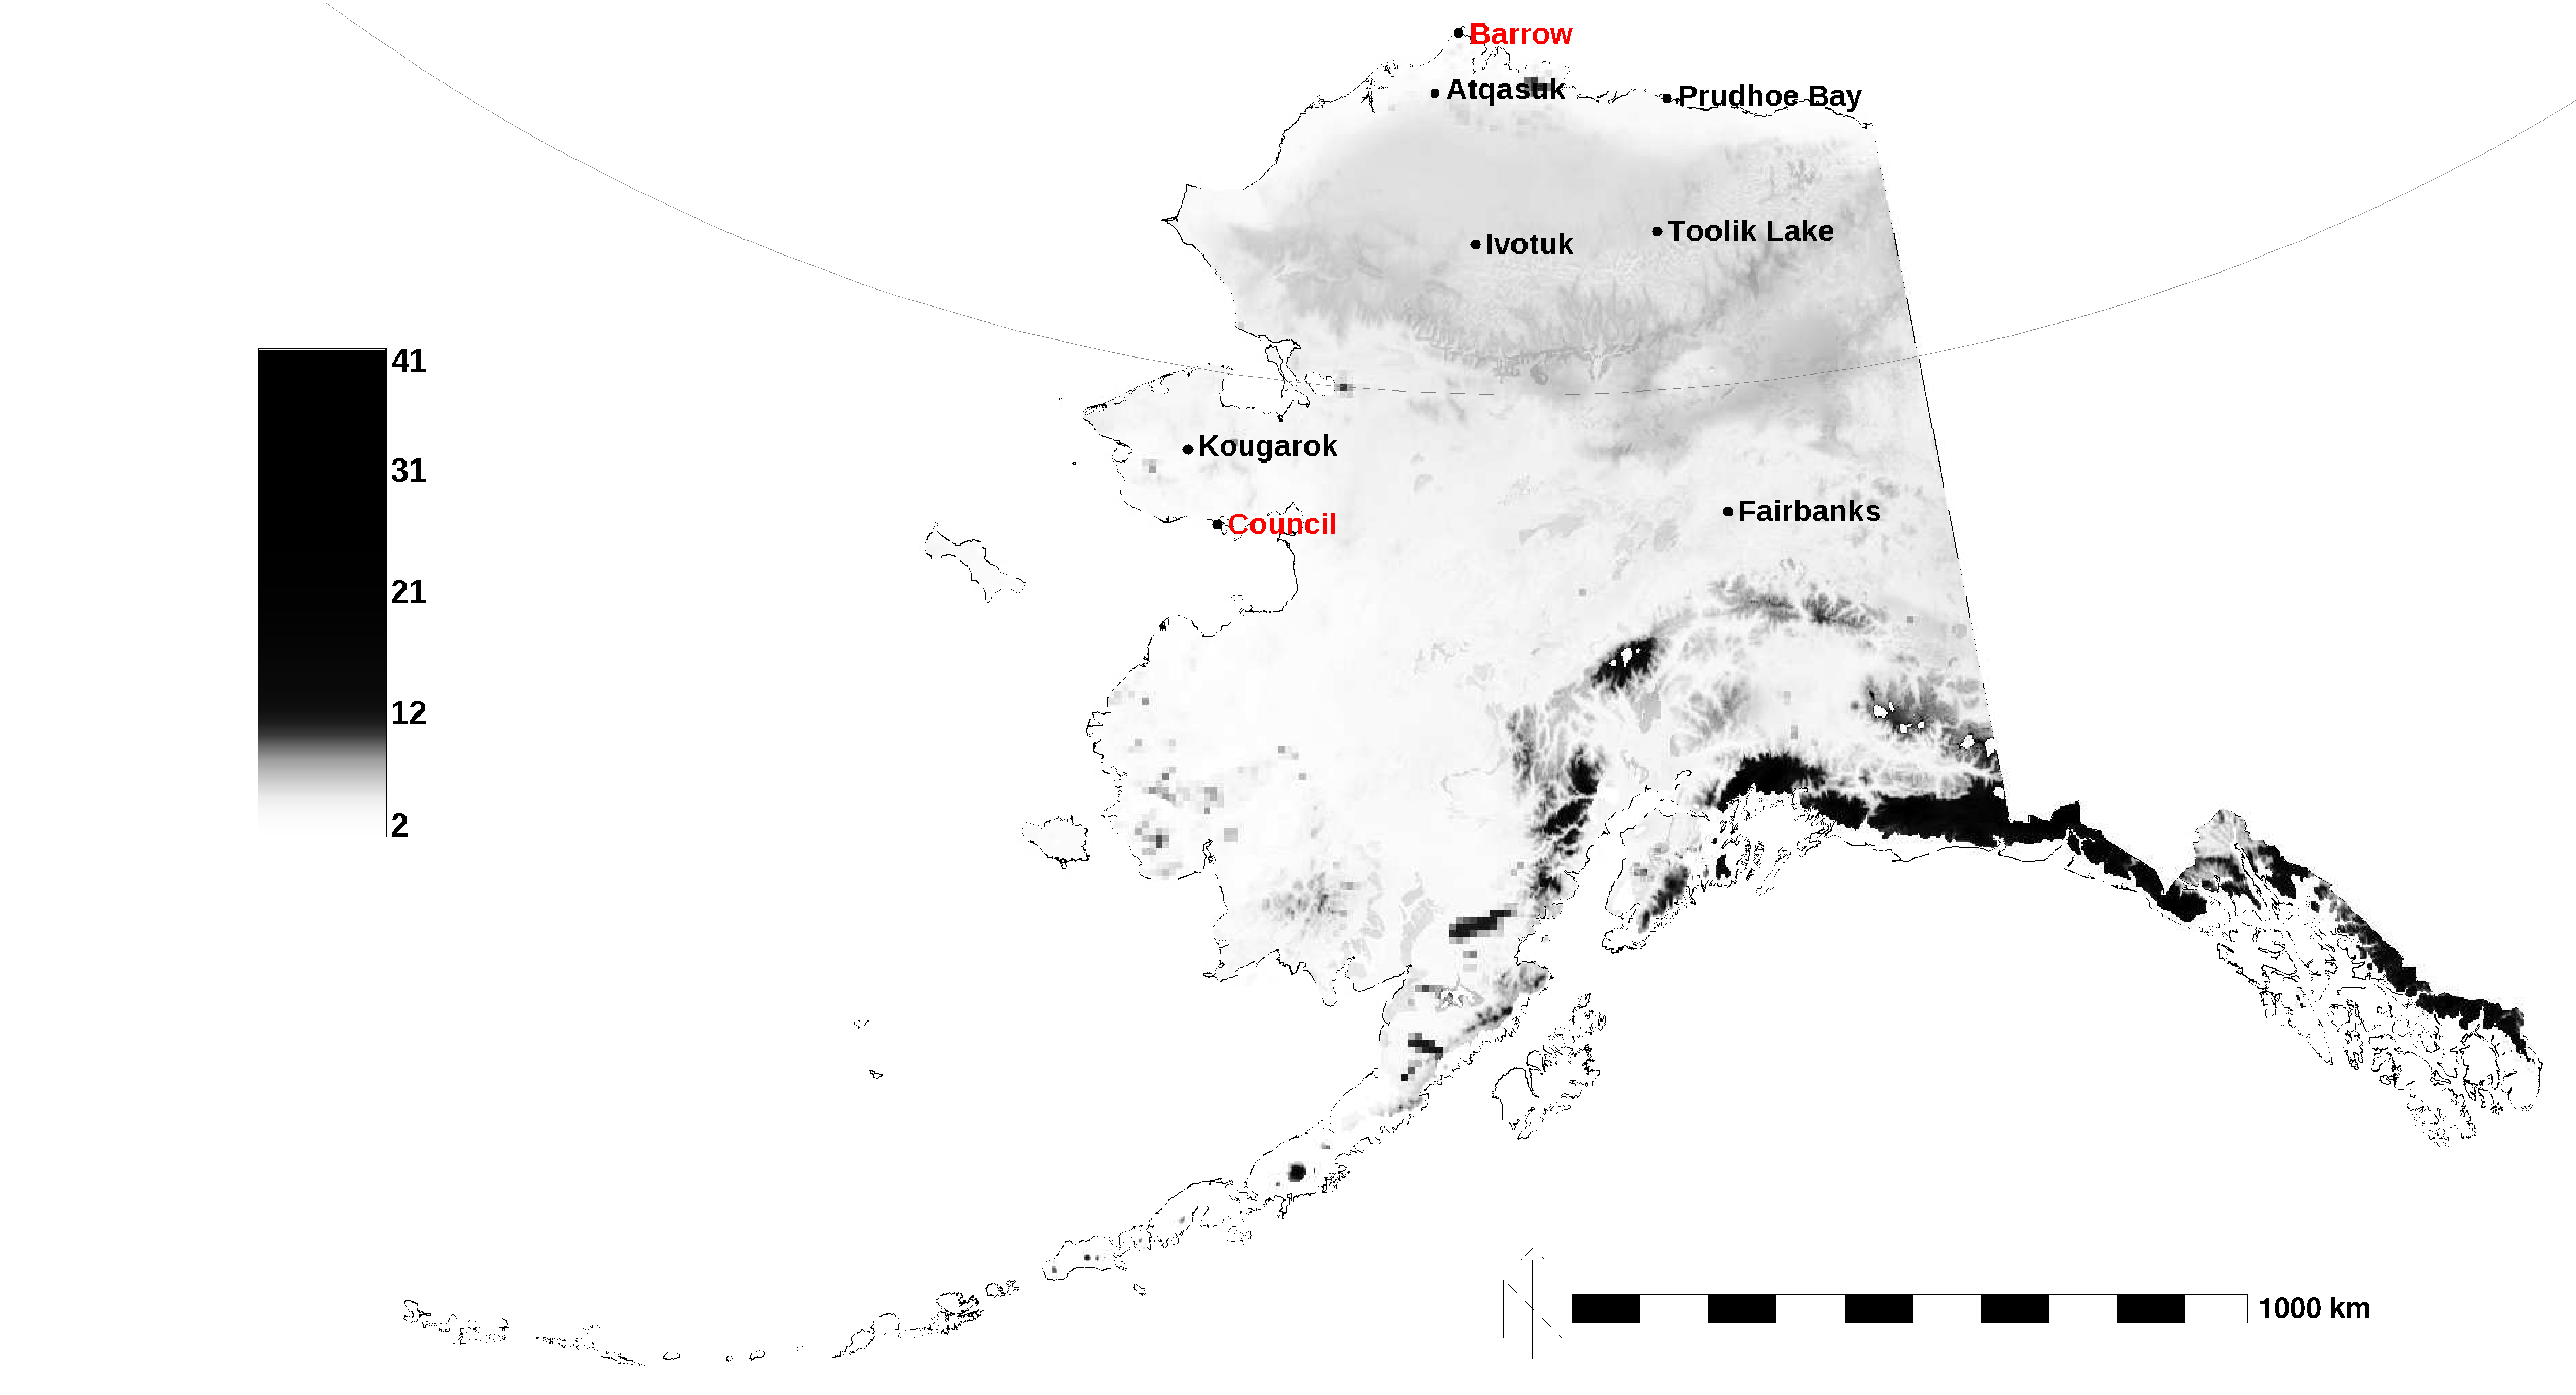
\includegraphics[width=\textwidth]{ngee_figures/Barrow-Councilness_2000-2009_on_2000-2009_point_global_dem_Feb2012_barscale.pdf} \\
  \vbox{\scriptsize\hfill\citep{Hoffman_LandscapeEcol_20131001}}

\medskip
Light-colored regions are well represented and dark-colored regions are
poorly represented by the sampling location listed in \textbf{\color{red}red}.
\end{frame}
%%%%%%%%%%%%%%%%%%%%%%%%%%%%%%%%%%%%%%%%%%%%%%%%%%%%%%%%%%%%%%%%%%%%%%%%%%%
%
%%%%%%%%%%%%%%%%%%%%%%%%%%%%%%%%%%%%%%%%%%%%%%%%%%%%%%%%%%%%%%%%%%%%%%%%%%%%
\begin{frame}
 \frametitle{Network Representativeness: All 8 Sites}
 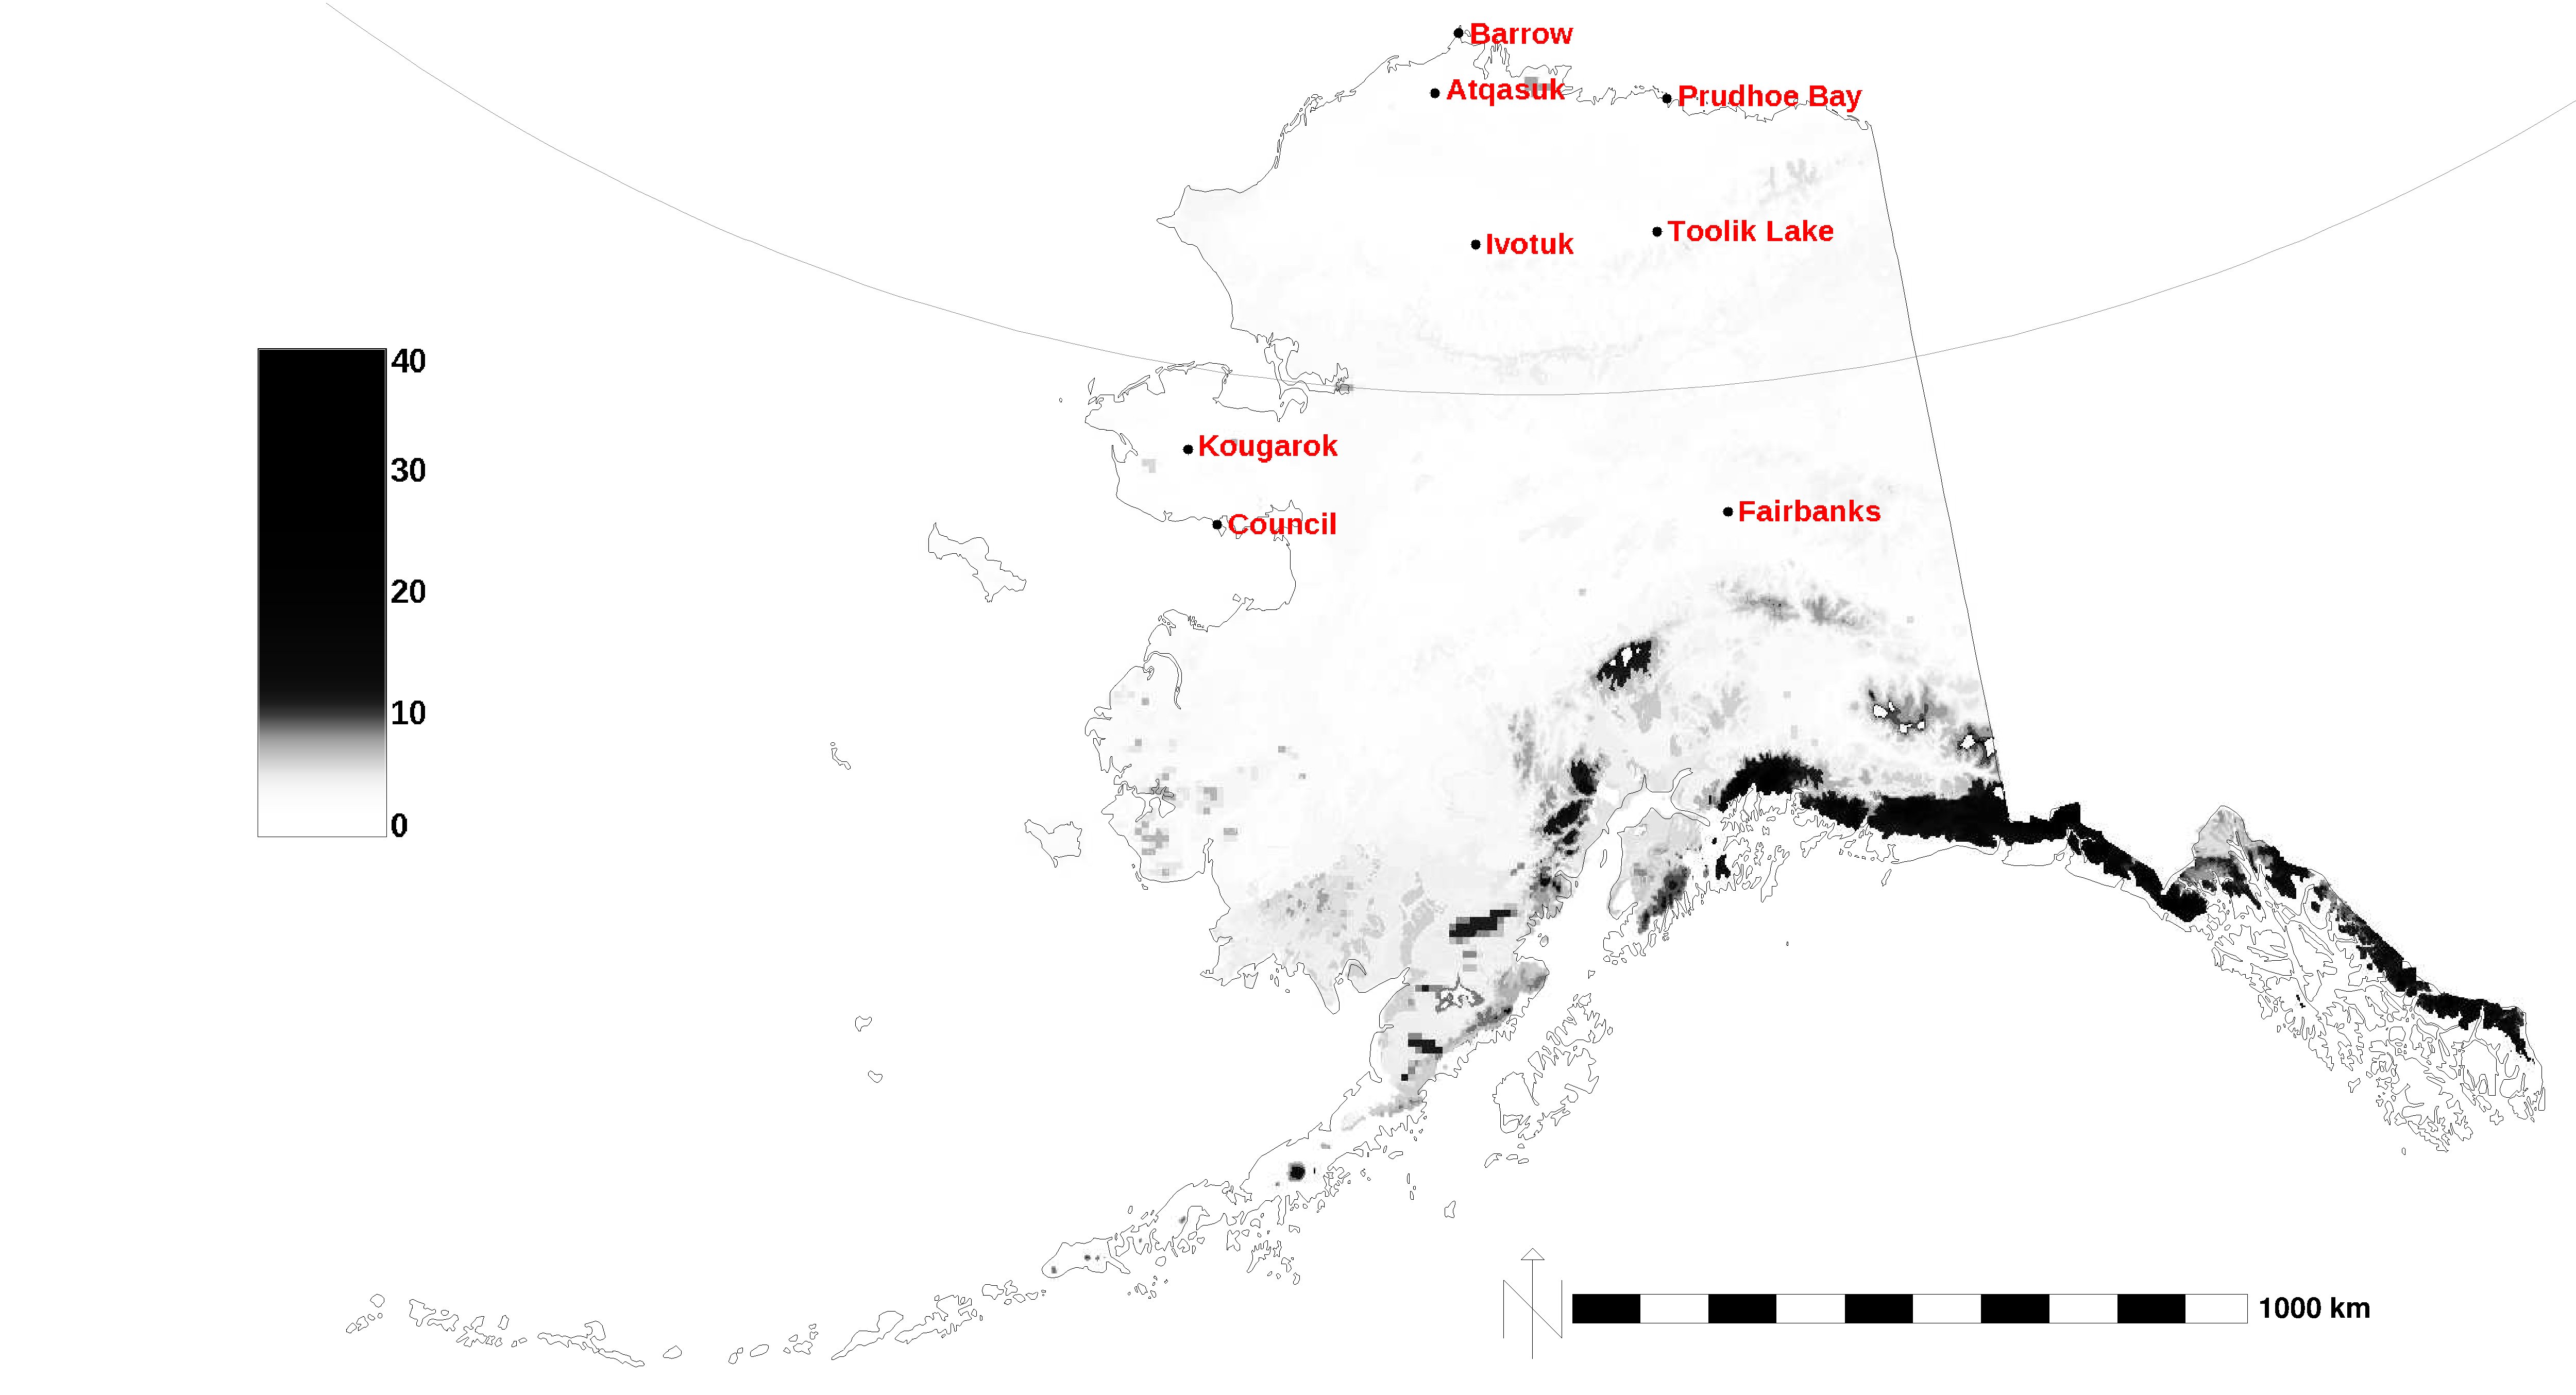
\includegraphics[width=\textwidth]{ngee_figures/alaska_2000_2009_dem_Feb2012_k1000ness_8sites.pdf} \\
  \vbox{\scriptsize\hfill\citep{Hoffman_LandscapeEcol_20131001}}

\medskip
Light-colored regions are well represented and dark-colored regions are
poorly represented by the sampling location listed in \textbf{\color{red}red}.
\end{frame}
%%%%%%%%%%%%%%%%%%%%%%%%%%%%%%%%%%%%%%%%%%%%%%%%%%%%%%%%%%%%%%%%%%%%%%%%%%%

%%%%%%%%%%%%%%%%%%%%%%%%%%%%%%%%%%%%%%%%%%%%%%%%%%%%%%%%%%%%%%%%%%%%%%%%%%%
% HoJo
%%%%%%%%%%%%%%%%%%%%%%%%%%%%%%%%%%%%%%%%%%%%%%%%%%%%%%%%%%%%%%%%%%%%%%%%%%%
\begin{frame}
 \frametitle{State Space Dissimilarities: 8 Sites, Present (2000--2009)}
 
\begin{table}
 \footnotesize\setlength{\tabcolsep}{2pt}
 \centering
  \caption{Site state space distances for the present (2000--2009) with DEM}
  \label{tbl:hojo_present}
  \begin{tabular}{r s s s s s s s}
   \toprule
   &  &  &  & \multicolumn{1}{c}{Toolik} &  & \multicolumn{1}{c}{Prudhoe} &  \\
   \multicolumn{1}{c}{\textbf{Sites}} & \multicolumn{1}{c}{Council} & \multicolumn{1}{c}{Atqasuk} & \multicolumn{1}{c}{Ivotuk} & \multicolumn{1}{c}{Lake} & \multicolumn{1}{c}{Kougarok} & \multicolumn{1}{c}{Bay} & \multicolumn{1}{c}{Fairbanks} \\
   \midrule
        Barrow &        9.13 &        4.53 &        5.90 &        5.87 &        7.98 &        3.57 &       12.16 \\
       Council &             &        8.69 &        6.37 &        7.00 &        2.28 &        8.15 &        5.05 \\
       Atqasuk &             &             &        5.18 &        5.23 &        7.79 &        1.74 &       10.66 \\
        Ivotuk &             &             &             &        1.81 &        5.83 &        4.48 &        7.90 \\
   Toolik Lake &             &             &             &             &        6.47 &        4.65 &        8.70 \\
      Kougarok &             &             &             &             &             &        7.25 &        5.57 \\
   Prudhoe Bay &             &             &             &             &             &             &       10.38 \\
   \bottomrule
  \end{tabular}
\end{table}


\end{frame}
%%%%%%%%%%%%%%%%%%%%%%%%%%%%%%%%%%%%%%%%%%%%%%%%%%%%%%%%%%%%%%%%%%%%%%%%%%%

%%%%%%%%%%%%%%%%%%%%%%%%%%%%%%%%%%%%%%%%%%%%%%%%%%%%%%%%%%%%%%%%%%%%%%%%%%%
\begin{frame}
 \frametitle{State Space Dissimilarities: 8 Sites, Future (2090--2099)}
 
\begin{table}
 \footnotesize\setlength{\tabcolsep}{2pt}
 \centering
  \caption{Site state space distances for the future (2090--2099) with DEM}
  \label{tbl:hojo_future}
  \begin{tabular}{r s s s s s s s}
   \toprule
   &  &  &  & \multicolumn{1}{c}{Toolik} &  & \multicolumn{1}{c}{Prudhoe} &  \\
   \multicolumn{1}{c}{\textbf{Sites}} & \multicolumn{1}{c}{Council} & \multicolumn{1}{c}{Atqasuk} & \multicolumn{1}{c}{Ivotuk} & \multicolumn{1}{c}{Lake} & \multicolumn{1}{c}{Kougarok} & \multicolumn{1}{c}{Bay} & \multicolumn{1}{c}{Fairbanks} \\
   \midrule
        Barrow &        8.87 &        4.89 &        6.88 &        6.94 &        8.04 &        4.18 &       11.95 \\
       Council &             &        8.82 &        6.93 &        7.74 &        2.43 &        8.24 &        5.66 \\
       Atqasuk &             &             &        5.86 &        5.84 &        8.15 &        2.30 &       10.16 \\
        Ivotuk &             &             &             &        2.01 &        7.27 &        4.75 &        7.51 \\
   Toolik Lake &             &             &             &             &        7.81 &        5.00 &        8.33 \\
      Kougarok &             &             &             &             &             &        7.89 &        6.42 \\
   Prudhoe Bay &             &             &             &             &             &             &        9.81 \\
   \bottomrule
  \end{tabular}
\end{table}


\end{frame}
%%%%%%%%%%%%%%%%%%%%%%%%%%%%%%%%%%%%%%%%%%%%%%%%%%%%%%%%%%%%%%%%%%%%%%%%%%%%

%%%%%%%%%%%%%%%%%%%%%%%%%%%%%%%%%%%%%%%%%%%%%%%%%%%%%%%%%%%%%%%%%%%%%%%%%%%
\begin{frame}
 \frametitle{State Space Dissimilarities: 8 Sites, Present and Future}
 
\begin{table}
 \scriptsize\setlength{\tabcolsep}{1pt}
 \centering
  \caption{Site state space distances between the present (2000--2009) and the future (2090--2099) with DEM}
  \label{tbl:hojo_present_future}
  \begin{tabular}{c r s s s s s s s s}
   \toprule
    &  & \multicolumn{8}{c}{\textit{Future (2090--2099)}} \\
    & &  &  &  &  & \multicolumn{1}{c}{Toolik} &  & \multicolumn{1}{c}{Prudhoe} &  \\
    & \multicolumn{1}{c}{\textbf{Sites}} & \multicolumn{1}{c}{Barrow} & \multicolumn{1}{c}{Council} & \multicolumn{1}{c}{Atqasuk} & \multicolumn{1}{c}{Ivotuk} & \multicolumn{1}{c}{Lake} & \multicolumn{1}{c}{Kougarok} & \multicolumn{1}{c}{Bay} & \multicolumn{1}{c}{Fairbanks} \\
   \midrule
   \multirow{8}{*}{\begin{sideways}\textit{Present (2000--2009)}\end{sideways}}
    &      Barrow &        3.31 &        9.67 &        4.63 &        6.05 &        5.75 &        9.02 &        3.69 &       11.67 \\
    &     Council &        8.38 &        1.65 &        8.10 &        5.91 &        6.87 &        3.10 &        7.45 &        5.38 \\
    &     Atqasuk &        6.01 &        9.33 &        2.42 &        5.46 &        5.26 &        8.97 &        2.63 &       10.13 \\
    &      Ivotuk &        7.06 &        7.17 &        5.83 &        1.53 &        2.05 &        7.25 &        4.87 &        7.40 \\
    & Toolik Lake &        7.19 &        7.67 &        6.07 &        2.48 &        1.25 &        7.70 &        5.23 &        8.16 \\
    &    Kougarok &        7.29 &        3.05 &        6.92 &        5.57 &        6.31 &        2.51 &        6.54 &        5.75 \\
    & Prudhoe Bay &        5.29 &        8.80 &        3.07 &        4.75 &        4.69 &        8.48 &        1.94 &        9.81 \\
    &   Fairbanks &       12.02 &        5.49 &       10.36 &        7.83 &        8.74 &        6.24 &       10.10 &        1.96 \\
   \bottomrule
  \end{tabular}
\end{table}


\end{frame}
%%%%%%%%%%%%%%%%%%%%%%%%%%%%%%%%%%%%%%%%%%%%%%%%%%%%%%%%%%%%%%%%%%%%%%%%%%%%

%%%%%%%%%%%%%%%%%%%%%%%%%%%%%%%%%%%%%%%%%%%%%%%%%%%%%%%%%%%%%%%%%%%%%%%%%%%
\begin{frame}{Representativeness: A Quantitative Approach for Scaling}
 \begin{itemize}
  \item MSTC provides a quantitative framework for stratifying sampling domains, informing site selection, and determining representativeness of measurements.
  \item Representativeness analysis provides a systematic approach for up-scaling point measurements to larger domains.
  \item Methodology is independent of resolution, thus can be applied from site/plot scale to landscape/climate scale.
  \item It can be extended to include finer spatiotemporal scales, more geophysical characteristics, and remote sensing data.
  \item Methodology described in Open Access paper: \\
  \textrm{\small Hoffman, F. M., J. Kumar, R. T. Mills, and W. W. Hargrove (2013), ``Representativeness-Based Sampling Network Design for the State of Alaska.'' \textit{Landscape Ecol.}, 28(8):1567--1586. doi:\href{http://dx.doi.org/10.1007/s10980-013-9902-0}{10.1007/s10980-013-9902-0}.}
  \nocite{Hoffman_LandscapeEcol_20131001}
  \item Resulting maps and data available from (the first NGEE Arctic Data DOI): \textrm{\small doi:\href{http://dx.doi.org/10.5440/1108686}{10.5440/1108686}}.
 \end{itemize}

\end{frame}
%%%%%%%%%%%%%%%%%%%%%%%%%%%%%%%%%%%%%%%%%%%%%%%%%%%%%%%%%%%%%%%%%%%%%%%%%%

\subsection[Barrow]{Barrow Environmental Observatory Representativeness}
%\section{BEO Representativeness}
%%%%%%%%%%%%%%%%%%%%%%%%%%%%%%%%%%%%%%%%%%%%%%%%%%%%%%%%%%%%%%%%%%%%%%%%%%%%%%%
\begin{frame}
 \frametitle{Barrow Environmental Observatory (BEO)}
 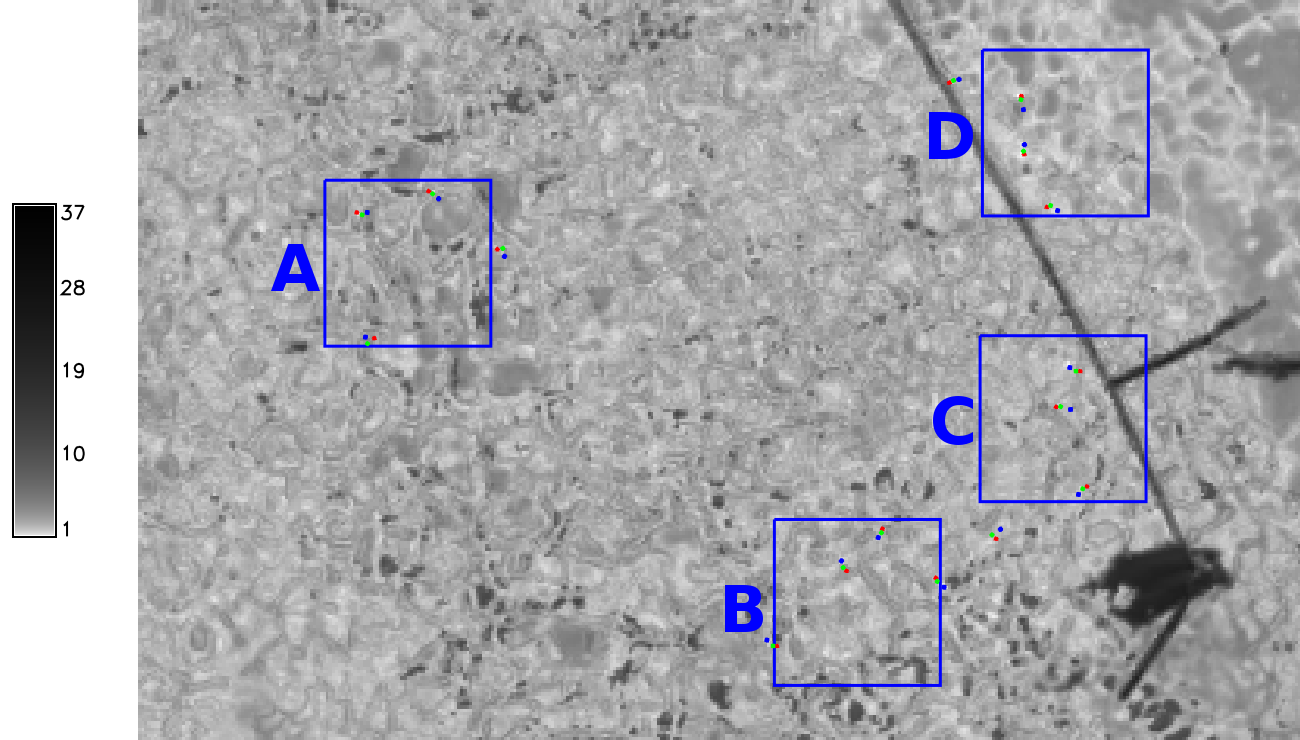
\includegraphics[width=0.47\textwidth]{beo_figures/ABCDv2.png}
 \hfill
 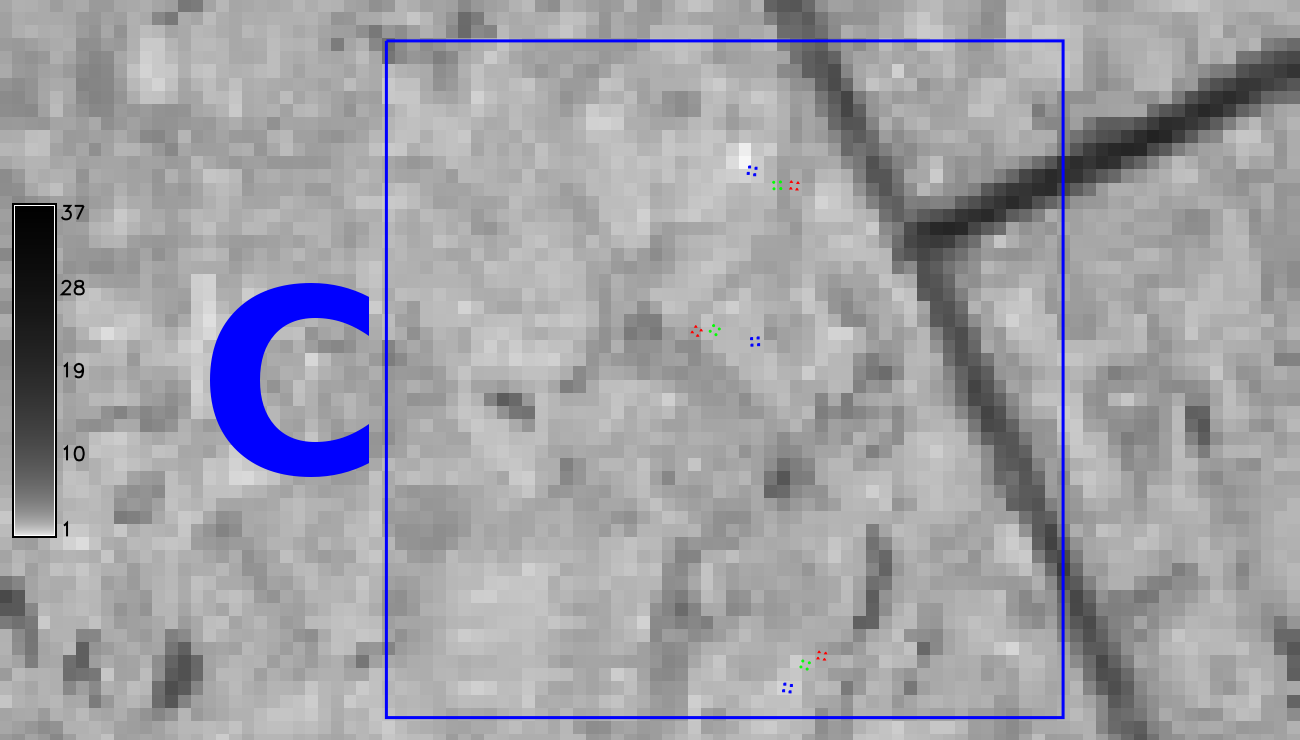
\includegraphics[width=0.47\textwidth]{beo_figures/Cv2.png} \\
 \vbox{\scriptsize\hfill (Kumar et al., in prep)}

\medskip
Representativeness map for vegetation sampling points for A, B, C, and D
sampling area (left) and zoomed in on the C samping area (right) developed
from WorldView2 satellite images for the year 2010 and LiDAR data.

\medskip
Vegetation sampling locations represent polygon troughs (red), edges
(green), and centers (blue).

\end{frame}
%%%%%%%%%%%%%%%%%%%%%%%%%%%%%%%%%%%%%%%%%%%%%%%%%%%%%%%%%%%%%%%%%%%%%%%%%%%%%%%

%%%%%%%%%%%%%%%%%%%%%%%%%%%%%%%%%%%%%%%%%%%%%%%%%%%%%%%%%%%%%%%%%%%%%%%%%%%%%%%
\begin{frame}

\vskip-0.15in
\begin{figure}
 {\centering\footnotesize
 \hfil
 \subfigure[dry tundra gramanoid]{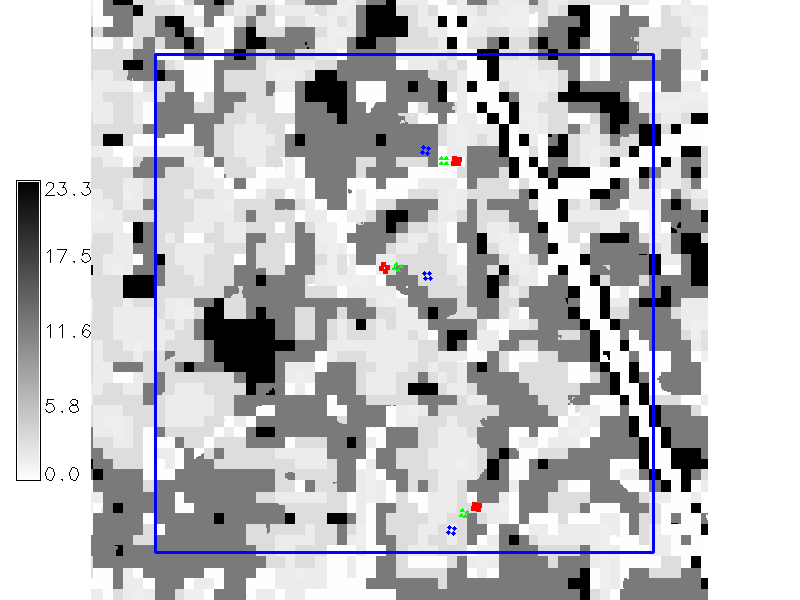
\includegraphics[width=0.40\textwidth]{beo_figures/areac_dry_tundra_graminoid.png}\label{fig:areac_dry_tundra_graminoid}}
 \hfil
 \subfigure[forb]{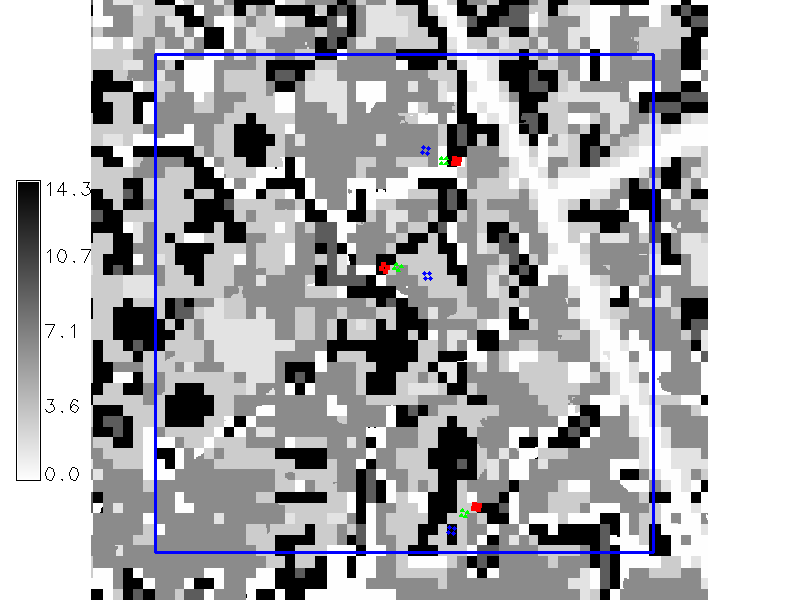
\includegraphics[width=0.40\textwidth]{beo_figures/areac_forb.png}\label{fig:areac_forb}}
 \hfil \\
 \hfil
 \subfigure[lichen]{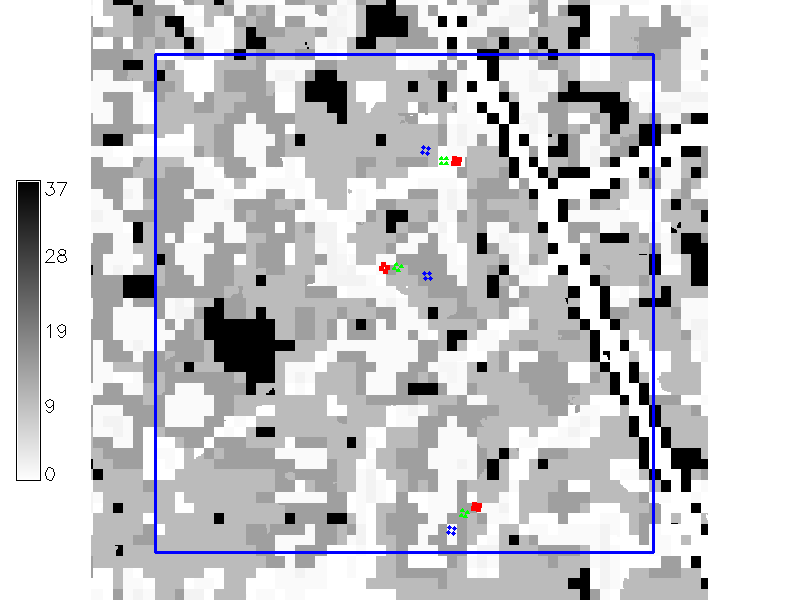
\includegraphics[width=0.40\textwidth]{beo_figures/areac_lichen.png}\label{fig:areac_lichen}}
 \hfil
 \subfigure[moss]{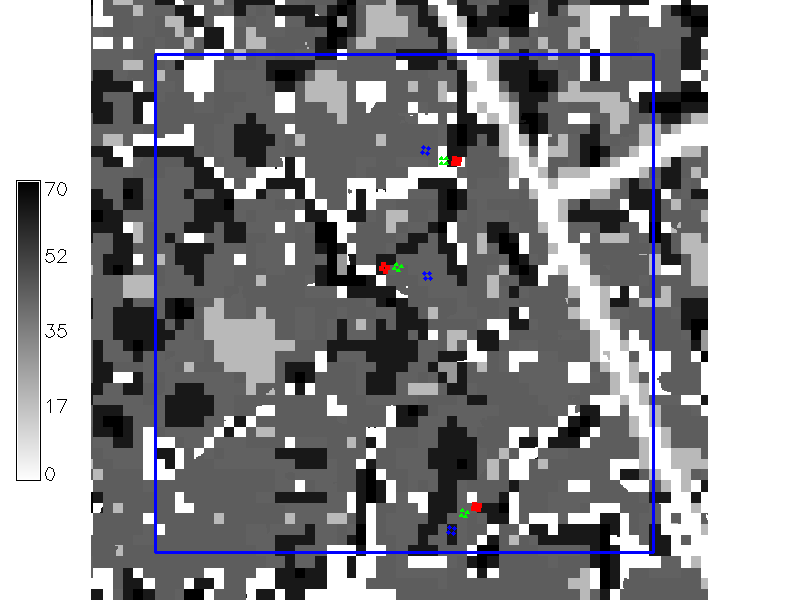
\includegraphics[width=0.40\textwidth]{beo_figures/areac_moss.png}\label{fig:areac_moss}}
 \hfil \\
 \vskip-0.10in\vbox{\scriptsize\hfill (Kumar et al., in prep)}
 }
% \caption{Using WorldView2 satellite imagery and LiDAR data, plant
% functional type (PFT) distributions were scaled up to each sampling
% area based on their proportion at vegetation sampling locations.
% Four such PFT distribution maps are shown for area C.}
 \label{fig:areac_pfts}
\end{figure}

\vskip-0.15in
Example plant functional type (PFT) distributions scaled up from vegetation sampling locations.

\end{frame}
%%%%%%%%%%%%%%%%%%%%%%%%%%%%%%%%%%%%%%%%%%%%%%%%%%%%%%%%%%%%%%%%%%%%%%%%%%%%%%%

\subsection[NGEE Tropics]{NGEE Tropics Representativeness}
%%%%%%%%%%%%%%%%%%%%%%%%%%%%%%%%%%%%%%%%%%%%%%%%%%%%%%%%%%%%%%%%%%%%%%%%%%%%%%%
\begin{frame}
 \begin{center}
  \vbox{\Huge\color{CCSIGreen}\textbf{An Approach for Selecting Distributed Sampling Sites for NGEE Tropics}}
 \end{center}
\end{frame}
%%%%%%%%%%%%%%%%%%%%%%%%%%%%%%%%%%%%%%%%%%%%%%%%%%%%%%%%%%%%%%%%%%%%%%%%%%%%%%%
%%%%%%%%%%%%%%%%%%%%%%%%%%%%%%%%%%%%%%%%%%%%%%%%%%%%%%%%%%%%%%%%%%%%%%%%%%%%%%%
%{ % Approach for prioritizing field activities and selecting sites
%\usebackgroundtemplate{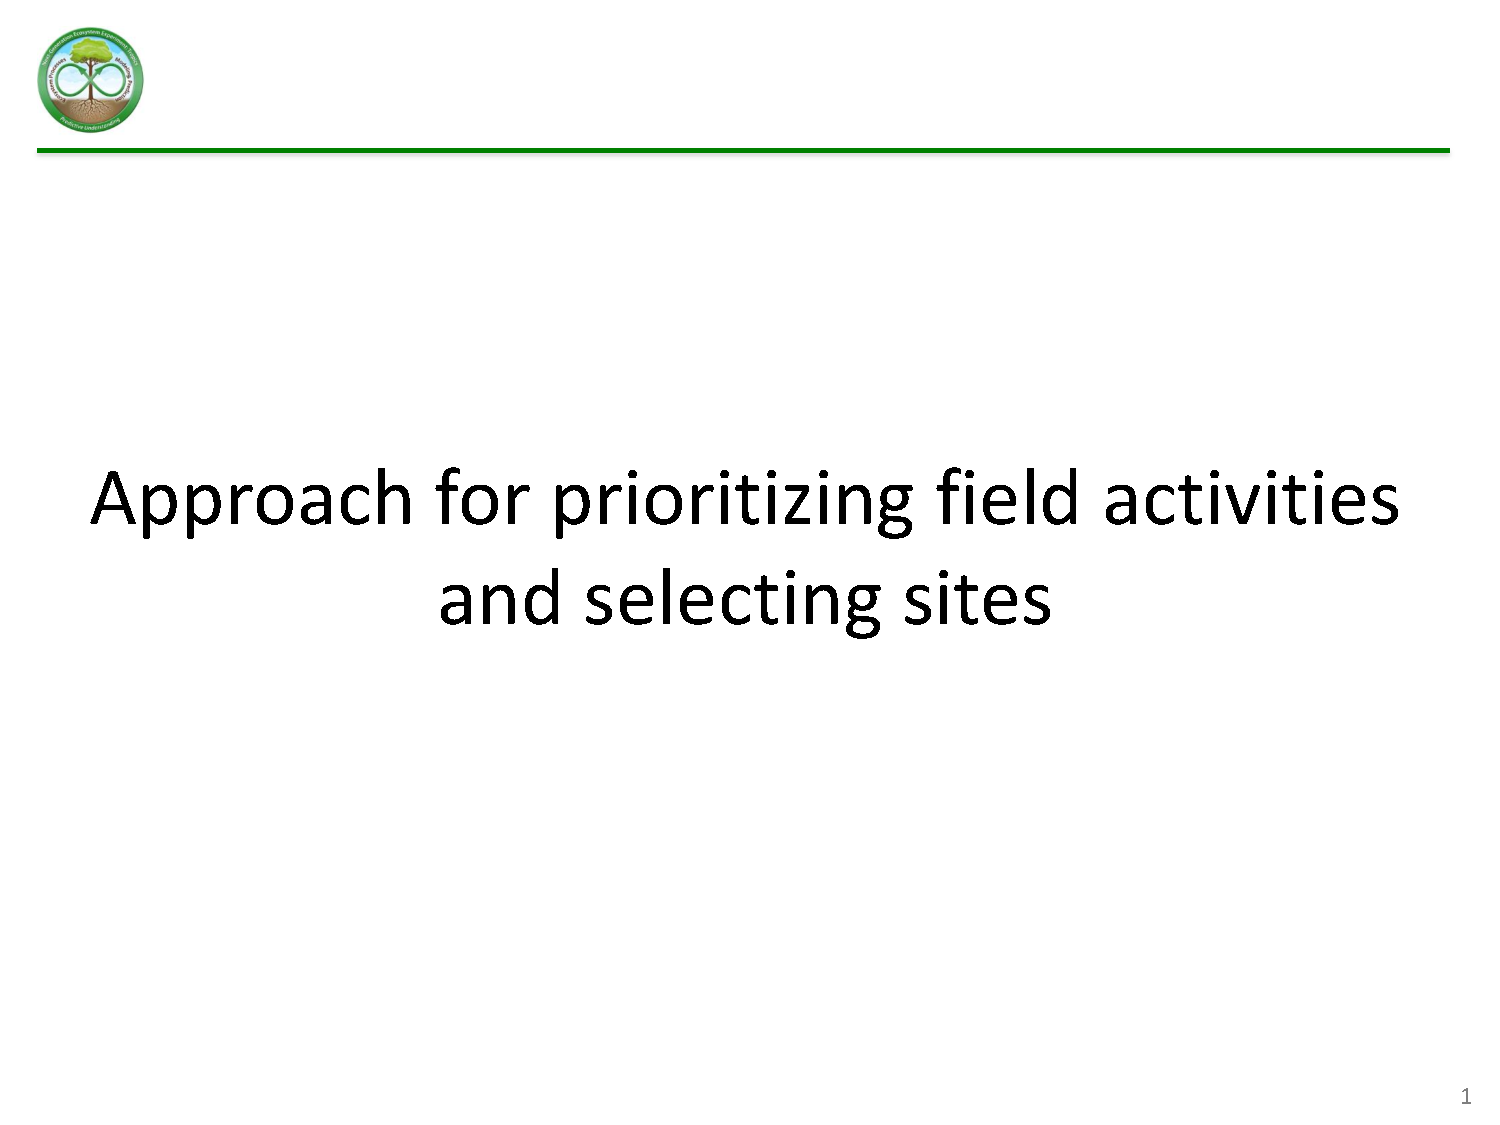
\includegraphics[width=\paperwidth,page=1]{NGEE_Tropics_Field_Activities_Detail_20140529v3.pdf}}
%\begin{frame}
%\end{frame}
%}
%%%%%%%%%%%%%%%%%%%%%%%%%%%%%%%%%%%%%%%%%%%%%%%%%%%%%%%%%%%%%%%%%%%%%%%%%%%%%%%

%%%%%%%%%%%%%%%%%%%%%%%%%%%%%%%%%%%%%%%%%%%%%%%%%%%%%%%%%%%%%%%%%%%%%%%%%%%%%%%
%{ % Process for Prioritizing Field Activities
%\usebackgroundtemplate{\includegraphics[width=\paperwidth,page=2]{NGEE_Tropics_Field_Activities_Detail_20140529v3.pdf}}
%\begin{frame}
%\end{frame}
%}
%%%%%%%%%%%%%%%%%%%%%%%%%%%%%%%%%%%%%%%%%%%%%%%%%%%%%%%%%%%%%%%%%%%%%%%%%%%%%%%
%%%%%%%%%%%%%%%%%%%%%%%%%%%%%%%%%%%%%%%%%%%%%%%%%%%%%%%%%%%%%%%%%%%%%%%%%%%%%%%
%{ % Quantify model uncertaintity contributions from parameters, modules
%\usebackgroundtemplate{\includegraphics[width=\paperwidth,page=3]{NGEE_Tropics_Field_Activities_Detail_20140529v3.pdf}}
%\begin{frame}
%\end{frame}
%}
%%%%%%%%%%%%%%%%%%%%%%%%%%%%%%%%%%%%%%%%%%%%%%%%%%%%%%%%%%%%%%%%%%%%%%%%%%%%%%%
%%%%%%%%%%%%%%%%%%%%%%%%%%%%%%%%%%%%%%%%%%%%%%%%%%%%%%%%%%%%%%%%%%%%%%%%%%%%%%%
%{ % Rank processes by contribution to model variance
%\usebackgroundtemplate{\includegraphics[width=\paperwidth,page=4]{NGEE_Tropics_Field_Activities_Detail_20140529v3.pdf}}
%\begin{frame}
%\end{frame}
%}
%%%%%%%%%%%%%%%%%%%%%%%%%%%%%%%%%%%%%%%%%%%%%%%%%%%%%%%%%%%%%%%%%%%%%%%%%%%%%%%
%%%%%%%%%%%%%%%%%%%%%%%%%%%%%%%%%%%%%%%%%%%%%%%%%%%%%%%%%%%%%%%%%%%%%%%%%%%%%%%
%{ % Alaska Ecoregions and Representativeness
%\usebackgroundtemplate{\includegraphics[width=\paperwidth,page=5]{NGEE_Tropics_Field_Activities_Detail_20140529v3.pdf}}
%\begin{frame}
%\end{frame}
%}
%%%%%%%%%%%%%%%%%%%%%%%%%%%%%%%%%%%%%%%%%%%%%%%%%%%%%%%%%%%%%%%%%%%%%%%%%%%%%%%
%%%%%%%%%%%%%%%%%%%%%%%%%%%%%%%%%%%%%%%%%%%%%%%%%%%%%%%%%%%%%%%%%%%%%%%%%%%%%%%
{ % ForestGEO Network Global Representativeness
\usebackgroundtemplate{\includegraphics[width=\paperwidth,page=6]{NGEE_Tropics_Field_Activities_Detail_20140529v3.pdf}}
\begin{frame}
\end{frame}
}
%%%%%%%%%%%%%%%%%%%%%%%%%%%%%%%%%%%%%%%%%%%%%%%%%%%%%%%%%%%%%%%%%%%%%%%%%%%%%%%
%\section{Forest Representativeness}
%%%%%%%%%%%%%%%%%%%%%%%%%%%%%%%%%%%%%%%%%%%%%%%%%%%%%%%%%%%%%%%%%%%%%%%%%%%%%%%%
%\begin{frame}
% \frametitle{ForestGEO Network Global Representativeness}
% \includegraphics[width=\textwidth]{forest_figures/forestGEOall_years_2013.png} \\
% \vskip-0.25in\vbox{\scriptsize\hfill (Maddalena et al., in prep)}
%
%\smallskip
%Light-colored regions are well represented and dark-colored regions are
%poorly represented by the ForestGEO sampling network.
%
%\smallskip
%Animation of the time evolution of the ForestGEO network: \href{https://climate.ornl.gov/~jkumar/share/forestGEOall_years.gif}{https://climate.ornl.gov/$\sim$jkumar/share/forestGEOall\_years.gif}
%
%\end{frame}
%%%%%%%%%%%%%%%%%%%%%%%%%%%%%%%%%%%%%%%%%%%%%%%%%%%%%%%%%%%%%%%%%%%%%%%%%%%%%%%%

%%%%%%%%%%%%%%%%%%%%%%%%%%%%%%%%%%%%%%%%%%%%%%%%%%%%%%%%%%%%%%%%%%%%%%%%%%%%%%%
\begin{frame}
 \frametitle{Triple-Network Global Representativeness}
 \includegraphics[width=\textwidth]{forest_figures/allNetworks_global_RGB_histEq_wheelLegend.png} \\
 \vskip-0.25in\vbox{\scriptsize\hfill (Maddalena et al., in prep)}

\medskip
Map indicates which sampling network offers the most representative
coverage at any location. Every location is made up of a combination of
three primary colors from Fluxnet (red), ForestGEO (green), and RAINFOR
(blue).

\end{frame}
%%%%%%%%%%%%%%%%%%%%%%%%%%%%%%%%%%%%%%%%%%%%%%%%%%%%%%%%%%%%%%%%%%%%%%%%%%%%%%%


%%%%%%%%%%%%%%%%%%%%%%%%%%%%%%%%%%%%%%%%%%%%%%%%%%%%%%%%%%%%%%%%%%%%%%%%%%%%%%%
{ % 3-Network Tropical Forest Representativeness
\usebackgroundtemplate{\includegraphics[width=\paperwidth,page=7]{NGEE_Tropics_Field_Activities_Detail_20140529v3.pdf}}
\begin{frame}
\end{frame}
}
%%%%%%%%%%%%%%%%%%%%%%%%%%%%%%%%%%%%%%%%%%%%%%%%%%%%%%%%%%%%%%%%%%%%%%%%%%%%%%%
%%%%%%%%%%%%%%%%%%%%%%%%%%%%%%%%%%%%%%%%%%%%%%%%%%%%%%%%%%%%%%%%%%%%%%%%%%%%%%%
%{ % Land Use History and Mannagement
%\usebackgroundtemplate{\includegraphics[width=\paperwidth,page=8]{NGEE_Tropics_Field_Activities_Detail_20140529v3.pdf}}
%\begin{frame}
%\end{frame}
%}
%%%%%%%%%%%%%%%%%%%%%%%%%%%%%%%%%%%%%%%%%%%%%%%%%%%%%%%%%%%%%%%%%%%%%%%%%%%%%%%

%%%%%%%%%%%%%%%%%%%%%%%%%%%%%%%%%%%%%%%%%%%%%%%%%%%%%%%%%%%%%%%%%%%%%%%%%%%%%%%

%%%%%%%%%%%%%%%%%%%%%%%%%%%%%%%%%%%%%%%%%%%%%%%%%%%%%%%%%%%%%%%%%%%%%%%%%%%%%%%
% Modified version of Forrest's US-IALE 2013 talk on phenregions,
% mapcurves, and label stealing
%%%%%%%%%%%%%%%%%%%%%%%%%%%%%%%%%%%%%%%%%%%%%%%%%%%%%%%%%%%%%%%%%%%%%%%%%%%%%%%
\section[ForWarn]{The ForWarn Early Warning System}
%%%%%%%%%%%%%%%%%%%%%%%%%%%%%%%%%%%%%%%%%%%%%%%%%%%%%%%%%%%%%%%%%%%%%%%%%%%%%%%
\begin{frame}
 %\frametitle{Introduction}
 \vskip-0.1in
 \begin{figure}
  \begin{center}
   \includegraphics[height=0.15\textheight]{logos/ForWarn_Logo}
   \hfill
   \includegraphics[width=0.14\textheight]{logos/USFS_Logo}
   \hfill
   \includegraphics[width=0.17\textheight]{logos/NASA_Logo}
   \hfill
   \includegraphics[width=0.15\textheight]{logos/DOE_Logo}
   \hfill
   \includegraphics[width=0.15\textheight]{logos/DOI_Logo}
  \end{center}
 \end{figure}
 \vskip-0.1in
  The USDA Forest Service, NASA Stennis Space Center, DOE Oak Ridge National Laboratory, and DOI Eros Data Center have created a system to monitor threats to U.S. forests and wildlands:
 \begin{itemize}
  \item {\color{red}Tier 1: Strategic} --- The \emph{ForWarn} system that routinely monitors wide areas at coarser resolution, repeated frequently --- a \emph{change detection system} to produce alerts or warnings for particular locations may be of interest
  \item{\color{red}Tier 2: Tactical} --- Finer resolution airborne overflights and ground inspections of areas of potential interest --- \emph{Aerial Detection Survey (ADS)} monitoring to determine if such warnings become alarms
 \end{itemize}
 Tier 2 was in place and managed by the USDA Forest Service, but Tier 1 was needed to optimally direct its labor-intensive efforts and discover new threats sooner.
\end{frame}
%%%%%%%%%%%%%%%%%%%%%%%%%%%%%%%%%%%%%%%%%%%%%%%%%%%%%%%%%%%%%%%%%%%%%%%%%%%%%%%

%%%%%%%%%%%%%%%%%%%%%%%%%%%%%%%%%%%%%%%%%%%%%%%%%%%%%%%%%%%%%%%%%%%%%%%%%%%%%%%
\begin{frame}
 \frametitle{Design Plan for the \textit{ForWarn} Early Warning System}
 \begin{figure}
  \begin{center}
   \includegraphics[width=\textwidth]{figures/EWS}
  \end{center}
  %\caption{Early Warning System}
  \label{fig:EWS}
 \end{figure}
\end{frame}
%%%%%%%%%%%%%%%%%%%%%%%%%%%%%%%%%%%%%%%%%%%%%%%%%%%%%%%%%%%%%%%%%%%%%%%%%%%%%%%

%%%%%%%%%%%%%%%%%%%%%%%%%%%%%%%%%%%%%%%%%%%%%%%%%%%%%%%%%%%%%%%%%%%%%%%%%%%%%%%
\begin{frame}
 \frametitle{Normalized Difference Vegetation Index (NDVI)}
 \begin{itemize}
  \item NDVI exploits the strong differences in plant reflectance between red and near-infrared wavelengths to provide a measure of {\color{DarkGreen}``greenness''} from remote sensing measurements. 
  \begin{equation}
   \textnormal{NDVI} = \frac{\left(\sigma_\textnormal{nir} - \sigma_\textnormal{red}\right)}{\left(\sigma_\textnormal{nir} + \sigma_\textnormal{red}\right)}
  \end{equation}
  \item These spectral reflectances are ratios of reflected over incoming radiation, $\sigma = {I_r} / {I_i}$, hence they take on values between $0.0$ and $1.0$.  As a result, NDVI varies between $-1.0$ and $+1.0$.
  \item Dense vegetation cover is $0.3$--$0.8$, soils are about $0.1$--$0.2$, surface water is near $0.0$, and clouds and snow are negative.
 \end{itemize}
\end{frame}
%%%%%%%%%%%%%%%%%%%%%%%%%%%%%%%%%%%%%%%%%%%%%%%%%%%%%%%%%%%%%%%%%%%%%%%%%%%%%%%

%%%%%%%%%%%%%%%%%%%%%%%%%%%%%%%%%%%%%%%%%%%%%%%%%%%%%%%%%%%%%%%%%%%%%%%%%%%%%%%
{
\usebackgroundtemplate{\includegraphics[width=\paperwidth]{figures/na_season0007}}
\begin{frame}
 \frametitle{MODIS MOD13 NDVI Product}
 \begin{itemize}\color{white}
  \item The Moderate Resolution Imaging Spectroradiometer (MODIS) is a key instrument aboard the Terra (EOS AM, N$\rightarrow$S) and Aqua (EOS PM, S$\rightarrow$N) satellites.
  \item Both view the entire surface of Earth every 1 to 2 days, acquiring data in 36 spectral bands.
  \item The MOD 13 product provides Gridded Vegetation Indices (NDVI and EVI) to characterize vegetated surfaces.
  \item Available are 6 products at varying spatial (250~m, 1~km, 0.05$^\circ$) and temporal (16-day, monthly) resolutions.
  \item The Terra and Aqua products are staggered in time so that a new product is available every 8 days.
  \item Results shown here are derived from the 8-day Terra+Aqua  MODIS product at 250~m resolution, processed by NASA Stennis Space Center.
 \end{itemize}
\end{frame}
}
%%%%%%%%%%%%%%%%%%%%%%%%%%%%%%%%%%%%%%%%%%%%%%%%%%%%%%%%%%%%%%%%%%%%%%%%%%%%%%%

%%%%%%%%%%%%%%%%%%%%%%%%%%%%%%%%%%%%%%%%%%%%%%%%%%%%%%%%%%%%%%%%%%%%%%%%%%%%%%%
\begin{frame}
 \vskip-0.10in
 \begin{columns}[c]
  \column{0.66\textwidth}
  \begin{itemize}
   \item {\color{blue}Phenology} is the study of periodic plant and animal life cycle events and how these are influenced by seasonal and interannual variations in climate.
   \item \textit{ForWarn} is interested in deviations from the ``normal'' seasonal cycle of vegetation growth and senescence.
   \item NASA Stennis Space Center has developed a new set of National Phenology Datasets based on MODIS.
   \item Outlier/noise removal and temporal smoothing are performed, followed by curve-fitting and estimation of descriptive curve parameters.
  \end{itemize}

  \vskip0.1in
  \vbox{\scriptsize Up-looking photos of a scarlet oak showing the timing of leaf emergence in the spring~\citep{Hargrove_PERS_20091001}.}
  \column{0.33\textwidth}
  \begin{figure}
   \begin{center}
    \includegraphics[width=\textwidth]{figures/up-looking_photos}
   \end{center}
   %\caption{Up-looking photos~\cite{Hargrove_PERS_20091001}}
   \label{fig:up-looking_photos}
  \end{figure}
 \end{columns}
\end{frame}
%%%%%%%%%%%%%%%%%%%%%%%%%%%%%%%%%%%%%%%%%%%%%%%%%%%%%%%%%%%%%%%%%%%%%%%%%%%%%%%

%%%%%%%%%%%%%%%%%%%%%%%%%%%%%%%%%%%%%%%%%%%%%%%%%%%%%%%%%%%%%%%%%%%%%%%%%%%%%%%
\begin{frame}
 \frametitle{Annual Greenness Profile Through Time}
  \begin{center}
   \vskip-0.05in
   \includegraphics[width=0.92\textwidth]{figures/fancyprofile}
  \end{center}
\end{frame}
%%%%%%%%%%%%%%%%%%%%%%%%%%%%%%%%%%%%%%%%%%%%%%%%%%%%%%%%%%%%%%%%%%%%%%%%%%%%%%%

%%%%%%%%%%%%%%%%%%%%%%%%%%%%%%%%%%%%%%%%%%%%%%%%%%%%%%%%%%%%%%%%%%%%%%%%%%%%%%%
{\setbeamercolor{background canvas}{bg=black}
\begin{frame}
 \frametitle{MODIS Snapshots by Season -- Walker Branch}
  \begin{center}
   \vskip-0.12in
   \includegraphics[width=0.72\textwidth]{figures/WalkerBranch_amo_seasons_2012-13.jpg}
  \end{center}
\end{frame}
}
%%%%%%%%%%%%%%%%%%%%%%%%%%%%%%%%%%%%%%%%%%%%%%%%%%%%%%%%%%%%%%%%%%%%%%%%%%%%%%%

%%%%%%%%%%%%%%%%%%%%%%%%%%%%%%%%%%%%%%%%%%%%%%%%%%%%%%%%%%%%%%%%%%%%%%%%%%%%%%%
\begin{frame}
 %\frametitle{PERS Cover}
 \vskip-0.10in
 \begin{columns}[c]
  \column{0.44\textwidth}{\small
  \begin{itemize}
   \item To detect vegetation disturbances, the current NDVI measurement is compared with the normal, expected baseline for the same location.
   \item Substantial decreases from the baseline represent potential disturbances.
   \item Any increases over the baseline may represent vegetation recovery.
   \item Maximum, mean, or median NDVI may provide a suitable baseline value.
  \end{itemize}
  }
  \vbox{\scriptsize
   June 10--23, 2009, NDVI is loaded into blue and green; maximum NDVI from 2001--2006 is loaded into red~\citep{Hargrove_PERS_20091001}.
  }
  \column{0.55\textwidth}
  \begin{figure}
   \begin{center}
    \includegraphics[width=\textwidth]{figures/Hargrove_PERS-Cover_20091001}
   \end{center}
   %\caption{Phenoregions}
   \label{fig:PERS_cover}
  \end{figure}
 \end{columns}
\end{frame}
%%%%%%%%%%%%%%%%%%%%%%%%%%%%%%%%%%%%%%%%%%%%%%%%%%%%%%%%%%%%%%%%%%%%%%%%%%%%%%%

%%%%%%%%%%%%%%%%%%%%%%%%%%%%%%%%%%%%%%%%%%%%%%%%%%%%%%%%%%%%%%%%%%%%%%%%%%%%%%%
\begin{frame}
 \frametitle{Three Hurricanes}
 \vskip-0.15in
 \begin{figure}
  \begin{center}
   \includegraphics[width=0.87\textwidth]{figures/MODIS3hurricanes3} \\
   \vbox{\small Computed by assigning 2006 20\% left value to green \& blue, and 20\% left from 2004 to red~\citep{Hargrove_PERS_20091001}. Red depicts areas of reduced greenness, primarily east of storm tracks and in marshes.}
  \end{center}
  %\caption{Damage from three hurricanes.}
  \label{fig:MODIS3hurricanes3}
 \end{figure}
\end{frame}
%%%%%%%%%%%%%%%%%%%%%%%%%%%%%%%%%%%%%%%%%%%%%%%%%%%%%%%%%%%%%%%%%%%%%%%%%%%%%%%

%%%%%%%%%%%%%%%%%%%%%%%%%%%%%%%%%%%%%%%%%%%%%%%%%%%%%%%%%%%%%%%%%%%%%%%%%%%%%%%
\begin{frame}
 \frametitle{Arkansas Ozarks Ice Storm, Jan. 26--29, 2009}
 \vskip-0.15in
 \begin{figure}
  \begin{center}
   \includegraphics[width=0.85\textwidth]{figures/arkansasicestorm3slide} \\
   \vbox{\small Computed by assigning 2009 max NDVI for June 10--July 15 into blue \& green, and 2001--2006 max NDVI for June 10--July 27 into red.  Storm resulted in 35,000 without power and 18 fatalities.}
  \end{center}
  %\caption{Arkansas Ozarks Ice Storm}
  \label{fig:arkansasicestorm3slide}
 \end{figure}
\end{frame}
%%%%%%%%%%%%%%%%%%%%%%%%%%%%%%%%%%%%%%%%%%%%%%%%%%%%%%%%%%%%%%%%%%%%%%%%%%%%%%%

%%%%%%%%%%%%%%%%%%%%%%%%%%%%%%%%%%%%%%%%%%%%%%%%%%%%%%%%%%%%%%%%%%%%%%%%%%%%%%%
\begin{frame}
 \begin{center}
  \vskip-0.13cm
  \includegraphics[width=0.95\textwidth]{figures/ForWarnUS.jpg}
 \end{center}
 \vskip-0.13cm
 \vbox{\footnotesize \textit{ForWarn} is a forest change recognition and tracking system that uses high-frequency, moderate resolution satellite data to provide near real-time forest change maps for the continental United States that are updated every eight days.  Maps and data products are available in the \textbf{Forest Change Assessment Viewer} at \url{http://forwarn.forestthreats.org/fcav/}}
\end{frame}
%%%%%%%%%%%%%%%%%%%%%%%%%%%%%%%%%%%%%%%%%%%%%%%%%%%%%%%%%%%%%%%%%%%%%%%%%%%%%%%

%%%%%%%%%%%%%%%%%%%%%%%%%%%%%%%%%%%%%%%%%%%%%%%%%%%%%%%%%%%%%%%%%%%%%%%%%%%%%%%
%\begin{frame}\small
% \begin{center}
%  \vskip-0.13cm
%  \includegraphics[width=0.94\textwidth]{figures/Hargrove_and_Hoffman_study_the_effects_of_the_growing_Rim_fire_in_California_on_EVEREST_20130823.jpg} \\
%  \href{http://www.ornl.gov/ornl/news/features/2013/forwarn-researchers-get-everest-sized-look-at-woodland-disturbances}{\textit{ForWarn} researchers get EVEREST-sized look at woodland disturbances}
% \end{center}
%\end{frame}
%%%%%%%%%%%%%%%%%%%%%%%%%%%%%%%%%%%%%%%%%%%%%%%%%%%%%%%%%%%%%%%%%%%%%%%%%%%%%%%

%%%%%%%%%%%%%%%%%%%%%%%%%%%%%%%%%%%%%%%%%%%%%%%%%%%%%%%%%%%%%%%%%%%%%%%%%%%%%%%
%\begin{frame}
% \frametitle{Data Mining for Change Detection}
% \begin{itemize}
%  \item Map arithmetic on selected parameters is good for studying the impact of known disturbances, but what is desired is an automated, unsupervised change detection system.
%  \item A data mining approach, utilizing high performance computing (HPC) for the entire body of the very large, high resolution NDVI data history, appears to be the best approach.
%  \item Hoffman and Hargrove previously employed a highly scalable $k$-means algorithm to automatically detect brine scars from hyperspectral remote sensing data~\citep{Hoffman_MS-UTK-Physics_20041104} and for land surface phenology from monthly climatology and 17 years of 8~km NDVI from AVHRR~\citep{White_GRL_20050218}.
%  \item For only the current MODIS NDVI data for 13 years (2000--2012), 46 maps per year, at 250~m over the CONUS, single-precision data exceed 327~GB, requiring HPC resources.
% \end{itemize}
%\end{frame}
%%%%%%%%%%%%%%%%%%%%%%%%%%%%%%%%%%%%%%%%%%%%%%%%%%%%%%%%%%%%%%%%%%%%%%%%%%%%%%%

%%%%%%%%%%%%%%%%%%%%%%%%%%%%%%%%%%%%%%%%%%%%%%%%%%%%%%%%%%%%%%%%%%%%%%%%%%%%%%%
%\begin{frame}
% \frametitle{Geospatiotemporal Data Mining}
% \vskip-0.15in
% \begin{figure}
%  \begin{center}
%   \includegraphics[width=0.91\textwidth]{figures/clusterfinal3}
%  \end{center}
%  %\caption{Cluster analysis.}
%  \label{fig:clusterfinal3}
% \end{figure}
%\end{frame}
%%%%%%%%%%%%%%%%%%%%%%%%%%%%%%%%%%%%%%%%%%%%%%%%%%%%%%%%%%%%%%%%%%%%%%%%%%%%%%%

%%%%%%%%%%%%%%%%%%%%%%%%%%%%%%%%%%%%%%%%%%%%%%%%%%%%%%%%%%%%%%%%%%%%%%%%%%%%%%%
\begin{frame}\small
 \begin{center}
  %\vskip-0.10in
  \includegraphics[width=\textwidth]{figures/Hargrove_and_Hoffman_study_the_effects_of_the_growing_Rim_fire_in_California_on_EVEREST_20130823.jpg} \\
  \href{http://www.ornl.gov/ornl/news/features/2013/forwarn-researchers-get-everest-sized-look-at-woodland-disturbances}{\textit{ForWarn} researchers get EVEREST-sized look at woodland disturbances}
 \end{center}
\end{frame}
%%%%%%%%%%%%%%%%%%%%%%%%%%%%%%%%%%%%%%%%%%%%%%%%%%%%%%%%%%%%%%%%%%%%%%%%%%%%%%%

%%%%%%%%%%%%%%%%%%%%%%%%%%%%%%%%%%%%%%%%%%%%%%%%%%%%%%%%%%%%%%%%%%%%%%%%%%%%%%%
\begin{frame}
 \frametitle{\textit{ForWarn} Awards}\scriptsize
 \vskip-0.15in
 \begin{itemize}
  \item \textcolor{blue}{2012 Director's Science Delivery Award} (September 2012) \\
        Dr. Robert Doudrick, Station Director of the USDA Forest Service Southern Research Station
  \item \textcolor{blue}{2013 Interagency Partnership Award} (December 2012) \\
        National Federal Laboratory Consortium (FLC) for Technology Transfer (plus congratulatory letters from \textcolor{red}{Secretary of Energy Ernie Moniz} and \textcolor{red}{Secretary of Agriculture Thomas Vilsack})
  \item \textcolor{blue}{2012 Most Distinguished Scientific or Technical Contribution Award} (December 2012) \\
        ORNL Computer Science \& Mathematics Division (CSMD)
  \item \textcolor{blue}{2012 Partnership Award} (March 2013) \\
        Southeast Regional Federal Laboratory Consortium (FLC) for Technology Transfer
  \item \textcolor{blue}{NASA Group Achievement Award} (August 2013) \\
        Charles Bolden, NASA Administrator
  \item \textcolor{blue}{2013 Southern Research Station Director's Award for Partnerships} (December 2013) \\
        Dr. Robert Doudrick, Station Director of the USDA Forest Service Southern Research Station
  \item \textit{Pending:} \textcolor{blue}{2013 Chief's Honor Award} (March 17, 2014 in Washington, DC) \\
        Thomas L. Tidwell, Chief, USDA Forest Service
 
 \end{itemize}
\end{frame}
%%%%%%%%%%%%%%%%%%%%%%%%%%%%%%%%%%%%%%%%%%%%%%%%%%%%%%%%%%%%%%%%%%%%%%%%%%%%%%%

\section[Phenoregions]{Identifying Phenoregion for the Conterminous U.S.}

%%%%%%%%%%%%%%%%%%%%%%%%%%%%%%%%%%%%%%%%%%%%%%%%%%%%%%%%%%%%%%%%%%%%%%%%%%%%%%%
\subsection{Phenoregions}
%%%%%%%%%%%%%%%%%%%%%%%%%%%%%%%%%%%%%%%%%%%%%%%%%%%%%%%%%%%%%%%%%%%%%%%%%%%%%%%
\begin{frame}
 \frametitle{Clustering MODIS NDVI into Phenoregions}
 \vskip-0.10in
 \begin{itemize}\small
  \item Hoffman and Hargrove previously used $k$-means clustering to detect brine scars from hyperspectral data \citep{Hoffman_MS-UTK-Physics_20041104} and to classify phenologies from monthly climatology and 17 years of 8~km NDVI from AVHRR \citep{White_GRL_20050218}.
  \item This data mining approach requires high performance computing to analyze the entire body of the high resolution MODIS NDVI record for the continental U.S.
  \item {\color{blue} $>$87B NDVI values}, consisting of {\color{blue} $\sim$146.4M cells} for the CONUS at 250~m resolution with \textcolor{blue}{46 maps per year} for \textcolor{blue}{13~years} (2000--2012), analyzed using $k$-means clustering.
  \item The annual traces of NDVI for every year and map cell are combined into one \textcolor{blue}{327~GB single-precision binary} data set of 46-dimensional observation vectors.
  \item Clustering yields 13 phenoregion maps in which each cell is classified into one of $k$ phenoclasses that represent prototype annual NDVI traces.
 \end{itemize}
\end{frame}
%%%%%%%%%%%%%%%%%%%%%%%%%%%%%%%%%%%%%%%%%%%%%%%%%%%%%%%%%%%%%%%%%%%%%%%%%%%%%%%

%%%%%%%%%%%%%%%%%%%%%%%%%%%%%%%%%%%%%%%%%%%%%%%%%%%%%%%%%%%%%%%%%%%%%%%%%%%%%%%
\begin{frame}
 \frametitle{50 Phenoregions for year 2012 (Random Colors)}
 \includegraphics[width=\textwidth]{figures/phendump.2000-2012.50.2012.large.GIMP.pdf}
\end{frame}
%%%%%%%%%%%%%%%%%%%%%%%%%%%%%%%%%%%%%%%%%%%%%%%%%%%%%%%%%%%%%%%%%%%%%%%%%%%%%%%

%%%%%%%%%%%%%%%%%%%%%%%%%%%%%%%%%%%%%%%%%%%%%%%%%%%%%%%%%%%%%%%%%%%%%%%%%%%%%%%
\begin{frame}
 \frametitle{50 Phenoregion Prototypes (Random Colors)}
 \begin{center}
  \begin{columns}
   \begin{column}{0.01\textwidth}
    \begin{sideways}\vbox{\Large NDVI}\end{sideways}
   \end{column}
   \hspace{-0.3in}
   \begin{column}{0.95\textwidth}
    \includegraphics[width=\textwidth,trim=1in 6.5in 1in 1in,clip=true]{figures/paintchips.phendump.2000-2012.50.pdf} \\
    \vskip-0.15in
    \centerline{\Large day of year}
   \end{column}
  \end{columns}
 \end{center}
\end{frame}
%%%%%%%%%%%%%%%%%%%%%%%%%%%%%%%%%%%%%%%%%%%%%%%%%%%%%%%%%%%%%%%%%%%%%%%%%%%%%%%

%%%%%%%%%%%%%%%%%%%%%%%%%%%%%%%%%%%%%%%%%%%%%%%%%%%%%%%%%%%%%%%%%%%%%%%%%%%%%%%
\begin{frame}
 \frametitle{50 Phenoregions Persistence}
 \includegraphics[width=\textwidth]{figures/phendump.2000-2012.50.persistence.large.GIMP.pdf}
\end{frame}
%%%%%%%%%%%%%%%%%%%%%%%%%%%%%%%%%%%%%%%%%%%%%%%%%%%%%%%%%%%%%%%%%%%%%%%%%%%%%%%

%%%%%%%%%%%%%%%%%%%%%%%%%%%%%%%%%%%%%%%%%%%%%%%%%%%%%%%%%%%%%%%%%%%%%%%%%%%%%%%
\begin{frame}
 \frametitle{50 Phenoregions Mode (Random Colors)}
 \includegraphics[width=\textwidth]{figures/phendump.2000-2012.50.mode.large.GIMP.pdf}
\end{frame}
%%%%%%%%%%%%%%%%%%%%%%%%%%%%%%%%%%%%%%%%%%%%%%%%%%%%%%%%%%%%%%%%%%%%%%%%%%%%%%%

%%%%%%%%%%%%%%%%%%%%%%%%%%%%%%%%%%%%%%%%%%%%%%%%%%%%%%%%%%%%%%%%%%%%%%%%%%%%%%%
\begin{frame}
 \frametitle{50 Phenoregions Max Mode (Random Colors)}
 \includegraphics[width=\textwidth]{figures/phendump.2000-2012.50.maxmode.large.GIMP.pdf}
\end{frame}
%%%%%%%%%%%%%%%%%%%%%%%%%%%%%%%%%%%%%%%%%%%%%%%%%%%%%%%%%%%%%%%%%%%%%%%%%%%%%%%

%%%%%%%%%%%%%%%%%%%%%%%%%%%%%%%%%%%%%%%%%%%%%%%%%%%%%%%%%%%%%%%%%%%%%%%%%%%%%%%
\begin{frame}
 \frametitle{50 Phenoregions Max Mode (Similarity Colors)}
 \includegraphics[width=\textwidth]{figures/phendump.2000-2012.50.maxmode.sim.GIMP.pdf}
% phendump.2000-2011.50.maxmode.sim_gimp.pdf}
\end{frame}
%%%%%%%%%%%%%%%%%%%%%%%%%%%%%%%%%%%%%%%%%%%%%%%%%%%%%%%%%%%%%%%%%%%%%%%%%%%%%%%

%%%%%%%%%%%%%%%%%%%%%%%%%%%%%%%%%%%%%%%%%%%%%%%%%%%%%%%%%%%%%%%%%%%%%%%%%%%%%%%
\begin{frame}
 \frametitle{50 Phenoregions Max Mode (Similarity Colors Legend)}
 \begin{center}
  \vskip-0.30in
  \includegraphics[width=\textwidth]{figures/phenology_2000-2012_pc.pdf}
 \end{center}
\end{frame}
%%%%%%%%%%%%%%%%%%%%%%%%%%%%%%%%%%%%%%%%%%%%%%%%%%%%%%%%%%%%%%%%%%%%%%%%%%%%%%%

%%%%%%%%%%%%%%%%%%%%%%%%%%%%%%%%%%%%%%%%%%%%%%%%%%%%%%%%%%%%%%%%%%%%%%%%%%%%%%%
\begin{frame}
 \frametitle{Phenoregions Clearinghouse}
 \includegraphics[width=\textwidth]{figures/phenoregions_clearinghouse.png}
\end{frame}
%%%%%%%%%%%%%%%%%%%%%%%%%%%%%%%%%%%%%%%%%%%%%%%%%%%%%%%%%%%%%%%%%%%%%%%%%%%%%%%

%%%%%%%%%%%%%%%%%%%%%%%%%%%%%%%%%%%%%%%%%%%%%%%%%%%%%%%%%%%%%%%%%%%%%%%%%%%%%%%
\subsection{Mapcurves}
%%%%%%%%%%%%%%%%%%%%%%%%%%%%%%%%%%%%%%%%%%%%%%%%%%%%%%%%%%%%%%%%%%%%%%%%%%%%%%%
\begin{frame}
 \frametitle{Mapcurves: A Method for Comparing Categorical Maps}
 \vskip-0.10in
 \begin{itemize}\small
  \item \citet{Hargrove_JGS_20060701} developed a method for quantitatively comparing categorical maps that is
  \begin{itemize}
   \item independent of differences in resolution,
   \item independent of the number of categories in maps, and
   \item independent of the directionality of comparison.
  \end{itemize}
 \end{itemize}
 \begin{columns}[c]
  \begin{column}[c]{0.33\textwidth}
   \includegraphics[width=\textwidth]{figures/blobs.pdf}
  \end{column}
  \begin{column}[c]{0.66\textwidth}
   \begin{center}
    Goodness of Fit (GOF) is a unitless measure of spatial overlap between map categories:
    \begin{align*}
     \textnormal{GOF} = \sum\limits_\textnormal{polygons} \frac{C}{B + C} \times \frac{C}{A + C}
    \end{align*}
   \end{center}
  \end{column}
 \end{columns}
 \begin{itemize}\small
  \item GOF provides ``credit'' for the area of overlap, but also ``debit'' for the area of non-overlap.
  \item Mapcurves comparisons allow us to reclassify any map in terms of any other map (\textit{i.e.}, color Map 2 like Map 1).
  \item A greyscale GOF map shows the degree of correspondence between two maps based on the highest GOF score.
 \end{itemize}
\end{frame}
%%%%%%%%%%%%%%%%%%%%%%%%%%%%%%%%%%%%%%%%%%%%%%%%%%%%%%%%%%%%%%%%%%%%%%%%%%%%%%%

%%%%%%%%%%%%%%%%%%%%%%%%%%%%%%%%%%%%%%%%%%%%%%%%%%%%%%%%%%%%%%%%%%%%%%%%%%%%%%%
% Mapcurves label stealing: k=50
%%%%%%%%%%%%%%%%%%%%%%%%%%%%%%%%%%%%%%%%%%%%%%%%%%%%%%%%%%%%%%%%%%%%%%%%%%%%%%%
\begin{frame}
   \frametitle{Two 2-Way Comparisons with Land Cover Maps}
   \tiny 
    \begin{tabular}{cll}
      \textbf{Cluster} & \textbf{IGBP Land Cover} & \textbf{Olson's Global Ecoregions} \\
1 & Evergreen Needleleaf Forest & cool conifer forest \\
2 & Grasslands & cool grasses and shrubs \\
3 & Cropland/Natural Vegetation Mosaic & cool forest and field \\
4 & Croplands & cool forest and field \\
5 & Grasslands & cool grasses and shrubs \\
6 & Croplands & corn and beans cropland \\
7 & Cropland/Natural Vegetation Mosaic & cool forest and field \\
8 & Croplands & corn and beans cropland \\
9 & Grasslands & hot and mild grasses and shrubs \\
10 & Grasslands & cool grasses and shrubs \\
11 & Evergreen Needleleaf Forest & cool conifer forest \\
12 & Grasslands & hot and mild grasses and shrubs \\
13 & Water & inland water \\
14 & Savannas & savanna (woods) \\
15 & Evergreen Needleleaf Forest & cool conifer forest \\
16 & Evergreen Needleleaf Forest & conifer forest \\
17 & Open Shrublands & semi desert sage \\
18 & Grasslands & cool grasses and shrubs \\
19 & Open Shrublands & semi desert shrubs \\
20 & Deciduous Broadleaf Forest & deciduous broadleaf forest \\
21 & Grasslands & cool grasses and shrubs \\
22 & Croplands & broadleaf crops \\
23 & Open Shrublands & semi desert sage \\
24 & Deciduous Broadleaf Forest & cool broadleaf forest \\
25 & Cropland/Natural Vegetation Mosaic & crops, grass, shrubs \\
    \end{tabular}
\end{frame}
%%%%%%%%%%%%%%%%%%%%%%%%%%%%%%%%%%%%%%%%%%%%%%%%%%%%%%%%%%%%%%%%%%%%%%%%%%%%%%%

%%%%%%%%%%%%%%%%%%%%%%%%%%%%%%%%%%%%%%%%%%%%%%%%%%%%%%%%%%%%%%%%%%%%%%%%%%%%%%%
\begin{frame}
   \frametitle{Two 2-Way Comparisons with Land Cover Maps}
   \tiny 
    \begin{tabular}{cll}
      \textbf{Cluster} & \textbf{IGBP Land Cover} & \textbf{Olson's Global Ecoregions} \\
26 & Evergreen Needleleaf Forest & cool conifer forest \\
27 & Evergreen Needleleaf Forest & cool conifer forest \\
28 & Grasslands & hot and mild grasses and shrubs \\
29 & Woody Savannas & woody savanna \\
30 & Grasslands & hot and mild grasses and shrubs \\
31 & Deciduous Broadleaf Forest & cool broadleaf forest \\
32 & Croplands & cool crops and towns \\
33 & Deciduous Broadleaf Forest & cool broadleaf forest \\
34 & Grasslands & hot and mild grasses and shrubs \\
35 & Evergreen Needleleaf Forest & cool conifer forest \\
36 & Grasslands & dry woody scrub \\
37 & Grasslands & hot and mild grasses and shrubs \\
38 & Evergreen Needleleaf Forest & cool conifer forest \\
39 & Croplands & corn and beans cropland \\
40 & Open Shrublands & semi desert sage \\
41 & Water & inland water \\
42 & Deciduous Broadleaf Forest & deciduous broadleaf forest \\
43 & Open Shrublands & semi desert shrubs \\
44 & Grasslands & cool grasses and shrubs \\
45 & Evergreen Needleleaf Forest & cool conifer forest \\
46 & Croplands & corn and beans cropland \\
47 & Deciduous Broadleaf Forest & cool broadleaf forest \\
48 & Evergreen Needleleaf Forest & conifer forest \\
49 & Evergreen Needleleaf Forest & conifer forest \\
50 & Croplands & woody savanna \\
\end{tabular}
\end{frame}
%%%%%%%%%%%%%%%%%%%%%%%%%%%%%%%%%%%%%%%%%%%%%%%%%%%%%%%%%%%%%%%%%%%%%%%%%%%%%%%

%%%%%%%%%%%%%%%%%%%%%%%%%%%%%%%%%%%%%%%%%%%%%%%%%%%%%%%%%%%%%%%%%%%%%%%%%%%%%%%
\begin{frame}
 \frametitle{Phenoregions Reclassed Using Land Cover Types}\small
 \vskip-0.10in
 \begin{tabular}{c c}
  \includegraphics[width=0.47\textwidth]{figures/landcover.igbp.png} &
  \includegraphics[width=0.47\textwidth]{figures/landcover.oge.png} \\
  (a) IGBP Land Cover & (c) Olson's Global Ecoregions \\
  %\includegraphics[width=0.47\textwidth]{figures/phendump_2000_2009.50.2000.reclassed_igbp.png} &
  \includegraphics[width=0.47\textwidth]{figures/phendump_2000_2012.50.maxmode.reclassed_igbp.png} &
  %\includegraphics[width=0.47\textwidth]{figures/phendump_2000_2009.50.2000.reclassed_oge.png} \\
  \includegraphics[width=0.47\textwidth]{figures/phendump_2000_2012.50.maxmode.reclassed_oge.png} \\
  (b) 50 Phenoregions Reclassed & (d) 50 Phenoregions Reclassed \\
 \end{tabular}
\end{frame}
%%%%%%%%%%%%%%%%%%%%%%%%%%%%%%%%%%%%%%%%%%%%%%%%%%%%%%%%%%%%%%%%%%%%%%%%%%%%%%%

%%%%%%%%%%%%%%%%%%%%%%%%%%%%%%%%%%%%%%%%%%%%%%%%%%%%%%%%%%%%%%%%%%%%%%%%%%%%%%%
% List of expert maps and number of categories they have
%%%%%%%%%%%%%%%%%%%%%%%%%%%%%%%%%%%%%%%%%%%%%%%%%%%%%%%%%%%%%%%%%%%%%%%%%%%%%%%
\begin{frame}
 \frametitle{Expert-Derived Land Cover/Vegetation Type Maps}\scriptsize
 \begin{columns}[c]
  \begin{column}{0.45\textwidth}
   \begin{center}
   \vskip-0.20in
    \includegraphics[width=\textwidth]{figures/foleylandcover_gimp.pdf} \\
    Foley Land Cover \\
    \includegraphics[width=\textwidth]{figures/holdridgezonesnormal_gimp.pdf} \\
    Holdridge Life Zones \\
   \end{center}
  \end{column}
  \begin{column}{0.54\textwidth}
   \setlength{\tabcolsep}{2pt}
   \begin{tabular}{r >{\raggedright}p{3.75cm} r}
    \textbf{} & \textbf{Expert Map} & \textbf{\# Cats} \tabularnewline
    1. & DeFries UMd Vegetation & 12 \tabularnewline
    2. & Foley Land Cover & 14 \tabularnewline
    3. & Fedorova, Volkova, and Varlyguin World Vegetation Cover & 31 \tabularnewline
    4. & GAP National Land Cover & 578 \tabularnewline
    5. & Holdridge Life Zones & 25 \tabularnewline
    6. & K\"{u}chler Types & 117 \tabularnewline
    7. & BATS Land Cover & 17 \tabularnewline
    8. & IGBP Land Cover & 16 \tabularnewline
    9. & Olson Global Ecoregions & 49 \tabularnewline
    10. & Seasonal Land Cover Regions & 194 \tabularnewline
    11. & USGS Land Cover & 24 \tabularnewline
    12. & Leemans-Holdridge Life Zones & 26 \tabularnewline
    13. & Matthews Vegetation Types & 19 \tabularnewline
    14. & Major Land Resource Areas & 197 \tabularnewline
    15. & National Land Cover Database 2006 & 16 \tabularnewline
    16. & Wilson, Henderson, \& Sellers Primary Vegetation Types & 23 \tabularnewline
    17. & Landfire Vegetation Types & 443 \tabularnewline
   \end{tabular}
  \end{column}
 \end{columns}
\end{frame}
%%%%%%%%%%%%%%%%%%%%%%%%%%%%%%%%%%%%%%%%%%%%%%%%%%%%%%%%%%%%%%%%%%%%%%%%%%%%%%%

%%%%%%%%%%%%%%%%%%%%%%%%%%%%%%%%%%%%%%%%%%%%%%%%%%%%%%%%%%%%%%%%%%%%%%%%%%%%%%%
\subsection{Label Stealing}
%%%%%%%%%%%%%%%%%%%%%%%%%%%%%%%%%%%%%%%%%%%%%%%%%%%%%%%%%%%%%%%%%%%%%%%%%%%%%%%
\begin{frame}
 \frametitle{Label Stealing: Having your cake and eating it too!}
 \begin{itemize}
  \item Clustering is an unsupervised classification technique, so phenoregions have no descriptive labels like \textbf{Eastern Deciduous Forest Biome}.
  \item \textbf{Label stealing} allows us to perform automated ``supervision'' to ``steal'' the best human-created descriptive labels to assign to phenoregions.
  \item We employ the \textbf{Mapcurves GOF} to select the best ecoregion labels from ecoregionalizations drawn by human experts.
  \item We consider an entire library of ecoregion and land cover maps, and choose the label with the highest GOF score for every phenoregion polygon.
 \end{itemize}
\end{frame}
%%%%%%%%%%%%%%%%%%%%%%%%%%%%%%%%%%%%%%%%%%%%%%%%%%%%%%%%%%%%%%%%%%%%%%%%%%%%%%%

%%%%%%%%%%%%%%%%%%%%%%%%%%%%%%%%%%%%%%%%%%%%%%%%%%%%%%%%%%%%%%%%%%%%%%%%%%%%%%%
{
\usebackgroundtemplate{\includegraphics[width=\paperwidth]{figures/crazy_quilt5.jpg}}
\begin{frame}
 \frametitle{Patchwork Crazy Quilt of Multiple Land Cover Types}
\end{frame}
}
%%%%%%%%%%%%%%%%%%%%%%%%%%%%%%%%%%%%%%%%%%%%%%%%%%%%%%%%%%%%%%%%%%%%%%%%%%%%%%%

%%%%%%%%%%%%%%%%%%%%%%%%%%%%%%%%%%%%%%%%%%%%%%%%%%%%%%%%%%%%%%%%%%%%%%%%%%%%%%%
\begin{frame}
 \frametitle{1000 Phenoregions Max Under (Random Colors)}
 \includegraphics[width=\textwidth]{figures/phendump.2000-2012.1000.maxunder.large.GIMP.pdf}
\end{frame}
%%%%%%%%%%%%%%%%%%%%%%%%%%%%%%%%%%%%%%%%%%%%%%%%%%%%%%%%%%%%%%%%%%%%%%%%%%%%%%%

%%%%%%%%%%%%%%%%%%%%%%%%%%%%%%%%%%%%%%%%%%%%%%%%%%%%%%%%%%%%%%%%%%%%%%%%%%%%%%%
\begin{frame}
 \frametitle{}\tiny
 \begin{tabular}{c l l}
  \textbf{Category}  & \textbf{Land Cover Label} & \textbf{Land Cover Map} \\
\hline
1 & Acadian Low-Elevation Spruce-Fir-Hardwood Forest & landfire vegetation type \\
2 & Agriculture-Pasture and Hay & landfire vegetation type \\
3 & Alpine meadows \& barren & ktlamb \\
4 & Barren & landcover.slcr \\
5 & Barren or Sparsely Vegetated & landcover.usgs \\
6 & Bluestem/Grama & ktlamb \\
7 & Bluestem Hills, MLRA 76 & mlra \\
8 & Boreal Evergreen Forest/Woodland & foleylandcover \\
9 & Boreal & fvvcode \\
10 & Boreal moist forest & holdridgezonesnormal \\
11 & Broadleaf Deciduous Forest & landcover.usgs \\
12 & Brown Glaciated Plain, MLRA 52 & mlra \\
13 & California Central Valley and Southern Coastal Grassland & GAP 240m laea \\
14 & California Central Valley Mixed Oak Savanna & GAP 240m laea \\
15 & California oakwoods & ktlamb \\
16 & California steppe & ktlamb \\
$\cdot$ & $\cdot$ & $\cdot$ \\
$\cdot$ & $\cdot$ & $\cdot$ \\
$\cdot$ & $\cdot$ & $\cdot$ \\
%17 & Central California Coast Range, MLRA 15 & mlra \\
%18 & Central High Plains, MLRA 67 & mlra \\
%19 & Central High Tableland, MLRA 72 & mlra \\
%20 & Central Rio Grande Plain, MLRA 83C & mlra \\
%21 & Central Rolling Red Prairies, MLRA 80A & mlra \\
%22 & Central Wisconsin and Minnesota Thin Loess and Till, MLRA 90 & mlra \\
%23 & Chaparral & ktlamb \\
%24 & Cherokee Prairies, MLRA 112 & mlra \\
%25 & Cold-deciduous forest, with evergreens & matthewsvegetation \\
%26 & Cold-deciduous forest, without evergreens & matthewsvegetation \\
%27 & Colorado Plateau Pinyon-Juniper Woodland & landfire vegetation type \\
%28 & Columbia Plateau, MLRA 8 & mlra \\
%29 & Columbia Plateau Western Juniper Woodland and Savanna & GAP 240m laea \\
%30 & Conifer bog & ktlamb \\
%31 & conifer forest & landcover.oge \\
%32 & cool broadleaf forest & landcover.oge \\
%33 & cool conifer forest & landcover.oge \\
%34 & cool grasses and shrubs & landcover.oge \\
%35 & cool mixed forest & landcover.oge \\
%36 & Cool temperate moist forest & holdridgezonesnormal \\
%37 & Cool Temperate Moist Forest & leemansholdridgezones \\
%38 & Cool temperate steppe & holdridgezonesnormal \\
%39 & Cool Temperate Steppe & leemansholdridgezones \\
%40 & corn and beans cropland & landcover.oge \\
%41 & Creosote brush & ktlamb \\
%42 & Cropland (Corn and Soybeans) & landcover.slcr \\
%43 & Cropland (Corn, Soybeans, Cotton, Rice) with Woodlands & landcover.slcr \\
%44 & Cropland (Corn, Soybeans, Pasture)/Woodland (Oak, Hickory) Mosaic & landcover.slcr \\
%45 & Cropland/Deciduous Forest (Aspen) Mosaic & landcover.slcr \\
%46 & Cropland & defriesumdvegetation \\
%47 & Cropland (Mixed Row Crops) with Woodland & landcover.slcr \\
%48 & Cropland/Natural Vegetation Mosaic & landcover.igbp \\
%49 & Cropland (Small Grains, Pasture) with Deciduous Woodlands & landcover.slcr \\
%50 & Cropland (Small Grains) with Grasslands & landcover.slcr \\
%51 & Croplands & landcover.igbp \\
%52 & Cropland (Winter Wheat) & landcover.slcr \\
%53 & Cropland/Woodland (Maple, Beech, Birch) Mosaic & landcover.slcr \\
%54 & Crops, Mixed Farming & landcover.bats \\
%55 & Crosstimbers Oak Forest and Woodland & landfire vegetation type \\
%56 & Cultivated Cropland & GAP 240m laea \\
%57 & Cultivated crops & NLCD2006 240m laea \\
%58 & Deciduous Forest (Aspen) & landcover.slcr \\
%59 & Deciduous Forest (Maple, Beech, Birch, Oak, Hickory) with Pasture & landcover.slcr \\
%60 & Deciduous Forest (Maple, Beech, Birch) with Cropland (Pasture, Hay) & landcover.slcr \\
%61 & Deciduous forest & NLCD2006 240m laea \\
%62 & Deciduous Forest (Oak, Hickory, Sweet Gum, Southern Pines) with Cropland and Pasture & landcover.slcr \\
%63 & Deciduous Woodlands (Aspen)/Shrublands (Mountain Mahogany) & landcover.slcr \\
%64 & Desert Shrubland (Creosote, Saltbush, Mesquite, Cactus) with Grasses & landcover.slcr \\
%65 & Desert Shrubland/Grassland (Creosote, Saltbush, Mesquite, Sand Sage) & landcover.slcr \\
%66 & Desert Shrublands (Creosote, Saltbush, Sand Sage) Sonoran & landcover.slcr \\
%67 & Developed, low intensity & NLCD2006 240m laea \\
%68 & dry woody scrub & landcover.oge \\
%69 & Edwards Plateau Limestone Savanna and Woodland & GAP 240m laea \\
%70 & Everglades & ktlamb \\
%71 & Evergreen Coniferous Forest & landcover.usgs \\
%72 & Evergreen/Deciduous Mixed Forest/Woodland & foleylandcover \\
%73 & Evergreen forest & NLCD2006 240m laea \\
%74 & Evergreen Needleleaf Forest (Douglas Fir, Ponderosa, Jeffrey Pine) & landcover.slcr \\
%75 & Evergreen Needleleaf Forest (Douglas Fir, Ponderosa Pine, Redwoods) & landcover.slcr \\
%76 & Evergreen Needleleaf Forest (Douglas Fir, Western Hemlock, Ponderosa Pine) & landcover.slcr \\
%77 & Evergreen Needleleaf Forest (Loblolly, Slash Pine) with Hardwoods (Gum, Cypress) & landcover.slcr \\
%78 & Evergreen Needleleaf Forest (Lodgepole Pine and Douglas Fir) & landcover.slcr \\
%79 & Evergreen Needleleaf Forest (Lodgepole Pine, Englemann Spruce, Ponderosa Pine) & landcover.slcr \\
%80 & Evergreen Needleleaf Forest & defriesumdvegetation \\
%81 & Evergreen Needleleaf Trees & landcover.bats \\
%82 & Fescue/Wheatgrass & ktlamb \\
%83 & Florida Everglades and Associated Areas, MLRA 156A & mlra \\
%84 & Grama/Buffalo grass & ktlamb \\
%85 & Grama/Needlegrass/Wheatgrass & ktlamb \\
%86 & Grassland & landcover.usgs \\
%87 & Grassland (Short mid Grass Prairie) & landcover.slcr \\
%88 & Grassland/Steppe & foleylandcover \\
%89 & Grassland (Tall Grass Prairie) & landcover.slcr \\
%90 & Grassland (Warm Season Grasses) & landcover.slcr \\
%91 & Grassland with Cropland & landcover.slcr \\
%92 & Grassland with Cropland (Small Grains, Pasture) & landcover.slcr \\
%93 & Grassland/Woodland (Oak) Mosaic with Cropland & landcover.slcr \\
%94 & Great Basin Pinyon-Juniper Woodland & landfire vegetation type \\
%95 & Great Lakes spruce/Fir & ktlamb \\
%96 & Gulf and Atlantic Coastal Plain Floodplain Systems & landfire vegetation type \\
%97 & Gulf Coast Prairies, MLRA 150A & mlra \\
%98 & High Intermountain Valleys, MLRA 51 & mlra \\
%99 & hot and mild grasses and shrubs & landcover.oge \\
%100 & Illinois and Iowa Deep Loess and Drift, MLRA 108 & mlra \\
%101 & inland water & landcover.oge \\
%102 & Inter-Mountain Basins Mixed Salt Desert Scrub & GAP 240m laea \\
%103 & Inter-Mountain Basins Montane Sagebrush Steppe & GAP 240m laea \\
%104 & Iowa and Missouri Heavy Till Plain, MLRA 109 & mlra \\
%105 & Irrigated Agriculture & landcover.slcr \\
%106 & Juniper/Oak savanna & ktlamb \\
%107 & Juniper/Pinyon & ktlamb \\
%108 & Laurentian-Acadian Alkaline Conifer-Hardwood Swamp & landfire vegetation type \\
%109 & Laurentian-Acadian Northern Hardwoods Forest & landfire vegetation type \\
%110 & Madrean Pinyon-Juniper Woodland & landfire vegetation type \\
%111 & Maize & wilsonhendersonsellersprimaryveg \\
%112 & Meadow, short grassland, no woody cover & matthewsvegetation \\
%113 & Mediterranean California Mesic Mixed Conifer Forest and Woodland & landfire vegetation type \\
%114 & Mediterranean California Red Fir Forest & GAP 240m laea \\
%115 & Medium grassland, no woody cover & matthewsvegetation \\
%116 & Mesquite/Acacia savanna & ktlamb \\
%117 & Mesquite/Buffalo grass & ktlamb \\
%118 & Mixed Forest (Oak, Pine Species) & landcover.slcr \\
%119 & Mixed mesophytic & ktlamb \\
%120 & Mixed Rangeland (Big Sage, Rabbitbrush, Needlegrass) & landcover.slcr \\
%121 & Mixed Rangeland (Grassland and Shrubland) & landcover.slcr \\
%122 & Mixed Rangeland (Grassland/Shrubland) & landcover.slcr \\
%123 & Mixed Rangeland (Saltbush, Sand Sage, Rabbitbrush) & landcover.slcr \\
%124 & Mixed Shrubland/Grassland & landcover.usgs \\
%125 & Mosaic of #2 \& #26 & ktlamb \\
%126 & Mountains & fvvcode \\
%127 & NASS-Close Grown Crop & landfire vegetation type \\
%128 & NASS-Row Crop & landfire vegetation type \\
%129 & NASS-Vineyard & landfire vegetation type \\
%130 & Nebraska sandhills & ktlamb \\
%131 & Nebraska Sand Hills, MLRA 65 & mlra \\
%132 & Needleleaf Forest (Douglas Fir, Lodgepole Pine, Western White Pine) & landcover.slcr \\
%133 & Northeastern Mountains, MLRA 143 & mlra \\
%134 & Northern and Central California Dry-Mesic Chaparral & landfire vegetation type \\
%135 & Northern Dark Brown Glaciated Plains, MLRA 53A & mlra \\
%136 & Northern hardwoods/Fir & ktlamb \\
%137 & Northern hardwoods/Spruce & ktlamb \\
%138 & Northern Rocky Mountain Mesic Montane Mixed Conifer Forest & landfire vegetation type \\
%139 & Northern Rocky Mountain Ponderosa Pine Woodland and Savanna & landfire vegetation type \\
%140 & Northern Rocky Mountains, MLRA 43 & mlra \\
%141 & Northern Rocky Mountain Subalpine Woodland and Parkland & landfire vegetation type \\
%142 & North Pacific Maritime Mesic Subalpine Parkland & GAP 240m laea \\
%143 & North Pacific Mesic Western Hemlock-Silver Fir Forest & GAP 240m laea \\
%144 & North Pacific Mountain Hemlock Forest & landfire vegetation type \\
%145 & Northwestern Great Plains Mixedgrass Prairie & landfire vegetation type \\
%146 & Oak/Hickory & ktlamb \\
%147 & Oak/Hickory/Pine & ktlamb \\
%148 & Oak/Juniper woodland & ktlamb \\
%149 & Oak Savanna & landcover.slcr \\
%150 & Oak Woodlands & landcover.slcr \\
%151 & Olympic and Cascade Mountains, MLRA 3 & mlra \\
%152 & Open Shrubland & foleylandcover \\
%153 & Open Shrublands & landcover.igbp \\
%154 & Open Water (Fresh) & GAP 240m laea \\
%155 & Open Water & landfire vegetation type \\
%156 & Open water & NLCD2006 240m laea \\
%157 & Ozark Border, MLRA 116B & mlra \\
%158 & Palouse and Nez Perce Prairies, MLRA 9 & mlra \\
%159 & Pasture/Hay & GAP 240m laea \\
%160 & Pasture/hay & NLCD2006 240m laea \\
%161 & Pecos-Canadian Plains and Valleys, MLRA 70 & mlra \\
%162 & Pinyon-Juniper Woodland & landcover.slcr \\
%163 & Ponderosa Pine and Pinyon Juniper Woodland & landcover.slcr \\
%164 & Ponderosa shrub & ktlamb \\
%165 & Pseudotsuga menziesii Forest Alliance & landfire vegetation type \\
%166 & Red River Valley of the North, MLRA 56 & mlra \\
%167 & Rocky Mountain Alpine Bedrock and Scree & GAP 240m laea \\
%168 & Rocky Mountain Alpine Turf & landfire vegetation type \\
%169 & Rocky Mountain Aspen Forest and Woodland & landfire vegetation type \\
%170 & Rocky Mountain Dry Tundra & GAP 240m laea \\
%171 & Rocky Mountain Gambel Oak-Mixed Montane Shrubland & GAP 240m laea \\
%172 & Rocky Mountain Lodgepole Pine Forest & GAP 240m laea \\
%173 & Rocky Mountain Subalpine Dry-Mesic Spruce-Fir Forest and Woodland & landfire vegetation type \\
%174 & Rocky Mountain Subalpine Mesic Spruce-Fir Forest and Woodland & GAP 240m laea \\
%175 & Rocky Mountain Subalpine Mesic-Wet Spruce-Fir Forest and Woodland & landfire vegetation type \\
%176 & Rolling Plains and Breaks, MLRA 73 & mlra \\
%177 & Rolling Soft Shale Plain, MLRA 54 & mlra \\
%178 & Sacramento and San Joaquin Valleys, MLRA 17 & mlra \\
%179 & Sagebrush steppe & ktlamb \\
%180 & Saltbrush/Greasewood & ktlamb \\
%181 & Savanna & foleylandcover \\
%182 & savanna (woods) & landcover.oge \\
%183 & Semidesert & landcover.bats \\
%184 & semi desert sage & landcover.oge \\
%185 & semi desert shrubs & landcover.oge \\
%186 & Short Grass & landcover.bats \\
%187 & Shrubland & landcover.usgs \\
%188 & Shrub/scrub & NLCD2006 240m laea \\
%189 & Snake River Plains, MLRA 11 & mlra \\
%190 & Sonoran Paloverde-Mixed Cacti Desert Scrub & landfire vegetation type \\
%191 & Southeastern Arizona Basin and Range, MLRA 41 & mlra \\
%192 & Southern Black Glaciated Plains, MLRA 55C & mlra \\
%193 & Southern California Mountains, MLRA 20 & mlra \\
%194 & Southern Coastal Plain, MLRA 133A & mlra \\
%195 & Southern Dark Brown Glaciated Plains, MLRA 53C & mlra \\
%196 & Southern Desertic Basins, Plains, and Mountains, MLRA 42 & mlra \\
%197 & Southern Florida Flatwoods, MLRA 155 & mlra \\
%198 & Southern High Plains, Breaks (proposed), MLRA 77E & mlra \\
%199 & Southern High Plains, Southern Part (proposed), MLRA 77C & mlra \\
%200 & Southern Mississippi Valley Alluvium, MLRA 131 & mlra \\
%201 & Southern mixed forest & ktlamb \\
%202 & Southern Rocky Mountain Ponderosa Pine Woodland & GAP 240m laea \\
%203 & Southern Rocky Mountains, MLRA 48A & mlra \\
%204 & Sparsely Vegetated Desert Shrublands & landcover.slcr \\
%205 & Subboreal & fvvcode \\
%206 & Subtropical desert scrub & holdridgezonesnormal \\
%207 & Subtropical dry forest & holdridgezonesnormal \\
%208 & Subtropical Dry Forest & leemansholdridgezones \\
%209 & Subtropical & fvvcode \\
%210 & Subtropical moist forest & holdridgezonesnormal \\
%211 & Subtropical Moist Forest & leemansholdridgezones \\
%212 & Subtropical Thorn Steppe & leemansholdridgezones \\
%213 & Subtropical thorn woodland & holdridgezonesnormal \\
%214 & Temperate Deciduous Forest/Woodland & foleylandcover \\
%215 & Temperate Needleleaf Evergreen Forest/Woodland & foleylandcover \\
%216 & Temperate rough grazing & wilsonhendersonsellersprimaryveg \\
%217 & Temperate/subpolar evergreen needleleaved forest & matthewsvegetation \\
%218 & Trans-pecos shrub savanna & ktlamb \\
%219 & Upper Snake River Lava Plains and Hills, MLRA 10 & mlra \\
%220 & Warm temperate dry forest & holdridgezonesnormal \\
%221 & Warm Temperate Dry Forest & leemansholdridgezones \\
222 & Warm temperate moist forest & holdridgezonesnormal \\
223 & Warm Temperate Moist Forest & leemansholdridgezones \\
224 & [water] & ktlamb \\
225 & Water & landcover.slcr \\
226 & Western Great Plains Mesquite Woodland and Shrubland & GAP 240m laea \\
227 & Western Great Plains Shortgrass Prairie & landfire vegetation type \\
228 & Western ponderosa & ktlamb \\
229 & Western Rio Grande Plain, MLRA 83B & mlra \\
230 & Western spruce/Fir & ktlamb \\
231 & Wheatgrass/Bluegrass & ktlamb \\
232 & Wheatgrass/Needlegrass & ktlamb \\
233 & Willamette and Puget Sound Valleys, MLRA 2 & mlra \\
234 & Woodland/Cropland Mosaic & landcover.usgs \\
235 & Woody wetlands & NLCD2006 240m laea \\
 \end{tabular}
\end{frame}
%%%%%%%%%%%%%%%%%%%%%%%%%%%%%%%%%%%%%%%%%%%%%%%%%%%%%%%%%%%%%%%%%%%%%%%%%%%%%%%

%%%%%%%%%%%%%%%%%%%%%%%%%%%%%%%%%%%%%%%%%%%%%%%%%%%%%%%%%%%%%%%%%%%%%%%%%%%%%%%
\begin{frame}
 \frametitle{1000 Phenoregions Reclassed into 235 Land Cover Types}
 \includegraphics[width=\textwidth]{figures/phendump.2000-2012.1000.maxmode.reclassed_gimp.pdf}
\end{frame}
%%%%%%%%%%%%%%%%%%%%%%%%%%%%%%%%%%%%%%%%%%%%%%%%%%%%%%%%%%%%%%%%%%%%%%%%%%%%%%%

%%%%%%%%%%%%%%%%%%%%%%%%%%%%%%%%%%%%%%%%%%%%%%%%%%%%%%%%%%%%%%%%%%%%%%%%%%%%%%%
\begin{frame}
 \frametitle{1000 Phenoregions Reclassed into 235 Land Cover Types}
 \includegraphics[width=\textwidth]{figures/phendump.2000-2012.1000.maxmode.reclassed.simcolor_gimp.pdf}
\end{frame}
%%%%%%%%%%%%%%%%%%%%%%%%%%%%%%%%%%%%%%%%%%%%%%%%%%%%%%%%%%%%%%%%%%%%%%%%%%%%%%%

%%%%%%%%%%%%%%%%%%%%%%%%%%%%%%%%%%%%%%%%%%%%%%%%%%%%%%%%%%%%%%%%%%%%%%%%%%%%%%%
\begin{frame}
 \frametitle{1000 Phenoregions Reclassed Goodness of Fit}
 \includegraphics[width=\textwidth]{figures/phendump.2000-2012.1000.maxmode.reclassed.gof_gimp.pdf}
\end{frame}
%%%%%%%%%%%%%%%%%%%%%%%%%%%%%%%%%%%%%%%%%%%%%%%%%%%%%%%%%%%%%%%%%%%%%%%%%%%%%%%

%%%%%%%%%%%%%%%%%%%%%%%%%%%%%%%%%%%%%%%%%%%%%%%%%%%%%%%%%%%%%%%%%%%%%%%%%%%%%%%
\begin{frame}
 \frametitle{Composition of the 235 Land Cover Types Map}
 \scriptsize
 \setlength{\tabcolsep}{3pt}
 \begin{tabular}{|r>{\raggedright}p{5cm}|r|r|r|r|}
 \hline
  \textbf{} & \textbf{Map} & \textbf{Cats} & \textbf{WCats} &
  \textbf{WClusts} & \textbf{\%Area}\\ \hline
  10. & Seasonal Land Cover Regions & 194 & 43 & 160 & 19.45 \\ \hline
  9. & Olson Global Ecoregions & 49 & 12 & 96 & 12.36 \\ \hline
  3. & Fedorova, Volkova, and Varlyguin World Vegetation Cover & 31 & 4 &
  93 & 10.69 \\ \hline
  17. & Landfire Vegetation Types & 443 & 27 & 85 & 9.09 \\ \hline
  6. & K\"{u}chler Types & 117 & 34 & 81 & 7.87 \\ \hline
  14. & Major Land Resource Areas & 197 & 42 & 107 & 7.18 \\ \hline
  12. & Leemans-Holdridge Life Zones & 26 & 8 & 54 & 5.27 \\ \hline
  11. & USGS Land Cover & 24 & 7 & 21 & 4.85 \\ \hline
  4. & GAP National Land Cover & 578 & 19 & 124 & 4.48 \\ \hline
  5. & Holdridge Life Zones & 25 & 9 & 38 & 4.15 \\ \hline
  2. & Foley Land Cover & 14 & 7 & 48 & 3.86 \\ \hline
  15. & National Land Cover Database 2006 & 16 & 8 & 47 & 3.24 \\ \hline
  13. & Matthews Vegetation Types & 19 & 5 & 18 & 2.49 \\ \hline
  16. & Wilson, Henderson, \& Sellers Primary Vegetation Types & 23 & 2 & 9
  & 1.46 \\ \hline
  7. & BATS Land Cover & 17 & 4 & 10 & 1.23 \\ \hline
  8. & IGBP Land Cover & 16 & 3 & 4 & 0.80 \\ \hline
  1. & DeFries UMd Vegetation & 12 & 2 & 5 & 0.25 \\ \hline
  \hline
  \multicolumn{2}{|r|}{\textbf{TOTAL}} &     & \textbf{235} & \textbf{1000} & \textbf{100\%} \\ \hline
 \end{tabular}
\end{frame}
%%%%%%%%%%%%%%%%%%%%%%%%%%%%%%%%%%%%%%%%%%%%%%%%%%%%%%%%%%%%%%%%%%%%%%%%%%%%%%%

%%%%%%%%%%%%%%%%%%%%%%%%%%%%%%%%%%%%%%%%%%%%%%%%%%%%%%%%%%%%%%%%%%%%%%%%%%%%%%%
\begin{frame}
 \frametitle{}\tiny
 \setlength{\tabcolsep}{0.5em}
 \begin{tabular}{r c p{1.8in} l r}
  \textbf{\#}  & \textbf{Category}  & \textbf{Land Cover Label} & \textbf{Land Cover Map} & \textbf{Percent Area} \\
  \hline
1 & 176 & Subboreal & fvvcode & 5.28\% \\
2 & 179 & Subtropical & fvvcode & 4.25\% \\
3 & 73 & Evergreen Coniferous Forest & landcover.usgs & 3.87\% \\
4 & 67 & Open Shrubland & foleylandcover & 3.74\% \\
5 & 35 & corn and beans cropland & landcover.oge & 3.48\% \\
6 & 29 & cool conifer forest & landcover.oge & 2.93\% \\
7 & 32 & Cool temperate moist forest & holdridgezonesnormal & 2.55\% \\
8 & 64 & Desert Shrubland/Grassland (Creosote, Saltbush, Mesquite, Sand Sage) & landcover.slcr & 2.27\% \\
9 & 55 & Deciduous Forest (Oak, Hickory, Sweet Gum, Southern Pines) with Cropland and Pasture & landcover.slcr & 2.25\% \\
10 & 28 & cool broadleaf forest & landcover.oge & 2.23\% \\
11 & 66 & Sparsely Vegetated Desert Shrublands & landcover.slcr & 2.14\% \\
12 & 188 & Warm temperate moist forest & holdridgezonesnormal & 2.06\% \\
13 & 180 & Subtropical moist forest & holdridgezonesnormal & 2.05\% \\
14 & 160 & semi desert sage & landcover.oge & 1.87\% \\
%15 & 50 & NASS-Row Crop & landfire vegetation type & 1.84\% \\
%16 & 23 & Cold-deciduous forest, without evergreens & matthewsvegetation & 1.82\% \\
%17 & 48 & Cultivated Cropland & GAP 240m laea & 1.74\% \\
%18 & 178 & Subtropical dry forest & holdridgezonesnormal & 1.54\% \\
%19 & 86 & Grassland/Steppe & foleylandcover & 1.49\% \\
%20 & 136 & Water & landcover.slcr & 1.43\% \\
%21 & 103 & Laurentian-Acadian Northern Hardwoods Forest & landfire vegetation type & 1.36\% \\
%22 & 72 & Evergreen/Deciduous Mixed Forest/Woodland & foleylandcover & 1.34\% \\
%23 & 78 & Evergreen Needleleaf Forest (Loblolly, Slash Pine) with Hardwoods (Gum, Cypress) & landcover.slcr & 1.33\% \\
%24 & 65 & Desert Shrublands (Creosote, Saltbush, Sand Sage) Sonoran & landcover.slcr & 1.30\% \\
%25 & 33 & Cool temperate steppe & holdridgezonesnormal & 1.28\% \\
%26 & 130 & Oak/Hickory/Pine & ktlamb & 1.21\% \\
%27 & 111 & Mixed Rangeland (Grassland and Shrubland) & landcover.slcr & 1.18\% \\
%28 & 195 & Wheatgrass/Needlegrass & ktlamb & 1.10\% \\
%29 & 52 & Pasture/Hay & GAP 240m laea & 1.03\% \\
%30 & 60 & Temperate Deciduous Forest/Woodland & foleylandcover & 0.96\% \\
%31 & 187 & Warm temperate dry forest & holdridgezonesnormal & 0.92\% \\
%32 & 116 & Nebraska sandhills & ktlamb & 0.89\% \\
%33 & 24 & Colorado Plateau Pinyon-Juniper Woodland & landfire vegetation type & 0.86\% \\
%34 & 82 & Grama/Buffalo grass & ktlamb & 0.84\% \\
%35 & 77 & Evergreen Needleleaf Forest (Douglas Fir, Western Hemlock, Ponderosa Pine) & landcover.slcr & 0.83\% \\
%36 & 53 & Grassland/Woodland (Oak) Mosaic with Cropland & landcover.slcr & 0.79\% \\
%37 & 36 & Cropland (Corn, Soybeans, Cotton, Rice) with Woodlands & landcover.slcr & 0.76\% \\
%38 & 190 & Western Great Plains Shortgrass Prairie & landfire vegetation type & 0.76\% \\
%39 & 3 & Barren & landcover.slcr & 0.71\% \\
%40 & 98 & Inter-Mountain Basins Montane Sagebrush Steppe & GAP 240m laea & 0.70\% \\
%41 & 83 & Grama/Needlegrass/Wheatgrass & ktlamb & 0.68\% \\
%42 & 115 & Mountains & fvvcode & 0.67\% \\
%43 & 161 & Short Grass & landcover.bats & 0.67\% \\
%44 & 113 & Mixed Rangeland (Saltbush, Sand Sage, Rabbitbrush) & landcover.slcr & 0.63\% \\
%45 & 128 & Northwestern Great Plains Mixedgrass Prairie & landfire vegetation type & 0.60\% \\
%46 & 135 & Open Water (Fresh) & GAP 240m laea & 0.59\% \\
%47 & 139 & Pecos-Canadian Plains and Valleys, MLRA 70 & mlra & 0.58\% \\
%48 & 31 & cool mixed forest & landcover.oge & 0.57\% \\
%49 & 5 & Boreal Evergreen Forest/Woodland & foleylandcover & 0.55\% \\
%50 & 4 & Bluestem/Grama & ktlamb & 0.54\% \\
%51 & 174 & Southern Rocky Mountain Ponderosa Pine Woodland & GAP 240m laea & 0.54\% \\
%52 & 110 & Mixed Rangeland (Big Sage, Rabbitbrush, Needlegrass) & landcover.slcr & 0.53\% \\
%53 & 123 & Northern Rocky Mountains, MLRA 43 & mlra & 0.53\% \\
%54 & 93 & Gulf and Atlantic Coastal Plain Floodplain Systems & landfire vegetation type & 0.50\% \\
%55 & 6 & Boreal & fvvcode & 0.49\% \\
%56 & 37 & Cropland (Corn, Soybeans, Pasture)/Woodland (Oak, Hickory) Mosaic & landcover.slcr & 0.49\% \\
%57 & 57 & Deciduous Forest (Maple, Beech, Birch, Oak, Hickory) with Pasture & landcover.slcr & 0.48\% \\
%58 & 69 & dry woody scrub & landcover.oge & 0.46\% \\
%59 & 117 & Northeastern Mountains, MLRA 143 & mlra & 0.44\% \\
%60 & 99 & Iowa and Missouri Heavy Till Plain, MLRA 109 & mlra & 0.43\% \\
%61 & 109 & Mixed mesophytic & ktlamb & 0.43\% \\
%62 & 25 & Columbia Plateau, MLRA 8 & mlra & 0.42\% \\
%63 & 133 & Oak Woodlands & landcover.slcr & 0.40\% \\
%64 & 173 & Southern Mississippi Valley Alluvium, MLRA 131 & mlra & 0.39\% \\
%65 & 101 & Juniper/Pinyon & ktlamb & 0.39\% \\
%66 & 100 & Juniper/Oak savanna & ktlamb & 0.37\% \\
%67 & 41 & Cropland/Woodland (Maple, Beech, Birch) Mosaic & landcover.slcr & 0.35\% \\
%68 & 68 & Developed, low intensity & NLCD2006 240m laea & 0.33\% \\
%69 & 141 & Ponderosa Pine and Pinyon Juniper Woodland & landcover.slcr & 0.33\% \\
%70 & 40 & Cropland (Small Grains, Pasture) with Deciduous Woodlands & landcover.slcr & 0.32\% \\
%71 & 172 & Southern High Plains, Southern Part (proposed), MLRA 77C & mlra & 0.32\% \\
%72 & 184 & Temperate rough grazing & wilsonhendersonsellersprimaryveg & 0.30\% \\
%73 & 1 & Acadian Low-Elevation Spruce-Fir-Hardwood Forest & landfire vegetation type & 0.30\% \\
%74 & 90 & Meadow, short grassland, no woody cover & matthewsvegetation & 0.30\% \\
%75 & 84 & Grassland & landcover.usgs & 0.29\% \\
%76 & 46 & Crops, Mixed Farming & landcover.bats & 0.29\% \\
%77 & 85 & Grassland (Short mid Grass Prairie) & landcover.slcr & 0.29\% \\
%78 & 62 & Creosote brush & ktlamb & 0.29\% \\
%79 & 144 & Red River Valley of the North, MLRA 56 & mlra & 0.29\% \\
%80 & 61 & Deciduous Woodlands (Aspen)/Shrublands (Mountain Mahogany) & landcover.slcr & 0.28\% \\
%81 & 16 & Central High Tableland, MLRA 72 & mlra & 0.27\% \\
%82 & 97 & Inter-Mountain Basins Mixed Salt Desert Scrub & GAP 240m laea & 0.25\% \\
%83 & 20 & Chaparral & ktlamb & 0.25\% \\
%84 & 147 & Rocky Mountain Aspen Forest and Woodland & landfire vegetation type & 0.25\% \\
%85 & 45 & Cropland (Winter Wheat) & landcover.slcr & 0.23\% \\
%86 & 10 & California Central Valley and Southern Coastal Grassland & GAP 240m laea & 0.23\% \\
%87 & 34 & Cropland & defriesumdvegetation & 0.22\% \\
%88 & 30 & cool grasses and shrubs & landcover.oge & 0.21\% \\
%89 & 8 & Broadleaf Deciduous Forest & landcover.usgs & 0.21\% \\
%90 & 91 & Great Basin Pinyon-Juniper Woodland & landfire vegetation type & 0.20\% \\
%91 & 96 & Illinois and Iowa Deep Loess and Drift, MLRA 108 & mlra & 0.20\% \\
%92 & 163 & Sonoran Paloverde-Mixed Cacti Desert Scrub & landfire vegetation type & 0.20\% \\
%93 & 12 & California oakwoods & ktlamb & 0.20\% \\
%94 & 132 & Oak Savanna & landcover.slcr & 0.20\% \\
%95 & 63 & Desert Shrubland (Creosote, Saltbush, Mesquite, Cactus) with Grasses & landcover.slcr & 0.19\% \\
%96 & 9 & Brown Glaciated Plain, MLRA 52 & mlra & 0.19\% \\
%97 & 58 & Crosstimbers Oak Forest and Woodland & landfire vegetation type & 0.19\% \\
%98 & 148 & Rocky Mountain Dry Tundra & GAP 240m laea & 0.18\% \\
%99 & 38 & Cropland (Mixed Row Crops) with Woodland & landcover.slcr & 0.18\% \\
%100 & 171 & Southern High Plains, Breaks (proposed), MLRA 77E & mlra & 0.17\% \\
%101 & 159 & Semidesert & landcover.bats & 0.17\% \\
%102 & 122 & Northern Rocky Mountain Ponderosa Pine Woodland and Savanna & landfire vegetation type & 0.17\% \\
%103 & 112 & Mixed Rangeland (Grassland/Shrubland) & landcover.slcr & 0.17\% \\
%104 & 186 & Upper Snake River Lava Plains and Hills, MLRA 10 & mlra & 0.17\% \\
%105 & 153 & Rocky Mountain Subalpine Mesic-Wet Spruce-Fir Forest and Woodland & landfire vegetation type & 0.17\% \\
%106 & 43 & Cropland (Small Grains) with Grasslands & landcover.slcr & 0.16\% \\
%107 & 87 & Grassland (Tall Grass Prairie) & landcover.slcr & 0.16\% \\
%108 & 170 & Southern Florida Flatwoods, MLRA 155 & mlra & 0.15\% \\
%109 & 21 & Cherokee Prairies, MLRA 112 & mlra & 0.15\% \\
%110 & 92 & Great Lakes spruce/Fir & ktlamb & 0.14\% \\
%111 & 189 & Western Great Plains Mesquite Woodland and Shrubland & GAP 240m laea & 0.14\% \\
%112 & 181 & Subtropical Thorn Steppe & leemansholdridgezones & 0.14\% \\
%113 & 81 & Fescue/Wheatgrass & ktlamb & 0.14\% \\
%114 & 44 & Grassland with Cropland & landcover.slcr & 0.14\% \\
%115 & 56 & Deciduous Forest (Maple, Beech, Birch) with Cropland (Pasture, Hay) & landcover.slcr & 0.14\% \\
%116 & 192 & Western Rio Grande Plain, MLRA 83B & mlra & 0.14\% \\
%117 & 154 & Rolling Plains and Breaks, MLRA 73 & mlra & 0.13\% \\
%118 & 158 & Savanna & foleylandcover & 0.13\% \\
%119 & 22 & Cold-deciduous forest, with evergreens & matthewsvegetation & 0.13\% \\
%120 & 183 & Temperate/subpolar evergreen needleleaved forest & matthewsvegetation & 0.13\% \\
%121 & 70 & Edwards Plateau Limestone Savanna and Woodland & GAP 240m laea & 0.12\% \\
%122 & 42 & Cropland/Natural Vegetation Mosaic & landcover.igbp & 0.12\% \\
%123 & 54 & Woodland/Cropland Mosaic & landcover.usgs & 0.12\% \\
%124 & 142 & Ponderosa shrub & ktlamb & 0.12\% \\
%125 & 89 & Medium grassland, no woody cover & matthewsvegetation & 0.11\% \\
%126 & 76 & Evergreen Needleleaf Forest (Douglas Fir, Ponderosa Pine, Redwoods) & landcover.slcr & 0.11\% \\
%127 & 156 & Sacramento and San Joaquin Valleys, MLRA 17 & mlra & 0.11\% \\
%128 & 118 & Northern Dark Brown Glaciated Plains, MLRA 53A & mlra & 0.10\% \\
%129 & 114 & Mosaic of #2 \& #26 & ktlamb & 0.10\% \\
%130 & 185 & Trans-pecos shrub savanna & ktlamb & 0.10\% \\
%131 & 155 & Rolling Soft Shale Plain, MLRA 54 & mlra & 0.10\% \\
%132 & 26 & Columbia Plateau Western Juniper Woodland and Savanna & GAP 240m laea & 0.09\% \\
%133 & 107 & Mesquite/Acacia savanna & ktlamb & 0.09\% \\
%134 & 196 & Willamette and Puget Sound Valleys, MLRA 2 & mlra & 0.09\% \\
%135 & 177 & Subtropical desert scrub & holdridgezonesnormal & 0.09\% \\
%136 & 131 & Oak/Juniper woodland & ktlamb & 0.09\% \\
%137 & 124 & Northern Rocky Mountain Subalpine Woodland and Parkland & landfire vegetation type & 0.08\% \\
%138 & 88 & Grassland (Warm Season Grasses) & landcover.slcr & 0.08\% \\
%139 & 167 & Southern Coastal Plain, MLRA 133A & mlra & 0.08\% \\
%140 & 104 & Madrean Pinyon-Juniper Woodland & landfire vegetation type & 0.08\% \\
%141 & 164 & Southeastern Arizona Basin and Range, MLRA 41 & mlra & 0.08\% \\
%142 & 151 & Rocky Mountain Subalpine Dry-Mesic Spruce-Fir Forest and Woodland & landfire vegetation type & 0.08\% \\
%143 & 166 & Southern California Mountains, MLRA 20 & mlra & 0.08\% \\
%144 & 191 & Western ponderosa & ktlamb & 0.07\% \\
%145 & 75 & Evergreen Needleleaf Forest (Douglas Fir, Ponderosa, Jeffrey Pine) & landcover.slcr & 0.07\% \\
%146 & 129 & Oak/Hickory & ktlamb & 0.07\% \\
%147 & 197 & Woody wetlands & NLCD2006 240m laea & 0.07\% \\
%148 & 145 & Rocky Mountain Alpine Bedrock and Scree & GAP 240m laea & 0.07\% \\
%149 & 7 & Boreal moist forest & holdridgezonesnormal & 0.07\% \\
%150 & 27 & Conifer bog & ktlamb & 0.07\% \\
%151 & 105 & Mediterranean California Mesic Mixed Conifer Forest and Woodland & landfire vegetation type & 0.07\% \\
%152 & 152 & Rocky Mountain Subalpine Mesic Spruce-Fir Forest and Woodland & GAP 240m laea & 0.07\% \\
%153 & 11 & California Central Valley Mixed Oak Savanna & GAP 240m laea & 0.07\% \\
%154 & 19 & Central Wisconsin and Minnesota Thin Loess and Till, MLRA 90 & mlra & 0.06\% \\
%155 & 94 & Gulf Coast Prairies, MLRA 150A & mlra & 0.06\% \\
%156 & 59 & Deciduous Forest (Aspen) & landcover.slcr & 0.06\% \\
%157 & 182 & Subtropical thorn woodland & holdridgezonesnormal & 0.06\% \\
%158 & 175 & Southern Rocky Mountains, MLRA 48A & mlra & 0.06\% \\
%159 & 137 & Ozark Border, MLRA 116B & mlra & 0.06\% \\
%160 & 39 & Cropland/Deciduous Forest (Aspen) Mosaic & landcover.slcr & 0.06\% \\
%161 & 140 & Pinyon-Juniper Woodland & landcover.slcr & 0.06\% \\
%162 & 194 & Wheatgrass/Bluegrass & ktlamb & 0.05\% \\
%163 & 169 & Southern Desertic Basins, Plains, and Mountains, MLRA 42 & mlra & 0.05\% \\
%164 & 193 & Western spruce/Fir & ktlamb & 0.04\% \\
%165 & 165 & Southern Black Glaciated Plains, MLRA 55C & mlra & 0.04\% \\
%166 & 74 & Needleleaf Forest (Douglas Fir, Lodgepole Pine, Western White Pine) & landcover.slcr & 0.04\% \\
%167 & 49 & NASS-Close Grown Crop & landfire vegetation type & 0.04\% \\
%168 & 149 & Rocky Mountain Gambel Oak-Mixed Montane Shrubland & GAP 240m laea & 0.04\% \\
%169 & 71 & Everglades & ktlamb & 0.04\% \\
%170 & 138 & Palouse and Nez Perce Prairies, MLRA 9 & mlra & 0.03\% \\
%171 & 108 & Mesquite/Buffalo grass & ktlamb & 0.03\% \\
%172 & 18 & Central Rolling Red Prairies, MLRA 80A & mlra & 0.03\% \\
%173 & 14 & Central California Coast Range, MLRA 15 & mlra & 0.03\% \\
%174 & 127 & North Pacific Mountain Hemlock Forest & landfire vegetation type & 0.03\% \\
%175 & 15 & Central High Plains, MLRA 67 & mlra & 0.03\% \\
%176 & 13 & California steppe & ktlamb & 0.03\% \\
%177 & 119 & Northern hardwoods/Fir & ktlamb & 0.03\% \\
%178 & 162 & Snake River Plains, MLRA 11 & mlra & 0.03\% \\
%179 & 146 & Rocky Mountain Alpine Turf & landfire vegetation type & 0.02\% \\
%180 & 150 & Rocky Mountain Lodgepole Pine Forest & GAP 240m laea & 0.02\% \\
%181 & 121 & Northern Rocky Mountain Mesic Montane Mixed Conifer Forest & landfire vegetation type & 0.02\% \\
%182 & 168 & Southern Dark Brown Glaciated Plains, MLRA 53C & mlra & 0.02\% \\
%183 & 17 & Central Rio Grande Plain, MLRA 83C & mlra & 0.02\% \\
%184 & 95 & High Intermountain Valleys, MLRA 51 & mlra & 0.02\% \\
%185 & 47 & Irrigated Agriculture & landcover.slcr & 0.02\% \\
%186 & 126 & North Pacific Mesic Western Hemlock-Silver Fir Forest & GAP 240m laea & 0.01\% \\
$\cdot$ & $\cdot$ & $\cdot$ & $\cdot$ \\
$\cdot$ & $\cdot$ & $\cdot$ & $\cdot$ \\
$\cdot$ & $\cdot$ & $\cdot$ & $\cdot$ \\
187 & 120 & Northern hardwoods/Spruce & ktlamb & 0.01\% \\
188 & 102 & Laurentian-Acadian Alkaline Conifer-Hardwood Swamp & landfire vegetation type & 0.01\% \\
189 & 51 & NASS-Vineyard & landfire vegetation type & 0.01\% \\
190 & 2 & Alpine meadows \& barren & ktlamb & 0.01\% \\
191 & 143 & Pseudotsuga menziesii Forest Alliance & landfire vegetation type & 0.01\% \\
192 & 134 & Olympic and Cascade Mountains, MLRA 3 & mlra & 0.01\% \\
193 & 79 & Evergreen Needleleaf Forest (Lodgepole Pine and Douglas Fir) & landcover.slcr & 0.01\% \\
194 & 125 & North Pacific Maritime Mesic Subalpine Parkland & GAP 240m laea & 0.00\% \\
195 & 80 & Evergreen Needleleaf Forest (Lodgepole Pine, Englemann Spruce, Ponderosa Pine) & landcover.slcr & 0.00\% \\
196 & 157 & Saltbrush/Greasewood & ktlamb & 0.00\% \\
197 & 106 & Mediterranean California Red Fir Forest & GAP 240m laea & 0.00\% \\
 \end{tabular}
\end{frame}
%%%%%%%%%%%%%%%%%%%%%%%%%%%%%%%%%%%%%%%%%%%%%%%%%%%%%%%%%%%%%%%%%%%%%%%%%%%%%%%

%%%%%%%%%%%%%%%%%%%%%%%%%%%%%%%%%%%%%%%%%%%%%%%%%%%%%%%%%%%%%%%%%%%%%%%%%%%%%%%
\begin{frame}
 \frametitle{1000 Phenoregions Reclassed into 197 Land Cover Types}
 \includegraphics[width=\textwidth]{figures/phendump.2000-2012.1000.maxmode.reclassed_level2_gimp.pdf}
\end{frame}
%%%%%%%%%%%%%%%%%%%%%%%%%%%%%%%%%%%%%%%%%%%%%%%%%%%%%%%%%%%%%%%%%%%%%%%%%%%%%%%

%%%%%%%%%%%%%%%%%%%%%%%%%%%%%%%%%%%%%%%%%%%%%%%%%%%%%%%%%%%%%%%%%%%%%%%%%%%%%%%
\begin{frame}
 \frametitle{1000 Phenoregions Reclassed into 197 Land Cover Types}
 \includegraphics[width=\textwidth]{figures/phendump.2000-2012.1000.maxmode.reclassed_level2.simcolor_gimp.pdf}
\end{frame}
%%%%%%%%%%%%%%%%%%%%%%%%%%%%%%%%%%%%%%%%%%%%%%%%%%%%%%%%%%%%%%%%%%%%%%%%%%%%%%%


%%%%%%%%%%%%%%%%%%%%%%%%%%%%%%%%%%%%%%%%%%%%%%%%%%%%%%%%%%%%%%%%%%%%%%%%%%%%%%%
\begin{frame}
 \frametitle{Uses for Label Stealing}
 \begin{itemize}
  \item Borrowing ecoregion, land cover, or vegetation type labels for unsupervised classifications.
  \item Automated attribution of disturbance agents through comparison of a \textit{ForWarn} disturbance map with ADS aerial sketchmaps, wildfire perimeters, tornado track maps, and fuel treatment maps through time.
  \item Determination of the most important driving variable for phenoregions maps through comparison with separate maps of slope, aspect, solar input, elevation, soil types, etc.
  \item Automated recognition of species composition of forest vegetation through comparison of a phenoregions map with individual tree species range maps.
 \end{itemize}
\end{frame}
%%%%%%%%%%%%%%%%%%%%%%%%%%%%%%%%%%%%%%%%%%%%%%%%%%%%%%%%%%%%%%%%%%%%%%%%%%%%%%%


%%%%%%%%%%%%%%%%%%%%%%%%%%%%%%%%%%%%%%%%%%%%%%%%%%%%%%%%%%%%%%%%%%%%%%%%%%%%%%%

%%%%%%%%%%%%%%%%%%%%%%%%%%%%%%%%%%%%%%%%%%%%%%%%%%%%%%%%%%%%%%%%%%%%%%%%%%%%%%%
% Estimating Tree Species Ranges using Associative Clustering
%%%%%%%%%%%%%%%%%%%%%%%%%%%%%%%%%%%%%%%%%%%%%%%%%%%%%%%%%%%%%%%%%%%%%%%%%%%%%%%
%\section[Tree Ranges]{Estimating Tree Species Ranges from Forest Inventories}
%%%%%%%%%%%%%%%%%%%%%%%%%%%%%%%%%%%%%%%%%%%%%%%%%%%%%%%%%%%%%%%%%%%%%%%%%%%%%%%%
\begin{frame}\scriptsize
 \frametitle{Estimating Tree Species Ranges from Forest Inventories}
 \setlength{\tabcolsep}{1pt}
 \begin{tabular}{c c c c}
  \rotatebox{90}{Sweet Birch} &
  \begin{sideways} (\textit{Betula Lenta}) \end{sideways} &
  \includegraphics[width=0.47\textwidth]{tree_ranges_figures/Betula_lenta_interpolatedIV_0_cropped.png} &
  \includegraphics[width=0.47\textwidth]{tree_ranges_figures/Betula_lenta_interpolatedIV_1_cropped.png} \\
   & & Clustering (Kumar et al., in prep.) & \citet{Prasad_Ecosystems_20060301} \& \citet{Iverson_ForestEcolManag_20080210} \\
  \begin{sideways} Flowering Dogwood \end{sideways} &
  \begin{sideways} (\textit{Cornus florida}) \end{sideways} &
  \includegraphics[width=0.47\textwidth]{tree_ranges_figures/Cornus_florida_interpolatedIV_0_cropped.png} &
  \includegraphics[width=0.47\textwidth]{tree_ranges_figures/Cornus_florida_interpolatedIV_1_cropped.png} \\
   & & Clustering (Kumar et al., in prep.) & \citet{Prasad_Ecosystems_20060301} \& \citet{Iverson_ForestEcolManag_20080210} \\
 \end{tabular}
\end{frame}
%%%%%%%%%%%%%%%%%%%%%%%%%%%%%%%%%%%%%%%%%%%%%%%%%%%%%%%%%%%%%%%%%%%%%%%%%%%%%%%

%%%%%%%%%%%%%%%%%%%%%%%%%%%%%%%%%%%%%%%%%%%%%%%%%%%%%%%%%%%%%%%%%%%%%%%%%%%%%%%

%%%%%%%%%%%%%%%%%%%%%%%%%%%%%%%%%%%%%%%%%%%%%%%%%%%%%%%%%%%%%%%%%%%%%%%%%%%%%%%
% A Clustering Approach to Model-Data Comparison
%%%%%%%%%%%%%%%%%%%%%%%%%%%%%%%%%%%%%%%%%%%%%%%%%%%%%%%%%%%%%%%%%%%%%%%%%%%%%%%
%\section[Model-Data Comparison]{A Clustering Approach to Model-Data Comparison}
%%%%%%%%%%%%%%%%%%%%%%%%%%%%%%%%%%%%%%%%%%%%%%%%%%%%%%%%%%%%%%%%%%%%%%%%%%%%%%%%
\begin{frame}
 \frametitle{A Clustering Approach to Model-Data Comparison}
 \footnotesize
 %\vskip-0.10in
 \vbox{\centering
  \includegraphics[width=0.93\textwidth]{arm_figure/highlight_figure.pdf}
 }
 \vskip-0.30in
 \hspace*{1.75in}{(Mahajan et al., in prep.)}
\end{frame}
%%%%%%%%%%%%%%%%%%%%%%%%%%%%%%%%%%%%%%%%%%%%%%%%%%%%%%%%%%%%%%%%%%%%%%%%%%%%%%%

%%%%%%%%%%%%%%%%%%%%%%%%%%%%%%%%%%%%%%%%%%%%%%%%%%%%%%%%%%%%%%%%%%%%%%%%%%%%%%%

%%%%%%%%%%%%%%%%%%%%%%%%%%%%%%%%%%%%%%%%%%%%%%%%%%%%%%%%%%%%%%%%%%%%%%%%%%%%%%%
% AGU Fall Meeting Session
%%%%%%%%%%%%%%%%%%%%%%%%%%%%%%%%%%%%%%%%%%%%%%%%%%%%%%%%%%%%%%%%%%%%%%%%%%%%%%%
\section[AGU Advert]{AGU Fall Meeting Session Advertisement}
%%%%%%%%%%%%%%%%%%%%%%%%%%%%%%%%%%%%%%%%%%%%%%%%%%%%%%%%%%%%%%%%%%%%%%%%%%%%%%%
\begin{frame}
 \frametitle{AGU Fall Meeting Session Advertisement}\small
 \begin{center}
  \vskip-0.15in
  \textbf{\large Big Data in the Geosciences: \\ New Analytics Methods and Parallel Algorithms}
 \end{center}

 \medskip
 \vbox{\footnotesize\textit{Co-conveners: Jitendra~Kumar (ORNL), Robert~L.~Jacob (ANL), Forrest~M.~Hoffman (ORNL), and Miguel~D.~Mahecha (MPI-Jena)}}

% \medskip
% \textbf{Confirmed Invited Presenters:}
% \begin{itemize}
%  \item Gary Geernaert (U.S. Dept. of Energy)
%  \item Matt Hancher (Google Earth Engine)
%  \item Jeff Daily (Pacific Northwest National Laboratory)
%  \item William Hargrove (USDA Forest Service)
% \end{itemize}

 \medskip
 \vbox{\footnotesize Earth and space science data are increasingly large and
 complex--often representing high spatial/temporal/spectral resolution
 and dimensions from remote sensing or model results--making such data
 difficult to analyze, visualize, interpret, and understand by traditional
 methods.  This session focuses on application and development of new
 geoscientific data analytics approaches (statistical, data mining,
 assimilation, machine learning, etc.) and parallel algorithms and
 software employing high performance computing resources for scalable
 analysis and novel applications of traditional methods on large
 geoscience data sets.  Analysis methods that operate in-situ with
 parallel simulations to reduce output data volumes are also of interest.
 Abstracts focused on analysis, synthesis and knowledge extraction from
 large and complex Earth science data from all disciplines are invited.}

 \bigskip
 \centerline{\color{red} \textbf{Abstract submissions are due 6 August 2014, 23:59 EDT/03:59 +1 GMT}}

\end{frame}
%%%%%%%%%%%%%%%%%%%%%%%%%%%%%%%%%%%%%%%%%%%%%%%%%%%%%%%%%%%%%%%%%%%%%%%%%%%%%%%

%%%%%%%%%%%%%%%%%%%%%%%%%%%%%%%%%%%%%%%%%%%%%%%%%%%%%%%%%%%%%%%%%%%%%%%%%%%%%%%

%%%%%%%%%%%%%%%%%%%%%%%%%%%%%%%%%%%%%%%%%%%%%%%%%%%%%%%%%%%%%%%%%%%%%%%%%%%%%%%
% Acknowledgments
%%%%%%%%%%%%%%%%%%%%%%%%%%%%%%%%%%%%%%%%%%%%%%%%%%%%%%%%%%%%%%%%%%%%%%%%%%%%%%%
\section{Acknowledgments}
%%%%%%%%%%%%%%%%%%%%%%%%%%%%%%%%%%%%%%%%%%%%%%%%%%%%%%%%%%%%%%%%%%%%%%%%%%%%%%%
\begin{frame}
 \frametitle{Acknowledgments}\footnotesize
 \begin{center}
  \vskip-0.25in
  \includegraphics[height=0.20\textheight]{logos/DOE_Office_of_Science_logo.pdf}
  \hskip0.50in
    \includegraphics[height=0.20\textheight]{logos/USFS_Logo.png}
 \end{center}
 %\vskip-0.10in
 \vbox{\small The Next-Generation Ecosystem Experiments (NGEE Arctic) project is
 supported by the Office of Biological and Environmental Research
 in the U.S. Department of Energy (DOE) Office of Science.
 This research was sponsored by the Office of Biological and Environmental
 Research in the U.S. Department of Energy Office of Science and the
 U.S. Department of Agriculture (USDA) Forest Service, Eastern Forest
 Environmental Threat Assessment Center (EFETAC).
 This research used resources of the Oak Ridge Leadership Computing
 Facility (OLCF) at Oak Ridge National Laboratory, which is managed by
 UT-Battelle, LLC, for the U.S. Department of Energy under Contract
 No. DE-AC05-00OR22725.}
\end{frame}
%%%%%%%%%%%%%%%%%%%%%%%%%%%%%%%%%%%%%%%%%%%%%%%%%%%%%%%%%%%%%%%%%%%%%%%%%%%%%%%

%%%%%%%%%%%%%%%%%%%%%%%%%%%%%%%%%%%%%%%%%%%%%%%%%%%%%%%%%%%%%%%%%%%%%%%%%%%%%%%

%%%%%%%%%%%%%%%%%%%%%%%%%%%%%%%%%%%%%%%%%%%%%%%%%%%%%%%%%%%%%%%%%%%%%%%%%%%%%%%
% References
%%%%%%%%%%%%%%%%%%%%%%%%%%%%%%%%%%%%%%%%%%%%%%%%%%%%%%%%%%%%%%%%%%%%%%%%%%%%%%%
\section{References}
%%%%%%%%%%%%%%%%%%%%%%%%%%%%%%%%%%%%%%%%%%%%%%%%%%%%%%%%%%%%%%%%%%%%%%%%%%%%%%%
\begin{frame}
 \frametitle{References}
 \def\newblock{}
 \renewcommand\refname{}
 %\vbox{\Large References}
 \vskip-0.12in
 {\scriptsize%\footnotesize%\scriptsize
  \bibliographystyle{abbrvnat}
  \bibliography{refs/abbrev,refs/link_doi,%
                refs/Hoffman_LandscapeEcol_20131001,%
                refs/Keller_FrontEcolEnviron_20080601,%
                refs/Schimel_FrontEcolEnviron_20070301,%
                refs/Hargrove_PERS_20091001,%
                refs/Hoffman_MS-UTK-Physics_20041104,%
                refs/Iverson_ForestEcolManag_20080210,%
                refs/Prasad_Ecosystems_20060301,%
                refs/White_GRL_20050218,%
                refs/Hargrove_JGS_20060701%
  }
 }
\end{frame}
%%%%%%%%%%%%%%%%%%%%%%%%%%%%%%%%%%%%%%%%%%%%%%%%%%%%%%%%%%%%%%%%%%%%%%%%%%%%%%%

%%%%%%%%%%%%%%%%%%%%%%%%%%%%%%%%%%%%%%%%%%%%%%%%%%%%%%%%%%%%%%%%%%%%%%%%%%%%%%%

\end{document}
